% ============================================================
% Capítulo: Portada (Bloque B.1)
% Este archivo NO usa \chapter -- es la carátula del documento,
% con \thispagestyle{empty} como en informe-entrega-3.tex.
% Autoria/ORCID: docs/../CITATION.cff. C.I. de los 3 integrantes:
% mismos datos reales ya usados en la portada de informe-entrega-3.tex
% (Tercera Entrega), sin cambios porque no cambiaron.
% ============================================================
\thispagestyle{empty}
\begin{titlepage}
\centering
\vspace*{1cm}

{\large\bfseries Universidad Técnica Estatal de Quevedo (UTEQ)}\\[0.2cm]
{\normalsize Facultad de Ciencias de la Computación y Diseño Digital}\\[0.1cm]
{\normalsize Carrera de Ingeniería de Software}\\[0.1cm]
{\normalsize Asignatura: Aplicaciones Web --- Período académico 2026--2027}\\[1.5cm]

\rule{0.8\linewidth}{1pt}\\[0.4cm]
{\Large\bfseries\color{verdeuteq} Sistema de Gestión Bibliotecaria Web (SGB-SaaS)}\\[0.3cm]
{\large Entrega Final --- Informe Académico Completo}\\[0.4cm]
\rule{0.8\linewidth}{1pt}\\[1cm]

\begin{center}
\badgeJAVA\quad\badgeANGULAR\quad\badgeSQL\quad\badgeREDIS\quad\badgeOWASP
\end{center}

\vspace{1cm}

{\normalsize\bfseries Integrantes:}\\[0.2cm]
\begin{tabular}{lll}
Cajas Ibarra Irvin Marcelo & C.I.: 1251039606 & \small ORCID: \href{https://orcid.org/0009-0001-7308-1185}{0009-0001-7308-1185} \\
Loor Medranda Marlon Taylor & C.I.: 0928087469 & \small ORCID: \href{https://orcid.org/0009-0006-6093-224X}{0009-0006-6093-224X} \\
Panama Murillo Moises Antonio & C.I.: 1251334544 & \small ORCID: \href{https://orcid.org/0009-0009-8113-242X}{0009-0009-8113-242X} \\
\end{tabular}\\[1cm]

{\normalsize\bfseries Docente-director:}\\
Dr. Gleiston Cicerón Guerrero Ulloa, Ph.D.\\
\small \href{mailto:gguerrero@uteq.edu.ec}{gguerrero@uteq.edu.ec}\\[1cm]

{\normalsize\bfseries Fecha de cierre:}\\
3 de septiembre de 2026\\[1cm]

{\normalsize\bfseries Repositorio:}\\
\url{https://github.com/mloorm14/sgb-saas} \quad --- \quad Rama: \texttt{main}\\[0.5cm]

{\normalsize\bfseries Tag de esta entrega:} \texttt{v1.0.0}\\[0.2cm]
{\small Commit base:}\\
% NOTA: no se fija un hash estático a mano acá -- el commit exacto de
% cierre es el que apunta el tag v1.0.0, resoluble en cualquier
% momento con `git rev-list -n 1 v1.0.0` contra el repositorio. Fijar
% un hash literal en este archivo obligaría a editarlo de nuevo cada
% vez que se regenera este PDF después de crear el tag -- y citar el
% commit que agrega este mismo párrafo sería una autorreferencia
% circular (ver criterio ya aplicado en OBS-21).
{\small\texttt{commit de cierre etiquetado como v1.0.0 (resoluble con \texttt{git rev-list -n 1 v1.0.0})}}\\[0.5cm]

{\normalsize\bfseries DOI:}\\
% DOI del depósito real de v1.0.0 en Zenodo, generado el 2026-09-07 a
% partir del Release de GitHub sobre el tag v1.0.0. Zenodo lo vinculó
% automáticamente como nueva versión del mismo registro que v0.9.0-rc
% (10.5281/zenodo.21712467, DOI de la Tercera Entrega, ver historial
% de versiones en https://zenodo.org/records/22636466).
{\small \texttt{10.5281/zenodo.22636466}}\\[0.5cm]

{\normalsize\bfseries Digest SHA256 del PDF:}\\
{\small \texttt{1738e2c96700b71e59a072ea322da00dd8760282e670f6a470070cfc12dd7dd0}}\\[0.2cm]
{\small Mismo valor que en \texttt{README.md} (Integridad del entregable) y \texttt{CITATION.cff}. Si el PDF se recompila al cierre, re-sincronizar los tres.}\\[0.5cm]

\vfill
{\small SOFT-R-A --- 5to Nivel --- Proyecto Fin de Curso (PFC), Entrega Final}
\end{titlepage}
% ============================================================
% Capítulo: Resumen estructurado (Bloque B.2)
% ============================================================
\chapter*{Resumen}
\addcontentsline{toc}{chapter}{Resumen}

La gestión de bibliotecas universitarias -- como la de la Universidad
Técnica Estatal de Quevedo (UTEQ) -- se resuelve todavía con procesos
manuales o herramientas genéricas, sin trazabilidad de requisitos,
evidencia empírica reproducible, verificación automática de multas, ni
autoservicio real para lectores. Este trabajo evalúa empíricamente la
calidad de SGB-SaaS, plataforma web de gestión bibliotecaria (Spring
Boot, Angular, PostgreSQL, Redis) con control de acceso por roles, en
rendimiento, seguridad, usabilidad y arquitectura híbrida de acceso a
datos, con evidencia versionada y verificable. Bajo \emph{Design
Science Research} se aplicaron k6 (50~VUs, 5~corridas, Wilcoxon y
Cliff's delta), auditoría OWASP manual y automatizada (Top~10:2021 +
ZAP), JaCoCo, Lighthouse, y un protocolo SUS con consentimiento
definido pero aún no ejecutado. Ambos umbrales p95 se cumplen con
margen amplio ($19{,}49$/$7{,}50$\,ms, bajo $200$/$500$\,ms); de
6~controles OWASP, 4 presentaron hallazgos reales, $100$\,\%
corregidos y re-verificados; ZAP en producción no reportó hallazgos
\emph{High} (1~\emph{Medium}, 1~\emph{Low}), aunque un escaneo
adicional en desarrollo detectó \emph{High} aún en triage; JaCoCo
alcanza $56{,}30$\,\% de líneas (2195/3899) y $30{,}83$\,\% de ramas
(390/1265) sobre 247
pruebas de backend y 141 de frontend, y 23 de los 26~requisitos
\texttt{Must} (71 totales) tienen verificación real. Usabilidad ($N=0$ de 15) y calidad
web (2 de 6~corridas Lighthouse) permanecen incompletas. SGB-SaaS
cumple sus umbrales de rendimiento y cobertura con margen sólido; su
auditoría de seguridad, con hallazgos reales corregidos, confirma un
proceso genuino; los gaps de usabilidad, TLS extremo a extremo y
ZAP/Lighthouse completos quedan declarados como trabajo futuro, no
ocultados.

\textbf{Palabras clave:} ingeniería de requisitos; control de acceso;
seguridad de aplicaciones web; rendimiento de software; pruebas de
usabilidad; arquitectura de software; bases de datos relacionales.

\section*{Abstract}

University library management -- as at Universidad Técnica Estatal de
Quevedo (UTEQ) -- is still commonly handled through manual processes or
generic tools, without requirements traceability, reproducible quality
evidence, automatic fine checks, or real self-service for readers. This
work empirically evaluates the quality of SGB-SaaS, a role-based
library management web platform (Spring Boot, Angular, PostgreSQL,
Redis), across performance, security, usability, and hybrid data-access
architecture, backed by versioned, verifiable evidence. Under Design
Science Research, the team ran k6 (50~VUs, 5~runs, paired Wilcoxon and
Cliff's delta), a manual and automated OWASP audit (Top~10:2021 + ZAP),
JaCoCo coverage, Lighthouse auditing, and a System Usability Scale
(SUS) protocol with consent defined but not yet executed. Both p95
latency thresholds are met with a wide margin (19.49~ms and 7.50~ms,
under 200/500~ms limits); of 6~audited OWASP controls, 4 had real
findings, 100\% fixed and re-verified; the production ZAP scan reported
zero \emph{High} findings (1~\emph{Medium}, 1~\emph{Low}), though a
separate development scan did surface \emph{High} issues still under
triage; JaCoCo coverage reaches 56.30\% of lines (2195/3899) and 30.83\% of
branches (390/1265) across 247~backend and 141~frontend tests, and 23 of the
26~\texttt{Must}-priority
requirements (71~total) carry real verification. Usability
($N=0$ of 15) and web-quality auditing (2 of 6~required runs) remain
incomplete. SGB-SaaS meets its performance and coverage thresholds with
a solid margin; its security audit, with real findings fixed, confirms
a genuine process; the usability, end-to-end TLS, and full
ZAP/Lighthouse gaps are explicitly declared as future work rather than
hidden.

\textbf{Keywords:} requirements engineering; access control; web
application security; software performance; usability testing; software
architecture; relational databases.
% ============================================================
% Capítulo: Introducción (Bloque B.4)
% ============================================================
\chapter{Introducción}
\label{cap:introduccion}

\section{Contexto y motivación}

La gestión de una biblioteca institucional o municipal -- control de
catálogo, préstamos, devoluciones, reservaciones y multas -- se sigue
resolviendo con frecuencia mediante procesos manuales o herramientas
genéricas no pensadas para el dominio bibliotecario (hojas de cálculo,
registros en papel, o sistemas de escritorio aislados sin acceso
remoto). En el contexto concreto de una biblioteca universitaria como la
de la Universidad Técnica Estatal de Quevedo (UTEQ), esto se traduce en
fricción operativa real y verificable en el propio dominio del
proyecto: un bibliotecario que registra un préstamo a mano no tiene
forma automática de saber si un usuario ya tiene multas pendientes ni de
decrementar el stock disponible de forma atómica; un lector no tiene
forma de autoservicio para ver sus propios préstamos, reservar un libro
o consultar su historial sin acudir físicamente al mostrador.

\textbf{Nota de honestidad (estimación razonada, no dato de fuente
externa verificada).} Este documento evita deliberadamente citar una
cifra de "población afectada" (número de usuarios de biblioteca,
volumen de préstamos anuales, etc.) porque el equipo no cuenta con un
estudio o fuente institucional verificada que la respalde -- inventar
una cifra cuantitativa aquí sería exactamente el tipo de dato fabricado
que el resto de este proyecto se niega a producir (ver, por ejemplo, el
criterio ya aplicado en \texttt{docs/checklists/incose2023-req.md} y en
las notas de honestidad de \texttt{docs/requisitos/SRS-v1.0.0.md}). Lo
que sí se sostiene con evidencia real es el perfil de carga: una
biblioteca universitaria como la de UTEQ tiene un volumen de operación
bajo y no sostenido en el tiempo (ráfagas puntuales en fechas concretas
del calendario académico, no tráfico constante de alta concurrencia),
supuesto ya declarado explícitamente en
\texttt{docs/arquitectura/ISO25010.md} y usado para justificar
decisiones de arquitectura (p.~ej. la prioridad \emph{Media}, no
\emph{Alta}, de la característica "Eficiencia de desempeño").

SGB-SaaS se construye como respuesta a ese problema concreto: una
plataforma web (no de escritorio) que digitaliza el ciclo completo de
préstamo/devolución/reserva/multa, con control de acceso basado en
roles (RBAC) para los distintos perfiles reales de una biblioteca
(lector, bibliotecario, gerente, administrador), y que -- a diferencia
de una implementación mínima que solo "funcione" -- se desarrolla junto
con un programa explícito de evaluación de calidad: pruebas de carga
reales, auditoría de seguridad OWASP Top~10 en vivo, ingeniería de
requisitos formal con trazabilidad verificable, y un protocolo de
usabilidad (SUS) con participantes reales.

\section{Preguntas de investigación}
\label{sec:rqs}

% BORRADOR -- estas 4 preguntas se proponen a partir de los 4 frentes de
% evaluación empírica que el sistema YA ejecuta o tiene protocolo listo
% para ejecutar (rendimiento bajo cache, seguridad OWASP, usabilidad
% SUS, arquitectura híbrida CRUD/SP). Quedan sujetas a validación
% conjunta del equipo antes de considerarse definitivas -- no se tratan
% todavía como un hallazgo cerrado de este documento.

\begin{itemize}[leftmargin=1.2cm]
  \item \textbf{RQ1.} ¿En qué medida el uso de caché (Redis) reduce la
    latencia observable del endpoint de catálogo bajo carga concurrente
    controlada, y con qué margen se cumplen los umbrales de rendimiento
    exigidos?
  \item \textbf{RQ2.} ¿Qué proporción de los controles auditados del
    OWASP Top~10:2021 presenta hallazgos reales en la implementación, y
    en qué proporción de esos hallazgos el propio equipo aplicó una
    corrección verificable dentro del mismo ciclo de desarrollo?
  \item \textbf{RQ3.} ¿Cómo perciben usuarios reales (con roles
    representativos del dominio, p.~ej. lector y bibliotecario) la
    usabilidad del sistema, medida con el instrumento estandarizado
    System Usability Scale (SUS)?
  \item \textbf{RQ4.} ¿Qué efecto tiene adoptar una estrategia híbrida
    de acceso a datos (CRUD elemental vía ORM, operaciones multi-tabla
    vía procedimientos almacenados) sobre la trazabilidad de requisitos
    y la cobertura de pruebas automatizadas, frente a un enfoque de solo
    ORM?
\end{itemize}

\section{Objetivos}

\subsection{Objetivo general}

Evaluar empíricamente la calidad del sistema SGB-SaaS -- en sus
dimensiones de rendimiento, seguridad, usabilidad y arquitectura de
acceso a datos -- mediante evidencia reproducible, versionada y
verificable de forma independiente en el propio repositorio del
proyecto.

\subsection{Objetivos específicos}

\begin{enumerate}[leftmargin=1.2cm]
  \item \textbf{OE1} (trazado a RQ1). Medir, mediante pruebas de carga
    controladas (k6, 50~VUs concurrentes, múltiples corridas
    independientes), la latencia p95 del endpoint de catálogo con y sin
    caché activo, y contrastar el resultado agregado contra los
    umbrales de aceptación exigidos.
  \item \textbf{OE2} (trazado a RQ2). Auditar en vivo, contra el stack
    Docker real (no simulado), un subconjunto representativo de
    controles del OWASP Top~10:2021, documentando cada hallazgo con
    evidencia cruda y aplicando corrección verificable a los defectos
    reales detectados dentro del propio ciclo del proyecto.
  \item \textbf{OE3} (trazado a RQ3). Aplicar el cuestionario System
    Usability Scale (SUS) a una muestra de participantes reales, bajo un
    protocolo de consentimiento informado ya definido, para obtener una
    puntuación de usabilidad percibida con validez estadística.
  \item \textbf{OE4} (trazado a RQ4). Documentar y trazar, mediante
    Architecture Decision Records (ADR) y una matriz de trazabilidad
    verificada automáticamente en CI, la estrategia híbrida de acceso a
    datos, cuantificando qué proporción de los requisitos del sistema
    depende de cada mecanismo (ORM vs.\ procedimiento almacenado) y qué
    porcentaje cuenta con prueba automatizada real.
  \item \textbf{OE5} (transversal a RQ1--RQ4). Construir y versionar
    toda la evidencia empírica del proyecto -- scripts de medición,
    datos crudos, análisis estadístico -- de forma reproducible, para
    que un tercero pueda regenerarla de forma independiente sin
    depender de capturas de pantalla ni de afirmaciones sin respaldo.
\end{enumerate}

\section{Contribuciones}

Este trabajo entrega, con evidencia real ya versionada en el
repositorio al momento de escribir este capítulo:

\begin{itemize}[leftmargin=1.2cm]
  \item Un sistema web funcional y completo (sin tag v1.0.0 todav\'{\i}a; HEAD en \texttt{demo/interfaces-completas}) con
    46 requisitos especificados y trazados
    (\texttt{docs/trazabilidad/matriz.csv}: 31 funcionales, 15 no
    funcionales), de los cuales el 100\,\% de los requisitos de
    prioridad \texttt{Must} cuenta con evidencia de verificación real
    (ver \autoref{cap:ingenieria-requisitos}).
  \item Evidencia empírica reproducible y versionada como código, no
    como capturas de pantalla editadas a mano: scripts de prueba de
    carga (\texttt{k6/}), análisis estadístico con test pareado de
    Wilcoxon y tamaño de efecto de Cliff's delta
    (\texttt{scripts/perf-analysis.py}), cobertura de código real
    (JaCoCo) y auditoría de accesibilidad (Lighthouse).
  \item Un artefacto de software citable con identificador persistente:
    el software está archivado en Zenodo con DOI
    (\texttt{10.5281/zenodo.22636466} para la versión \texttt{v1.0.0},
    generado el 2026-09-07 a partir del Release de GitHub sobre el tag
    \texttt{v1.0.0}; Zenodo lo vinculó automáticamente como nueva
    versión del mismo registro que \texttt{v0.9.0-rc}
    (\texttt{10.5281/zenodo.21712467}), ver portada).
  \item Un checklist de calidad de requisitos según el marco INCOSE~v4
    (características C1--C15) aplicado con honestidad metodológica
    completa: documenta explícitamente qué requisitos no cumplen cada
    característica y por qué, en vez de reportar cumplimiento universal
    (\texttt{docs/checklists/incose2023-req.md}).
  \item Documentación arquitectónica versionada como código fuente, no
    como imágenes estáticas: el modelo C4 completo (niveles 1--3) en
    Structurizr DSL (\texttt{docs/arquitectura/workspace.dsl}) y 13
    Architecture Decision Records (\texttt{docs/adr/}).
\end{itemize}

\section{Organización del documento}

El resto de este documento se organiza como sigue.
\autoref{cap:marco-teorico} sienta las bases conceptuales estrictamente
necesarias para el resto del documento -- ingeniería de requisitos según
ISO/IEC/IEEE~29148:2018, el modelo C4, ISO/IEC~25010, REST, autenticación
JWT, OWASP Top~10 y los patrones de acceso a datos (ORM, procedimientos
almacenados, \emph{cache-aside}) --, remitiendo a cada capítulo posterior
para su aplicación concreta. \autoref{cap:trabajos-relacionados} sitúa a
SGB-SaaS frente a la literatura académica indexada disponible sobre
sistemas de gestión bibliotecaria y los patrones arquitectónicos que el
sistema efectivamente utiliza. \autoref{cap:ingenieria-requisitos} resume
el proceso completo de ingeniería de requisitos -- stakeholders, técnicas
de elicitación, los 46 requisitos categorizados, su validación empírica y
su evaluación según el marco de calidad INCOSE~v4.
\autoref{cap:materiales-metodos} describe la metodología de \emph{Design
Science Research} adoptada, los instrumentos de medición usados
(SUS, k6, Lighthouse, JaCoCo, auditoría OWASP), el enfoque de métricas
Goal-Question-Metric y el protocolo experimental replicable del bloque de
rendimiento. \autoref{cap:diseno-arquitectura} describe el diseño
arquitectónico del sistema mediante el modelo C4 en sus tres niveles, las
decisiones arquitectónicas formalizadas como ADR, y el mapeo contra las
características de calidad de producto de ISO/IEC~25010.
\autoref{cap:implementacion} detalla decisiones críticas de
implementación con evidencia de código real: la estrategia de
configuración paramétrica, el manejo uniforme de errores según RFC~7807,
la estrategia de caché y el transporte seguro del token de sesión.
\autoref{cap:amenazas-validez} analiza críticamente las amenazas a la
validez de constructo, interna, externa y de conclusión de la evidencia
empírica recolectada. Los capítulos de Resultados, Discusión,
Conclusiones y Declaraciones/Anexos se incorporarán en tareas de
redacción posteriores, una vez completada la evidencia que dependen de
ellos (ver la nota de estado en \texttt{docs/informe-final.tex}).
% ============================================================
% Capítulo: Trabajos Relacionados (Bloque B.6)
% ============================================================
\chapter{Trabajos relacionados}
\label{cap:trabajos-relacionados}

Este capítulo sitúa a SGB-SaaS frente a la literatura académica indexada
disponible sobre sistemas de gestión bibliotecaria y sobre los patrones
arquitectónicos y de proceso que el sistema efectivamente utiliza. Sigue
una metodología \textbf{adaptada} de PRISMA~2020 -- adaptada porque, como
se explica en la \autoref{sec:estrategia-busqueda}, no es una revisión
sistemática completa ejecutada desde cero para este capítulo, sino un
acervo bibliográfico construido en dos momentos del proyecto y
consolidado aquí; se declara esto explícitamente en vez de presentar un
embudo de selección más grande o más formal del que realmente se
ejecutó.

\section{Estrategia de búsqueda}
\label{sec:estrategia-busqueda}

\textbf{Origen del acervo.} Las referencias de este capítulo provienen de
dos fuentes: (1)~un conjunto de 27 referencias curadas por el equipo en
fases anteriores del proyecto a partir de búsquedas en IEEE~Xplore,
ACM~Digital Library, Scopus, ScienceDirect (Elsevier) y SpringerLink; y
(2)~2 referencias adicionales (\citet{colley2018ormperformance} y
\citet{kusuma2017rediscaching}) identificadas mediante una búsqueda
dirigida realizada específicamente para este capítulo -- vía Crossref e
IEEE~Xplore -- para cubrir dos vacíos temáticos puntuales que el acervo
original no cubría: rendimiento comparado de arquitecturas ORM frente a
SQL optimizado, y el patrón \emph{cache-aside} con Redis. Las 30
referencias del archivo \texttt{docs/bibliografia.bib} se verificaron
una por una contra el registro oficial de Crossref de su DOI antes de
transcribirse; esa verificación encontró 5 discrepancias entre los datos
originalmente reunidos por el equipo y el registro oficial (autores
atribuidos incorrectamente en 3 casos, un DOI que en realidad apunta a
un artículo distinto del atribuido en un caso, y un año/autoría
equivocados en el caso de la referencia NIST). Cada discrepancia se
documenta con su evidencia en el encabezado de \texttt{bibliografia.bib}
y se usó, en todos los casos, el dato verificado por Crossref.

\textbf{Cadena de búsqueda de referencia} (la usada en las búsquedas
originales del equipo y replicada en la búsqueda dirigida de este
capítulo):

\begin{quote}
\ttfamily
("library management system" OR "biblioteca" OR "library automation")\\
AND ("QR code" OR RFID OR chatbot OR "recommendation system" OR\\
\phantom{AND (}"generative AI" OR "stored procedure" OR "cache-aside" OR Redis OR ORM)\\
AND (performance OR empirical OR evaluation OR "case study")
\end{quote}

\textbf{Ventana temporal.} 2017--2026, coherente con el rango real de
publicación de las referencias reunidas (\citet{kusuma2017rediscaching},
2017, es la más antigua; \citet{ayinde2026ai}, 2026, la más reciente).

\textbf{Criterios de inclusión.} (a)~publicación arbitrada por pares en
una revista indexada (Scopus/JCR) o en actas de una conferencia
publicada por IEEE/ACM; (b)~publicada entre 2017 y 2026; (c)~aborda
directamente un sistema de gestión bibliotecaria, o un patrón
arquitectónico/de proceso que SGB-SaaS implementa (ORM/SP, caché Redis,
IA generativa, elicitación de requisitos, prácticas ágiles, diseño
responsivo, TLS); (d)~disponible en inglés con resumen consultable.

\textbf{Criterios de exclusión.} Blogs, tutoriales de código sin
evaluación empírica, contenido de marketing de proveedores, y fuentes
autopublicadas sin arbitraje por pares. Una excepción declarada
explícitamente: \citet{brown2023c4model} (el modelo~C4) se cita en este
documento como referencia normativa de notación arquitectónica -- no
como evidencia de investigación empírica -- y por eso queda fuera del
acervo sometido a cribado de este capítulo.

\section{Proceso de selección}
\label{sec:proceso-seleccion}

El acervo de 30 referencias se dividió en dos grupos con tratamiento
distinto, porque no todas compiten con SGB-SaaS como sistemas
alternativos comparables: solo el primer grupo se sometió al cribado
tipo PRISMA de la \autoref{fig:prisma-flow}.

\textbf{Grupo A -- dominio bibliotecario y arquitectura de acceso a
datos comparable (15 referencias).} Sistemas o estudios de rendimiento
directamente comparables con SGB-SaaS como aplicación:
\citet{ayinde2026ai, liabor2023cataloging, shivaji2024intelligentlms,
rajacic2025gdpr, supriyono2018qr, ng2024libbot, mukund2021rfid,
adetayo2023chatgpt, yan2023chatbotsslr, ehrenpreis2022chatbot,
wayesa2023recsys, hu2025bigdata, ayemowa2024genai,
colley2018ormperformance, kusuma2017rediscaching}.

\textbf{Grupo B -- literatura de apoyo metodológico y arquitectónico (15
referencias, fuera del cribado PRISMA).} Fundamentan decisiones de
proceso o de diseño discutidas en otros capítulos, pero no son sistemas
de biblioteca ni estudios de rendimiento comparables entre sí:
ingeniería de requisitos (\citet{bano2019elicitation,
palomares2021elicitation, yu1997istar, kurtanovic2017classifying}),
prácticas ágiles (\citet{truong2025personality, rahman2024agile}),
diseño responsivo (\citet{parlakkilic2022responsive,
aienobe2025responsive}), seguridad de transporte
(\citet{mckay2019tls}), fundamentos de arquitectura de software
(\citet{sommerville2011se, fowler2002poeaa, walls2022springinaction,
bass2021softwarearch, brown2023c4model}) y muestreo en investigación
empírica de ingeniería de software (\citet{baltes2022sampling}, ya
citado en el \autoref{cap:amenazas-validez}). No se les aplicó un
embudo de selección porque no fueron evaluadas como candidatas
alternativas entre sí -- se incorporaron directamente por relevancia
temática con un capítulo o decisión concreta del proyecto.

\textbf{Nota de alcance -- referencias de JWT/autenticación reservadas
para Marco Teórico.} Tres referencias adicionales sobre el mecanismo
JWT (\citet{bucko2023jwtbehavior, shatnawi2024pythonjwt,
ahmed2019jwtscheme}, verificadas contra Crossref con el mismo rigor que
el resto del acervo) están en \texttt{docs/bibliografia.bib} pero
\textbf{no} se desarrollan en este capítulo: no son sistemas
bibliotecarios comparables (Grupo~A) ni fundamento metodológico general
(Grupo~B), sino evidencia técnica específica sobre JWT -- el mecanismo
de autenticación que SGB-SaaS ya implementa
(\autoref{cap:diseno-arquitectura}). Corresponden al capítulo de Marco
Teórico (\texttt{docs/capitulos/04-marco-teorico.tex}), que todavía no
se ha redactado; se deja esta nota para que, cuando se escriba, incluya
esas tres referencias en su discusión de JWT en vez de repetir aquí un
análisis que este capítulo no está en condiciones de sostener todavía.

\begin{figure}[h]
\centering
\begin{tikzpicture}[
    node distance=0.55cm and 1.6cm,
    box/.style={rectangle, draw=verdeuteq, thick, rounded corners,
      fill=grisclaro, text width=6.6cm, align=center, minimum height=1.1cm,
      font=\small},
    excl/.style={rectangle, draw=gapcolor, thick, rounded corners,
      fill=white, text width=5.2cm, align=left, minimum height=1.1cm,
      font=\footnotesize},
    arr/.style={-{Latex[length=2.2mm]}, thick, draw=verdeuteq}
  ]
  \node[box] (identificados)
    {\textbf{Identificados}\\[2pt] Grupo~A: 15 referencias\\
     (13 de curación previa del equipo + 2 de búsqueda dirigida
     Crossref/IEEE~Xplore para esta tarea)};
  \node[box, below=of identificados] (duplicados)
    {\textbf{Tras eliminar duplicados}\\[2pt] 15 referencias\\
     (0 duplicados encontrados)};
  \node[box, below=of duplicados] (cribados)
    {\textbf{Cribados por título/resumen}\\[2pt] 15 evaluados\\
     0 excluidos en esta fase};
  \node[excl, right=of cribados] (nota1)
    {Los 15 ya habían sido pre-filtrados por relevancia temática con
     SGB-SaaS antes de incorporarse al acervo -- por eso el cribado de
     título/resumen no excluye nada adicional aquí.};
  \node[box, below=of cribados] (textocompleto)
    {\textbf{Evaluados a texto completo / resumen extendido}\\[2pt]
     15 evaluados};
  \node[excl, right=of textocompleto] (nota2)
    {5 excluidos de la tabla comparativa primaria: son revisiones o
     artículos de posición que sintetizan el estado del arte
     (\citet{ayinde2026ai, liabor2023cataloging, adetayo2023chatgpt,
     yan2023chatbotsslr, ayemowa2024genai}), no sistemas primarios
     directamente comparables fila a fila. Se mantienen citados en la
     \autoref{sec:panorama-relacionados} como contexto.};
  \node[box, below=of textocompleto, fill=verdelight!25] (incluidos)
    {\textbf{Incluidos en la tabla comparativa de sistemas primarios}\\[2pt]
     \textbf{10 referencias} (\autoref{tab:trabajos-comparativa})};

  \draw[arr] (identificados) -- (duplicados);
  \draw[arr] (duplicados) -- (cribados);
  \draw[arr] (cribados) -- (textocompleto);
  \draw[arr] (textocompleto) -- (incluidos);
\end{tikzpicture}
\caption{Flujo de selección adaptado de PRISMA~2020 para el Grupo~A
  (dominio bibliotecario y arquitectura de acceso a datos comparable).
  El Grupo~B (15 referencias de apoyo metodológico, \autoref{sec:proceso-seleccion})
  no se somete a este embudo.}
\label{fig:prisma-flow}
\end{figure}

\section{Panorama de trabajos relacionados}
\label{sec:panorama-relacionados}

\subsection{Sistemas de gestión bibliotecaria: automatización, IA y
arquitectura de acceso a datos}

La literatura reciente sobre automatización bibliotecaria confirma una
tendencia clara hacia la incorporación de IA y de tecnologías de
identificación automática (QR, RFID), documentada en revisiones amplias
como \citet{ayinde2026ai} (adopción de IA en bibliotecas académicas) y
\citet{yan2023chatbotsslr} / \citet{ayemowa2024genai} (revisiones
sistemáticas específicas de chatbots y de sistemas de recomendación con
IA generativa, respectivamente). \citet{adetayo2023chatgpt} documenta,
a nivel editorial, la llegada de ChatGPT como punto de inflexión para
los chatbots de biblioteca, y \citet{liabor2023cataloging} describe
técnicas de catalogación digital sin evaluación empírica cuantitativa
propia. Ninguna de estas cinco es un sistema primario evaluable
fila a fila contra SGB-SaaS (\autoref{fig:prisma-flow}), por lo que se
citan aquí como contexto y no aparecen en la tabla comparativa.

La \autoref{tab:trabajos-comparativa} compara SGB-SaaS contra los 10
trabajos primarios seleccionados. Una nota de honestidad metodológica
aplica a varias filas: cuando el resumen indexado consultado no permitía
confirmar con certeza la pila tecnológica, el método de evaluación
empírica o las limitaciones declaradas de un trabajo -- por no haberse
podido acceder al texto completo del artículo, frecuentemente detrás de
un muro de pago editorial -- la celda correspondiente dice
explícitamente ``no confirmado a partir del resumen indexado
disponible'' en vez de completarse con una suposición razonable pero no
verificada.

\begin{landscape}
\begin{center}
\footnotesize
\renewcommand{\arraystretch}{1.15}
\setlength{\tabcolsep}{3pt}
\begin{longtable}{|p{2.1cm}|p{0.6cm}|p{2.6cm}|p{2.6cm}|p{2.9cm}|p{3.1cm}|p{2.9cm}|p{3.2cm}|}
\caption{Comparación de trabajos relacionados frente a SGB-SaaS}
\label{tab:trabajos-comparativa}\\
\hline
\rowcolor{verdeuteq}
\textcolor{white}{\textbf{Referencia}} & \textcolor{white}{\textbf{Año}} &
\textcolor{white}{\textbf{Dominio}} & \textcolor{white}{\textbf{Pila
tecnológica}} & \textcolor{white}{\textbf{Patrones arquitectónicos}} &
\textcolor{white}{\textbf{Evaluación empírica reportada}} &
\textcolor{white}{\textbf{Limitaciones declaradas}} &
\textcolor{white}{\textbf{Diferencia frente a SGB-SaaS}} \\
\hline
\endfirsthead
\hline
\rowcolor{verdeuteq}
\textcolor{white}{\textbf{Referencia}} & \textcolor{white}{\textbf{Año}} &
\textcolor{white}{\textbf{Dominio}} & \textcolor{white}{\textbf{Pila
tecnológica}} & \textcolor{white}{\textbf{Patrones arquitectónicos}} &
\textcolor{white}{\textbf{Evaluación empírica reportada}} &
\textcolor{white}{\textbf{Limitaciones declaradas}} &
\textcolor{white}{\textbf{Diferencia frente a SGB-SaaS}} \\
\hline
\endhead
\hline
\endfoot

\citet{supriyono2018qr} & 2018 &
Préstamo/devolución con QR en biblioteca escolar privada (Surakarta,
Indonesia) &
Web (Bootstrap) + MySQL + lector de cámara USB &
Monolito web tradicional, CRUD directo sobre MySQL (no se reporta ORM
ni SP) &
Pruebas funcionales/de aceptación con usuarios reales de la biblioteca;
sin métricas de carga ni estadística formal &
Caso único (una escuela); sin datos de escalabilidad &
SGB-SaaS usa QR solo como credencial de acceso (REQ-F-019), no como eje
central del préstamo, y aporta evidencia de carga formal (k6) ausente
aquí \\
\hline

\citet{mukund2021rfid} & 2021 &
LMS inteligente basado en RFID con analítica predictiva de demanda de
libros &
RFID + interfaz de escritorio PyQt &
Sistema de escritorio con lectura de hardware RFID; no arquitectura web
multi-tenant &
No confirmado a partir del resumen indexado disponible &
No confirmado a partir del resumen indexado disponible; dependencia
evidente de hardware RFID especializado &
SGB-SaaS es 100\,\% web multiusuario concurrente sin hardware
propietario, con auditoría OWASP y pruebas de carga documentadas \\
\hline

\citet{ng2024libbot} & 2024 &
Chatbot asistente bibliotecario (Lib-Bot) &
No confirmado a partir del resumen indexado disponible &
Asistente conversacional dedicado a consultas bibliotecarias &
No confirmado a partir del resumen indexado disponible &
No confirmado a partir del resumen indexado disponible &
SGB-SaaS integra un chatbot con IA generativa real (Gemini,
REQ-F-028) para recomendaciones \emph{y} consultas dentro del mismo
sistema transaccional, con \emph{rate limiting} propio en Redis \\
\hline

\citet{rajacic2025gdpr} & 2025 &
Validación de cumplimiento GDPR en un LMS real (BISIS, +60 bibliotecas
en Serbia) integrando el framework TeMDA &
BISIS (LMS en producción) + TeMDA (framework de validación dirigido por
modelos) &
Integración de un framework externo de validación de privacidad sobre
un LMS ya productivo; caso de estudio con diario de desarrollo &
Estudio de caso cualitativo (diario de desarrollo); sin métricas
cuantitativas de rendimiento ni pruebas de carga &
Caso único, cualitativo, sin generalización estadística &
SGB-SaaS \textbf{no} implementa un framework dedicado de validación
GDPR -- gap real, no solo diferencia --; solo cuenta con bitácora de
auditoría interna (REQ-F-003) sin verificación normativa formal \\
\hline

\citet{wayesa2023recsys} & 2023 &
Recomendación híbrida de libros basada en patrones y relaciones
semánticas &
No confirmado en detalle a partir del resumen indexado disponible &
Módulo de recomendación independiente, no integrado a un LMS
transaccional completo &
Evaluación de calidad de recomendación (según título/resumen); detalle
cuantitativo no confirmado en el resumen consultado &
No confirmado en detalle a partir del resumen indexado disponible &
SGB-SaaS no implementa un modelo de recomendación semántica dedicado;
delega la recomendación a un chatbot con IA generativa de propósito
general (Gemini) -- \emph{trade-off} explícito, no superioridad \\
\hline

\citet{hu2025bigdata} & 2025 &
Analítica de big data e IA en servicios de biblioteca: recomendación
personalizada y optimización de catálogo &
Framework de IA con autoencoder variacional (VAE) y optimizador Adam
(según fragmento de resumen disponible) &
Pipeline de analítica/ML sobre datos de catálogo, orientado a
optimización, no a transacciones de préstamo &
No confirmado en detalle -- acceso completo restringido por muro de
pago editorial (IEEE Access) &
No confirmado en detalle (mismo motivo) &
SGB-SaaS no entrena un modelo de ML propio (VAE ni similar); delega la
personalización a una API de IA generativa externa -- arquitectura más
simple, dependiente de proveedor externo \\
\hline

\citet{ehrenpreis2022chatbot} & 2022 &
Implementación de un chatbot propietario (Ivy) en el sitio web de una
biblioteca universitaria (Lehman College) -- primer caso documentado en
biblioteca académica &
Software de chatbot educativo propietario embebido en sitio web
institucional &
Chatbot de terceros integrado solo al sitio informativo, sin conexión a
las transacciones del sistema de préstamos &
Estudio de caso descriptivo de implementación; sin métricas
cuantitativas de precisión ni de carga &
Descripción de un solo caso; sin datos cuantitativos de efectividad del
chatbot &
El chatbot de SGB-SaaS no es un producto de terceros aislado: es un
módulo (REQ-F-028) integrado a los datos transaccionales reales del
catálogo \\
\hline

\citet{shivaji2024intelligentlms} & 2024 &
Sistema inteligente de gestión bibliotecaria con RFID, módulo GSM y
microcontrolador AVR &
RFID + GSM + microcontrolador AVR + Visual Basic (según palabras clave
del resumen indexado) &
Sistema embebido/de escritorio orientado a automatización física
(notificación por SMS vía GSM), no arquitectura SaaS web &
No confirmado en detalle a partir del resumen indexado disponible &
No confirmado en detalle (mismo motivo); dependencia de hardware
especializado evidente por el propio diseño &
SGB-SaaS es una plataforma SaaS 100\,\% software, desplegable en
cualquier navegador, con notificación por correo (SMTP) en vez de
SMS/GSM \\
\hline

\citet{colley2018ormperformance} & 2018 &
Impacto de frameworks ORM en el rendimiento de consultas relacionales
(estudio general de acceso a datos, no específico de bibliotecas) &
Stack de aplicación Java líder de mercado (no se especifica dominio
bibliotecario) &
Identifica patrones de rendimiento indeseables (anti-patrones)
producidos por el uso de ORM frente a SQL optimizado &
Comparación empírica real de tiempos de ejecución y uso de memoria entre
configuraciones ORM &
No evalúa explícitamente una arquitectura híbrida ORM+procedimientos
almacenados como estrategia de mitigación &
SGB-SaaS \textbf{sí} implementa y mide empíricamente (k6, Wilcoxon) la
estrategia híbrida CRUD-ORM/SP que este trabajo identifica como
necesaria pero no llega a ejecutar ni medir (\autoref{sec:sp-invocacion}) \\
\hline

\citet{kusuma2017rediscaching} & 2017 &
Comparación de estrategias de caché (acelerador HTTP + Redis) en
WordPress multisitio -- no bibliotecario &
WordPress + Varnish (caché HTTP) + Redis (caché de objetos) + MySQL &
\emph{Cache-aside} separado por tipo de objeto: estático vía Varnish,
consultas de BD vía Redis &
Medición real de uso de CPU de MySQL ($-25$\,\%) y tráfico de red
($-94$\,\%) bajo carga, con caché Redis activo &
Contexto específico de WordPress multisitio; sin test estadístico
formal ($p$-valor, tamaño de efecto) &
SGB-SaaS usa un patrón \emph{cache-aside} equivalente
(\autoref{sec:cache-redis}) sobre una API REST propia, con evaluación
estadística formal (Wilcoxon, Cliff's delta) que este trabajo no reporta \\
\hline
\end{longtable}
\end{center}
\end{landscape}

\subsection{Ingeniería de requisitos: elicitación y clasificación}

La calidad del proceso de elicitación de requisitos es un tema activo de
investigación empírica: \citet{bano2019elicitation} estudian, mediante un
análisis de errores comunes, cómo se enseña y se aprende a conducir
entrevistas de elicitación, y \citet{palomares2021elicitation} amplían el
panorama con un estudio de estado de la práctica en 12 empresas reales.
\citet{yu1997istar} aporta el marco conceptual clásico ($i^{*}$) para
razonar sobre requisitos en fase temprana en términos de actores e
intenciones, y \citet{kurtanovic2017classifying} atacan un problema
técnico directamente relevante para este proyecto: la clasificación
automática de requisitos funcionales frente a no funcionales mediante
aprendizaje supervisado -- la misma distinción F/NF que estructura la
matriz de trazabilidad de SGB-SaaS (\autoref{cap:ingenieria-requisitos}),
aunque en este proyecto esa clasificación se hizo manualmente y no con un
clasificador entrenado.

\subsection{Prácticas ágiles y efectividad de equipo}

\citet{truong2025personality} encuentran, en equipos Scrum de empresas
vietnamitas, una asociación medible entre rasgos de personalidad del
equipo y su efectividad percibida, y \citet{rahman2024agile} reportan
evidencia de que la adopción de prácticas ágiles impacta la
productividad de equipos de desarrollo. Ambos trabajos son relevantes
como marco de referencia para contextualizar (no medir formalmente,
dado que está fuera del alcance de este proyecto) el propio proceso de
un equipo de 3 personas sin dedicación exclusiva que construyó SGB-SaaS
(\autoref{cap:amenazas-validez}).

\subsection{Diseño responsivo de interfaces web}

\citet{parlakkilic2022responsive} evalúan el efecto del diseño
responsivo sobre la usabilidad de sitios web académicos durante la
pandemia, y \citet{aienobe2025responsive} revisan patrones de diseño
responsivo orientados a mejorar UX/UI. Ambos fundamentan la decisión de
construir el frontend de SGB-SaaS como una aplicación Angular
responsiva -- decisión cuya validación de usabilidad real (SUS) sigue
pendiente al momento de escribir este documento
(\autoref{sec:validez-externa}).

\subsection{Seguridad de transporte}

\citet{mckay2019tls} (NIST SP~800-52 Rev.~2) documentan las guías
oficiales para la selección y configuración de implementaciones TLS, la
referencia normativa detrás de las decisiones de transporte seguro de
credenciales de SGB-SaaS (cookies \texttt{HttpOnly}, \autoref{cap:implementacion}).

\subsection{Fundamentos de arquitectura y desarrollo de software}

Las decisiones de diseño documentadas en el \autoref{cap:diseno-arquitectura}
y el \autoref{cap:implementacion} se apoyan en literatura fundacional
consolidada: \citet{sommerville2011se} para el proceso de ingeniería de
software en general, \citet{fowler2002poeaa} para los patrones de
arquitectura de aplicaciones empresariales (incluyendo el patrón de
acceso a datos que motiva la estrategia híbrida ORM/SP),
\citet{walls2022springinaction} para el framework Spring usado en el
backend, \citet{bass2021softwarearch} para el vocabulario de atributos
de calidad usado en el mapeo a ISO/IEC~25010
(\autoref{cap:diseno-arquitectura}), y \citet{brown2023c4model} para la
notación C4 usada para documentar la arquitectura -- citado, como se
aclaró en la \autoref{sec:estrategia-busqueda}, como referencia técnica
normativa y no como evidencia empírica de investigación.

\section{Brecha identificada}

Ningún trabajo revisado en este capítulo integra, en un solo sistema,
las cuatro características que SGB-SaaS combina: (i)~autenticación
basada en JWT con control de acceso por roles (RBAC); (ii)~un catálogo
con autocompletado de ISBN; (iii)~un chatbot con IA generativa real --no
un motor de intents fijos-- usado simultáneamente para recomendaciones y
para consultas sobre el catálogo (REQ-F-028); y (iv)~una arquitectura
híbrida de acceso a datos (CRUD elemental vía ORM, operaciones
multi-tabla vía procedimientos almacenados) respaldada por evidencia
empírica de rendimiento reproducible (k6, 5 corridas independientes,
prueba de Wilcoxon pareada, tamaño de efecto de Cliff's delta).

De los 10 trabajos primarios comparados, los más cercanos a SGB-SaaS en
cada dimensión individual son: \citet{ng2024libbot} y
\citet{ehrenpreis2022chatbot} en la dimensión de chatbot (pero ninguno
de los dos reporta el uso de un modelo de IA generativa de propósito
general integrado a las transacciones del sistema, a diferencia de
Gemini en SGB-SaaS); \citet{colley2018ormperformance} en la dimensión de
arquitectura de acceso a datos (identifica el problema que la estrategia
híbrida de SGB-SaaS resuelve, pero no implementa ni mide esa estrategia);
y \citet{kusuma2017rediscaching} en la dimensión de caché (mide el
efecto de Redis, pero sin la evaluación estadística formal que
\texttt{docs/mediciones/perf/REPORT.md} aporta para SGB-SaaS). Ningún
trabajo del acervo revisado combina las cuatro dimensiones en un solo
sistema evaluado empíricamente.

Esta afirmación de brecha se hace con dos advertencias explícitas de
honestidad metodológica, coherentes con el resto de este documento:
primera, está acotada estrictamente a las 30 referencias efectivamente
revisadas en este capítulo (\autoref{sec:estrategia-busqueda}) -- no es
una afirmación sobre la totalidad de la literatura publicada sobre
sistemas de gestión bibliotecaria, que es considerablemente más extensa
que el acervo aquí reunido; segunda, la brecha se refiere a la
\emph{combinación} de las cuatro características, no a la novedad de
cada característica individual, varias de las cuales (chatbots,
recomendación, RFID, QR) están bien establecidas por separado en la
literatura revisada. Esta misma limitación de alcance de la revisión se
retoma como amenaza a la validez externa en el
\autoref{cap:amenazas-validez}.
% ============================================================
% Capítulo: Marco Teórico (Bloque B.5)
% ============================================================
\chapter{Marco teórico}
\label{cap:marco-teorico}

Este capítulo sienta únicamente los fundamentos conceptuales
\textbf{estrictamente necesarios} para entender las decisiones y la
evidencia presentadas en el resto del documento -- no es un compendio
general de cada tema que toca este proyecto. Cuando un concepto ya se
desarrolla en profundidad en otro capítulo (la categorización completa
de los 46 requisitos, el detalle de las 13 ADR, el código real de cada
control OWASP), aquí se presenta solo el marco conceptual mínimo y se
remite explícitamente al capítulo que lo aplica.

\section{Ingeniería de requisitos: ISO/IEC/IEEE 29148:2018}
\label{sec:mt-requisitos}

La norma ISO/IEC/IEEE 29148:2018 define el vocabulario y el proceso de
referencia para la ingeniería de requisitos de sistemas y software,
incluyendo el patrón sintáctico ``[condición] [sujeto] \emph{shall}
[acción] [objeto] [restricción]'' que este proyecto usa como vara de
medida en su checklist de calidad
(\texttt{docs/checklists/incose2023-req.md}, aplicado en detalle en el
\autoref{cap:ingenieria-requisitos}). La elicitación de requisitos --
la actividad de descubrir, no solo registrar, lo que un sistema debe
hacer -- es un proceso empíricamente estudiado y propenso a errores
sistemáticos incluso en manos experimentadas: \citet{bano2019elicitation}
documentan, a partir de un análisis de errores comunes en entrevistas de
elicitación, que problemas como preguntas cerradas prematuras o la
proyección de soluciones antes de entender el problema son recurrentes
incluso en practicantes entrenados, y \citet{palomares2021elicitation}
confirman en un estudio de estado de la práctica en 12 empresas reales
que las técnicas de elicitación usadas en la industria rara vez siguen
un proceso formal completo, sino una combinación pragmática de entrevistas,
prototipado y retroalimentación iterativa -- exactamente el patrón que el
\autoref{cap:ingenieria-requisitos} documenta para SGB-SaaS. Este
capítulo no repite esa aplicación concreta; solo establece que la
elicitación de requisitos es, por naturaleza, un proceso falible que debe
verificarse después de ejecutado, no asumirse correcto por haberse
seguido un procedimiento nominal.

\section{Características de calidad de requisitos: INCOSE v4}
\label{sec:mt-incose}

El marco INCOSE v4 (Guide for Writing Requirements) define nueve
características que un requisito individual bien escrito debería
cumplir (Necessary, Appropriate, Unambiguous, Complete, Singular,
Feasible, Verifiable, Correct, Conforming) y seis características
adicionales a nivel de conjunto de requisitos (Complete, Consistent,
Feasible, Comprehensible, Able to be validated, Correct). Este capítulo
solo nombra el marco como fundamento conceptual; su aplicación completa,
requisito por requisito, con hallazgos y excepciones documentadas, está
en \texttt{docs/checklists/incose2023-req.md} y se resume en el
\autoref{cap:ingenieria-requisitos}.

\section{Modelo arquitectónico C4}
\label{sec:mt-c4}

El modelo C4 \citep{brown2023c4model} propone documentar la arquitectura
de un sistema de software en cuatro niveles de abstracción anidados --
Contexto, Contenedores, Componentes y Código -- cada uno pensado para una
audiencia y un nivel de detalle distintos, en vez de un único diagrama
monolítico que intenta servir a todas las audiencias a la vez. SGB-SaaS
usa los primeros tres niveles (el nivel de Código se considera cubierto
por el propio código fuente versionado). Este capítulo solo introduce el
modelo como notación; su aplicación concreta -- los tres niveles
completos, incluyendo el detalle de los 21 componentes del backend -- se
desarrolla en el \autoref{cap:diseno-arquitectura}.

\section{ISO/IEC 25010: modelo de calidad de producto de software}
\label{sec:mt-25010}

ISO/IEC 25010:2011 (SQuaRE) organiza la calidad de un producto de
software en ocho características de alto nivel -- Adecuación funcional,
Eficiencia de desempeño, Compatibilidad, Usabilidad, Fiabilidad,
Seguridad, Mantenibilidad y Portabilidad -- cada una con subcaracterísticas
propias, pensadas como un vocabulario común para discutir atributos de
calidad no funcionales de forma comparable entre proyectos. Este
capítulo solo introduce el marco conceptual; el mapeo completo de
SGB-SaaS contra las ocho características, con evidencia y prioridad
declarada para cada una, está en \texttt{docs/arquitectura/ISO25010.md}
y se transcribe en el \autoref{cap:diseno-arquitectura}.

\section{Principios REST}
\label{sec:mt-rest}

El estilo arquitectónico REST (\emph{Representational State Transfer})
describe un conjunto de restricciones para servicios web -- interfaz
uniforme, comunicación cliente-servidor sin estado (\emph{stateless}),
cacheabilidad explícita, y direccionamiento de recursos mediante URIs --
que SGB-SaaS adopta para el diseño de su API backend, tal como lo
implementa el framework usado en este proyecto \citep{walls2022springinaction}
mediante controladores anotados (\texttt{@RestController}) que exponen
recursos (\texttt{/api/v1/libros}, \texttt{/api/v1/prestamos}, etc.) sobre
los verbos HTTP estándar. La restricción de ausencia de estado en el
servidor es la que motiva, en particular, que la sesión del usuario
autenticado se transporte completa en cada petición (vía el token JWT,
\autoref{sec:mt-jwt}) en vez de mantenerse en memoria del servidor entre
peticiones.

\section{Autenticación con JWT y transporte seguro}
\label{sec:mt-jwt}

JSON Web Token (JWT, RFC~7519) es un formato compacto y auto-contenido
para representar afirmaciones (\emph{claims}) entre dos partes,
estructurado en tres segmentos separados por puntos -- \emph{header},
\emph{payload} y \emph{signature} -- codificados en Base64URL y firmados
(en el caso de SGB-SaaS, con un secreto simétrico HMAC), de modo que el
servidor puede verificar la integridad y autenticidad del token sin
necesidad de una consulta a base de datos ni de mantener estado de sesión
en memoria -- coherente con la restricción \emph{stateless} de REST
(\autoref{sec:mt-rest}). Este mecanismo no está exento de riesgos de
diseño: \citet{bucko2023jwtbehavior} muestran que un esquema JWT ingenuo
es vulnerable a robo y reuso de token, y proponen reforzarlo con
historial de comportamiento del usuario; \citet{shatnawi2024pythonjwt}
documentan, en un estudio empírico comparativo de librerías JWT en
Python, defectos de seguridad concretos (advertencias de \emph{linting}
de seguridad) presentes incluso en librerías JWT de uso común; y
\citet{ahmed2019jwtscheme} proponen regenerar el JWT en cada petición
del cliente con un componente de marca de tiempo verdaderamente aleatorio
para reducir la ventana de reuso de un token robado. Frente a este
panorama de riesgos documentados, la decisión de diseño de SGB-SaaS de
transportar el JWT en una cookie \texttt{HttpOnly} (en vez de en
almacenamiento accesible por JavaScript, como \texttt{localStorage}) --
detallada con código real en el \autoref{cap:implementacion} -- responde
directamente a la clase de riesgo que esta literatura describe: un
token en una cookie \texttt{HttpOnly} no puede leerse ni exfiltrarse
mediante una inyección de \emph{script} en el cliente (XSS), que es
precisamente el vector de robo de token más citado en la literatura de
seguridad de JWT. El transporte de esa cookie sobre una conexión cifrada
sigue, a su vez, las guías oficiales de configuración TLS de
\citet{mckay2019tls} (NIST SP~800-52 Rev.~2).

\section{Controles OWASP Top 10:2021}
\label{sec:mt-owasp}

El OWASP Top~10:2021 es una lista de referencia, mantenida por la
comunidad de seguridad web OWASP y actualizada periódicamente, de las
diez categorías de riesgo de seguridad más críticas y frecuentes en
aplicaciones web (control de acceso roto, fallos criptográficos,
inyección, mala configuración de seguridad, fallos de identificación y
autenticación, fallos de registro y monitoreo, entre otras). Este
capítulo solo nombra el marco como referencia; la auditoría real
ejecutada contra el stack Docker de SGB-SaaS, control por control, con
evidencia reproducible (\texttt{curl}) y corrección aplicada a cada
hallazgo, está documentada en \texttt{docs/mediciones/sec/} y se
instrumenta mediante \texttt{scripts/owasp-audit.sh}
(\autoref{cap:materiales-metodos}).

\section{Patrones de acceso a datos: ORM, procedimientos almacenados y \emph{cache-aside}}
\label{sec:mt-acceso-datos}

Un \emph{Object-Relational Mapper} (ORM) traduce automáticamente entre el
modelo de objetos de un lenguaje orientado a objetos y el modelo
relacional de una base de datos, a costa de un control más limitado sobre
la sentencia SQL exacta que finalmente se ejecuta. Spring Data JPA,
usado en el backend de SGB-SaaS \citep{walls2022springinaction}, genera
esas sentencias automáticamente para operaciones CRUD simples de una sola
tabla. Sin embargo, ese mismo automatismo puede degradar el rendimiento
en operaciones que involucran múltiples tablas relacionadas o lógica
transaccional compleja: \citet{colley2018ormperformance} documentan
empíricamente, comparando configuraciones de un framework ORM líder
contra SQL manualmente optimizado, patrones de rendimiento indeseables
(\emph{anti-patrones}) que el uso no cuidadoso de un ORM introduce. Un
procedimiento almacenado (\emph{stored procedure}, SP), en contraste,
ejecuta lógica SQL directamente dentro del motor de base de datos, con
control explícito sobre el plan de ejecución. SGB-SaaS adopta una
estrategia híbrida -- ORM para CRUD elemental, SP para operaciones
multi-tabla transaccionalmente sensibles -- cuyo mecanismo concreto de
invocación segura (parámetros nombrados bindeados, no concatenación de
cadenas) se documenta con código real en el \autoref{cap:implementacion}.

El patrón \emph{cache-aside} (también llamado \emph{lazy loading} de
caché) consulta primero una caché de acceso rápido (en este proyecto,
Redis) y solo recurre a la base de datos relacional cuando hay un fallo
de caché (\emph{cache miss}), momento en el que el resultado se escribe
de vuelta en la caché para peticiones futuras. \citet{kusuma2017rediscaching}
miden empíricamente el efecto de este patrón -- separando el tipo de
objeto cacheado (contenido estático vía acelerador HTTP, resultados de
consulta vía Redis) -- documentando reducciones reales de carga sobre la
base de datos relacional bajo tráfico concurrente. La instancia concreta
de este patrón en SGB-SaaS (anotación \texttt{@Cacheable} sobre el
catálogo de libros, con invalidación explícita vía \texttt{@CacheEvict})
y su evaluación empírica bajo carga (k6, comparación estadística
cache\_caliente vs.\ cache\_frío) se desarrollan en el
\autoref{cap:diseno-arquitectura} y en el \autoref{cap:materiales-metodos},
respectivamente.
% ============================================================
% Capítulo: Materiales y Métodos (Bloque B.7)
% ============================================================
\chapter{Materiales y métodos}
\label{cap:materiales-metodos}

\section{Enfoque metodológico: Design Science Research}

SGB-SaaS se desarrolló siguiendo, de forma implícita durante el proyecto
y reconstruida aquí de forma explícita, la estructura de seis actividades
de \emph{Design Science Research} (DSR) de Peffers et al.
\citep{peffers2007dsrm} -- un proceso
iterativo pensado específicamente para investigación que produce un
artefacto (en este caso, software) como resultado, no solo conocimiento
descriptivo. La evaluación del artefacto se rige por las siete guías de
Hevner et al. \citep{hevner2004design} para la investigación en diseño
en sistemas de información, en particular la evaluación observacional
del artefacto desplegado en su entorno real de uso. Las seis actividades se mapean así contra la evolución real
y documentada del proyecto:

\begin{enumerate}[leftmargin=1.4cm]
  \item \textbf{Identificación del problema y motivación.} La fricción
    operativa real de la gestión bibliotecaria manual
    (\autoref{cap:introduccion}), delimitada en la fase de planificación
    del proyecto (Entrega~1A).
  \item \textbf{Definición de objetivos de una solución.} Las cuatro
    preguntas de investigación (RQ1--RQ4) y los cinco objetivos
    específicos (OE1--OE5) declarados en el \autoref{cap:introduccion}.
  \item \textbf{Diseño y desarrollo.} Construcción incremental del
    artefacto en sucesivas entregas -- Entrega~1B (primer módulo
    funcional), Entrega~3 (candidato estable con los ocho módulos y
    evidencia empírica inicial), Entrega Final (HEAD en \texttt{demo/interfaces-completas}, este
    documento) -- con las decisiones de arquitectura formalizadas como
    ADR y el modelo C4 (\autoref{cap:diseno-arquitectura}).
  \item \textbf{Demostración.} Ejecución de casos de uso reales de punta
    a punta contra el stack Docker completo, no simulados:
    \texttt{docs/\allowbreak mediciones/\allowbreak backend/\allowbreak 2026-07-29-flujo-prestamo-devolucion-multa-e2e.md}
    y
    \texttt{docs/\allowbreak mediciones/\allowbreak frontend/\allowbreak 2026-07-30-flujo-\allowbreak frontend-\allowbreak prestamos-\allowbreak reservaciones-\allowbreak multas-e2e.md}.
  \item \textbf{Evaluación.} El conjunto de instrumentos de medición
    descrito en la \autoref{sec:mm-instrumentos} de este mismo capítulo
    (k6, JaCoCo, Lighthouse, auditoría OWASP, y SUS pendiente de
    ejecución).
  \item \textbf{Comunicación.} Este mismo informe académico, el checklist
    de calidad de requisitos INCOSE~v4
    (\texttt{docs/checklists/incose2023-req.md}), la documentación
    arquitectónica versionada como código (\texttt{docs/arquitectura/}),
    y el artefacto de software archivado con DOI persistente en Zenodo
    (\autoref{cap:introduccion}).
\end{enumerate}

\section{Instrumentos de medición}
\label{sec:mm-instrumentos}

\begin{itemize}[leftmargin=1.2cm]
  \item \textbf{System Usability Scale (SUS)} \citep{brooke1996sus}: 10
    ítems tipo Likert de 5 puntos, alternando afirmaciones positivas y
    negativas, que producen una puntuación agregada de 0 a 100 por
    participante mediante la fórmula estándar del instrumento. Es el
    instrumento del Bloque~C.3 de esta guía; su estado de ejecución real
    -- todavía pendiente -- se declara con honestidad en la
    \autoref{sec:mm-poblacion}.
  \item \textbf{k6} (\texttt{k6/libros-listado-test.js},
    \texttt{k6/opts.js}): herramienta de prueba de carga HTTP, usada para
    medir la latencia del endpoint de catálogo bajo 50~VUs concurrentes
    en los escenarios \texttt{cache\_caliente}/\texttt{cache\_frio}. Su
    protocolo completo se describe en la \autoref{sec:mm-protocolo-perf}.
  \item \textbf{Lighthouse} (\texttt{docs/mediciones/lighthouse/lhci-20260731-0300.json}):
    auditoría automatizada de calidad del frontend, con puntuaciones
    reales obtenidas de 0,95 en Performance, 0,95 en Accessibility, 1,00
    en Best Practices y 0,82 en SEO sobre una escala de 0 a 1.
  \item \textbf{JaCoCo} (\texttt{jacoco-maven-plugin} en
    \texttt{backend-springboot/pom.xml}): cobertura de línea/rama/complejidad
    ciclomática sobre el backend, con objetivo declarado de la guía de
    $\geq$70\,\% de líneas para la Entrega Final. El resultado de cierre
    vigente es \textbf{56,30\,\%} de líneas (2195/3899) y
    \textbf{30,83\,\%} de ramas (390/1265) — medición en fresco sobre
    \texttt{568e8c1f} (\autoref{sec:res-cobertura}) —, por debajo del
    umbral de líneas. Historia de la cifra: tras un primer ciclo de
    trabajo dirigido específicamente a
    cinco clases de autenticación/autorización que partían de cobertura
    casi nula, una medición intermedia que confirmó que el porcentaje
    subió a 81,64\,\% tras el merge de los ocho módulos de dominio
    nuevos que casi triplicaron la base de código analizable
    (\texttt{docs/\allowbreak mediciones/\allowbreak jacoco/\allowbreak 2026-08-13-cobertura-jacoco-post-merge-8-modulos.md}),
    una corrida de cierre posterior que registró 56,01\,\%
    (1613/2880, \texttt{89eb6ab}) tras la incorporación de
    funcionalidad adicional, y finalmente la medición vigente de
    56,30\,\% citada arriba (ver
    \autoref{sec:res-cobertura} para el detalle completo).
  \item \textbf{Auditoría OWASP} (\texttt{scripts/owasp-audit.sh},
    \texttt{docs/mediciones/sec/}): verificación reproducible vía
    \texttt{curl} contra el stack Docker real de un subconjunto
    representativo de controles del OWASP Top~10:2021
    (\autoref{sec:mt-owasp}), con hallazgo y corrección documentados por
    control.
\end{itemize}

\section{Enfoque de métricas: Goal-Question-Metric (GQM)}

El bloque de evaluación de rendimiento de SGB-SaaS se estructuró,
retrospectivamente, según el patrón Goal-Question-Metric:

\begin{quote}
\textbf{Meta (\emph{Goal}).} Analizar el uso de caché Redis sobre el
endpoint de catálogo, con el propósito de evaluar su efecto sobre el
rendimiento observable (latencia), desde el punto de vista del equipo de
desarrollo, en el contexto de carga concurrente controlada (k6, 50~VUs).

\textbf{Preguntas (\emph{Questions}).}
\begin{itemize}[leftmargin=1cm]
  \item Q1. ¿Cuál es la latencia p95 del endpoint con caché caliente
    frente a caché frío?
  \item Q2. ¿La diferencia observada entre ambos escenarios es
    estadísticamente significativa, y de qué magnitud es el efecto?
  \item Q3. ¿Se cumplen los umbrales de latencia exigidos por la guía
    para cada escenario?
\end{itemize}

\textbf{Métricas (\emph{Metrics}).}
\begin{itemize}[leftmargin=1cm]
  \item M1. Percentiles p50/p90/p95/p99 de \texttt{http\_req\_duration}
    (ms) por escenario, sobre las 5 corridas agregadas
    (\texttt{scripts/perf-analysis.py}).
  \item M2. Estadístico y $p$-valor de la prueba de Wilcoxon de rangos
    con signo (pareada, sobre el p95 de cada corrida), y tamaño de
    efecto de Cliff's delta.
  \item M3. Cumplimiento binario (sí/no) de los umbrales exigidos: p95
    $<$200\,ms en caliente, p95 $<$500\,ms en frío.
\end{itemize}
\end{quote}

Los resultados reales obtenidos para M1--M3 están en
\texttt{docs/mediciones/perf/REPORT.md} y se transcriben en el
\autoref{cap:diseno-arquitectura}. Este mismo patrón GQM podría
extenderse a los otros bloques de evaluación (seguridad, cobertura,
usabilidad); no se desarrolla aquí para cada uno por disciplina de
alcance de este capítulo -- un GQM completo es suficiente para
documentar el enfoque de métricas adoptado, sin redundar en una
plantilla repetida para cada bloque.

\section{Población, muestreo y participantes}
\label{sec:mm-poblacion}

La población objetivo real de este proyecto es la comunidad de la
Universidad Técnica Estatal de Quevedo (UTEQ) en sus roles de dominio
(lector, bibliotecario) -- no una muestra sintética ni un panel externo
contratado. \citet{baltes2022sampling}, en su revisión crítica de
prácticas de muestreo en investigación de ingeniería de software,
advierten que muestras pequeñas y no aleatorizadas -- el perfil esperable
de cualquier estudio de este alcance, reclutado por conveniencia dentro
de una única institución -- limitan severamente la generalización de
cualquier conclusión más allá de la muestra concreta estudiada, y
recomiendan declarar explícitamente el método de reclutamiento en vez de
presentar el resultado como representativo de una población más amplia.

\textbf{Nota de honestidad -- estado real de ejecución.} La muestra SUS
\textbf{no se ha reclutado ni ejecutado todavía} al momento de escribir
este capítulo (\texttt{OBS-08} en
\texttt{docs/observaciones/OBSERVACIONES.md}: ``Pendiente -- en progreso,
asignada a Panama''). Lo que sí existe, ya definido y versionado antes de
la primera ejecución real (no de forma retroactiva), es el protocolo
completo: plantilla de consentimiento informado
(\texttt{docs/etica/consentimientos/plantilla.md}), técnica de muestreo
por conveniencia dentro de la comunidad UTEQ, tamaño mínimo de muestra
$N\geq15$ participantes exigido por la guía, y anonimización mediante
código de participante (\texttt{P01}, \texttt{P02}, \ldots, ver
\texttt{docs/etica/ETHICS.md}, sección~iii) -- nunca nombre ni correo. No
se declara una muestra ya obtenida para no incurrir en el mismo tipo de
afirmación no verificada que este documento evita de forma sistemática en
el resto de sus capítulos.

\section{Protocolo experimental de rendimiento (replicable)}
\label{sec:mm-protocolo-perf}

El bloque de rendimiento sigue un protocolo completamente reproducible,
documentado con el comando exacto ejecutado:

\begin{lstlisting}[language=bash]
docker run --rm --network sgb-saas_default \
  -v "$(pwd)/k6:/scripts" -v "$(pwd)/docs/mediciones/perf:/out" \
  grafana/k6 run --out json=/out/k6-run{N}.json /scripts/libros-listado-test.js
\end{lstlisting}

Se ejecutó 5 veces de forma independiente (el mínimo exigido por la
guía), cada corrida cubriendo ambos escenarios de forma secuencial
(\texttt{cache\_caliente}: siempre \texttt{page=0}, para forzar
repetidos aciertos de caché sobre la misma clave; \texttt{cache\_frio}:
página elegida por un PRNG determinista (\texttt{mulberry32}, semilla
fija~42) en cada petición, para forzar fallo de caché en cada una), con
un perfil de carga común de 10s de \emph{ramp-up} a 50~VUs, 30s
sostenidos, 10s de \emph{ramp-down}
(\texttt{k6/opts.js}). Autenticación real vía \texttt{POST /api/auth/login}
en el \texttt{setup()} del script, reutilizando el mismo
\texttt{accessToken} entre VUs. Los cinco archivos de datos crudos
(\texttt{k6-run1.json}--\texttt{k6-run5.json}, formato NDJSON de k6) están
versionados en \texttt{docs/mediciones/perf/}, permitiendo reanalizar los
mismos datos sin repetir la carga. El detalle completo -- entorno exacto
(versiones de Docker, Java, PostgreSQL, Redis, k6), resultados por
corrida y agregados -- está en \texttt{docs/mediciones/perf/REPORT.md} y
se resume en el \autoref{cap:diseno-arquitectura}.

\section{Análisis estadístico}

El análisis agregado de las 5 corridas (\texttt{scripts/perf-analysis.py})
calcula, por escenario, sobre la métrica \texttt{http\_req\_duration}: la
media, la mediana, la desviación típica ($\sigma$), el intervalo de
confianza al 95\,\% de la media, los percentiles p50/p90/p95/p99, la tasa
de error HTTP $\geq$500 y el \emph{throughput} (peticiones/segundo). Sobre
la comparación pareada \texttt{cache\_caliente} vs.\ \texttt{cache\_frio}
(p95 de cada una de las 5 corridas, no el \emph{pool} de peticiones
agregado, precisamente porque las corridas son las mismas 5 sesiones de
carga y no muestras independientes) se aplica la prueba de Wilcoxon de
rangos con signo (método exacto, vía \texttt{scipy.stats.wilcoxon}) y el
tamaño de efecto de Cliff's delta. Los resultados reales obtenidos --
Wilcoxon $p=0{,}0625$, Cliff's delta $=-0{,}68$ -- y su interpretación
correcta en función de la potencia estadística del tamaño de muestra
mínimo se desarrollan en el \autoref{cap:amenazas-validez} (validez de
conclusión).

\section{Determinismo y semillas}
\label{sec:mm-semillas}

Para que los resultados sean reproducibles bit a bit donde el diseño
experimental usa aleatoriedad, se fijaron semillas explícitas en los dos
únicos puntos del repositorio donde se generan números pseudoaleatorios
con fines de medición (verificado por búsqueda directa en el código):

\begin{itemize}[leftmargin=1.2cm]
  \item \textbf{Selección de página en el escenario \texttt{cache\_frio}}
    (\texttt{k6/libros-listado-test.js}): PRNG \texttt{mulberry32} con
    semilla fija \textbf{42}, de modo que la secuencia de páginas pedidas
    en cada corrida es la misma si se re-ejecuta el script.
  \item \textbf{Intervalo de confianza al 95\,\% por \emph{bootstrap} del
    percentil p95} en el gráfico comparativo
    (\texttt{scripts/perf-analysis.py},
    \texttt{BOOTSTRAP\_SEED = 42}): 2000 réplicas de remuestreo con
    reemplazo, con la misma semilla \textbf{42} -- un percentil, a
    diferencia de la media, no tiene una fórmula cerrada de intervalo de
    confianza, de ahí el uso de \emph{bootstrap}.
\end{itemize}

Ninguna otra parte del repositorio (scripts de prueba, seed de base de
datos, generación de datos de ejemplo) usa aleatoriedad con fines de
medición que requiera declarar una semilla adicional.
% ============================================================
% Capítulo: Diseño y Arquitectura del Sistema (Bloque B.8)
% ============================================================
\chapter{Diseño y arquitectura del sistema}
\label{cap:diseno-arquitectura}

El modelo arquitectónico de SGB-SaaS, aplicando el modelo C4 descrito
en la \autoref{sec:mt-c4}, está versionado como código fuente
en \texttt{docs/arquitectura/workspace.dsl} (Structurizr DSL, modelo
C4), en sus tres niveles completos -- Contexto, Contenedores y
Componentes -- que reemplazan los diagramas estáticos sin fuente
versionada de la Entrega~1A
(\texttt{docs/diagramas/diagrama\_c4\_capa1.png},
\texttt{diagrama\_c4\_capa2.jpeg}). Esos dos archivos permanecen
versionados en el repositorio como evidencia histórica del diseño
original, pero ya no se reproducen en este documento porque estaban
desactualizados (citaban \texttt{Google Books API} como sistema
externo, sin integración real en el código, y el segundo no incluía el
contenedor Redis). Las figuras \autoref{fig:c4-nivel1-contexto},
\autoref{fig:c4-nivel2-contenedores} y \autoref{fig:c4-componentes} son
la exportación real y
automática de \texttt{workspace.dsl} con Structurizr
(\autoref{sec:c4-exportacion}), no una reconstrucción manual.

\begin{figure}[h]
\centering
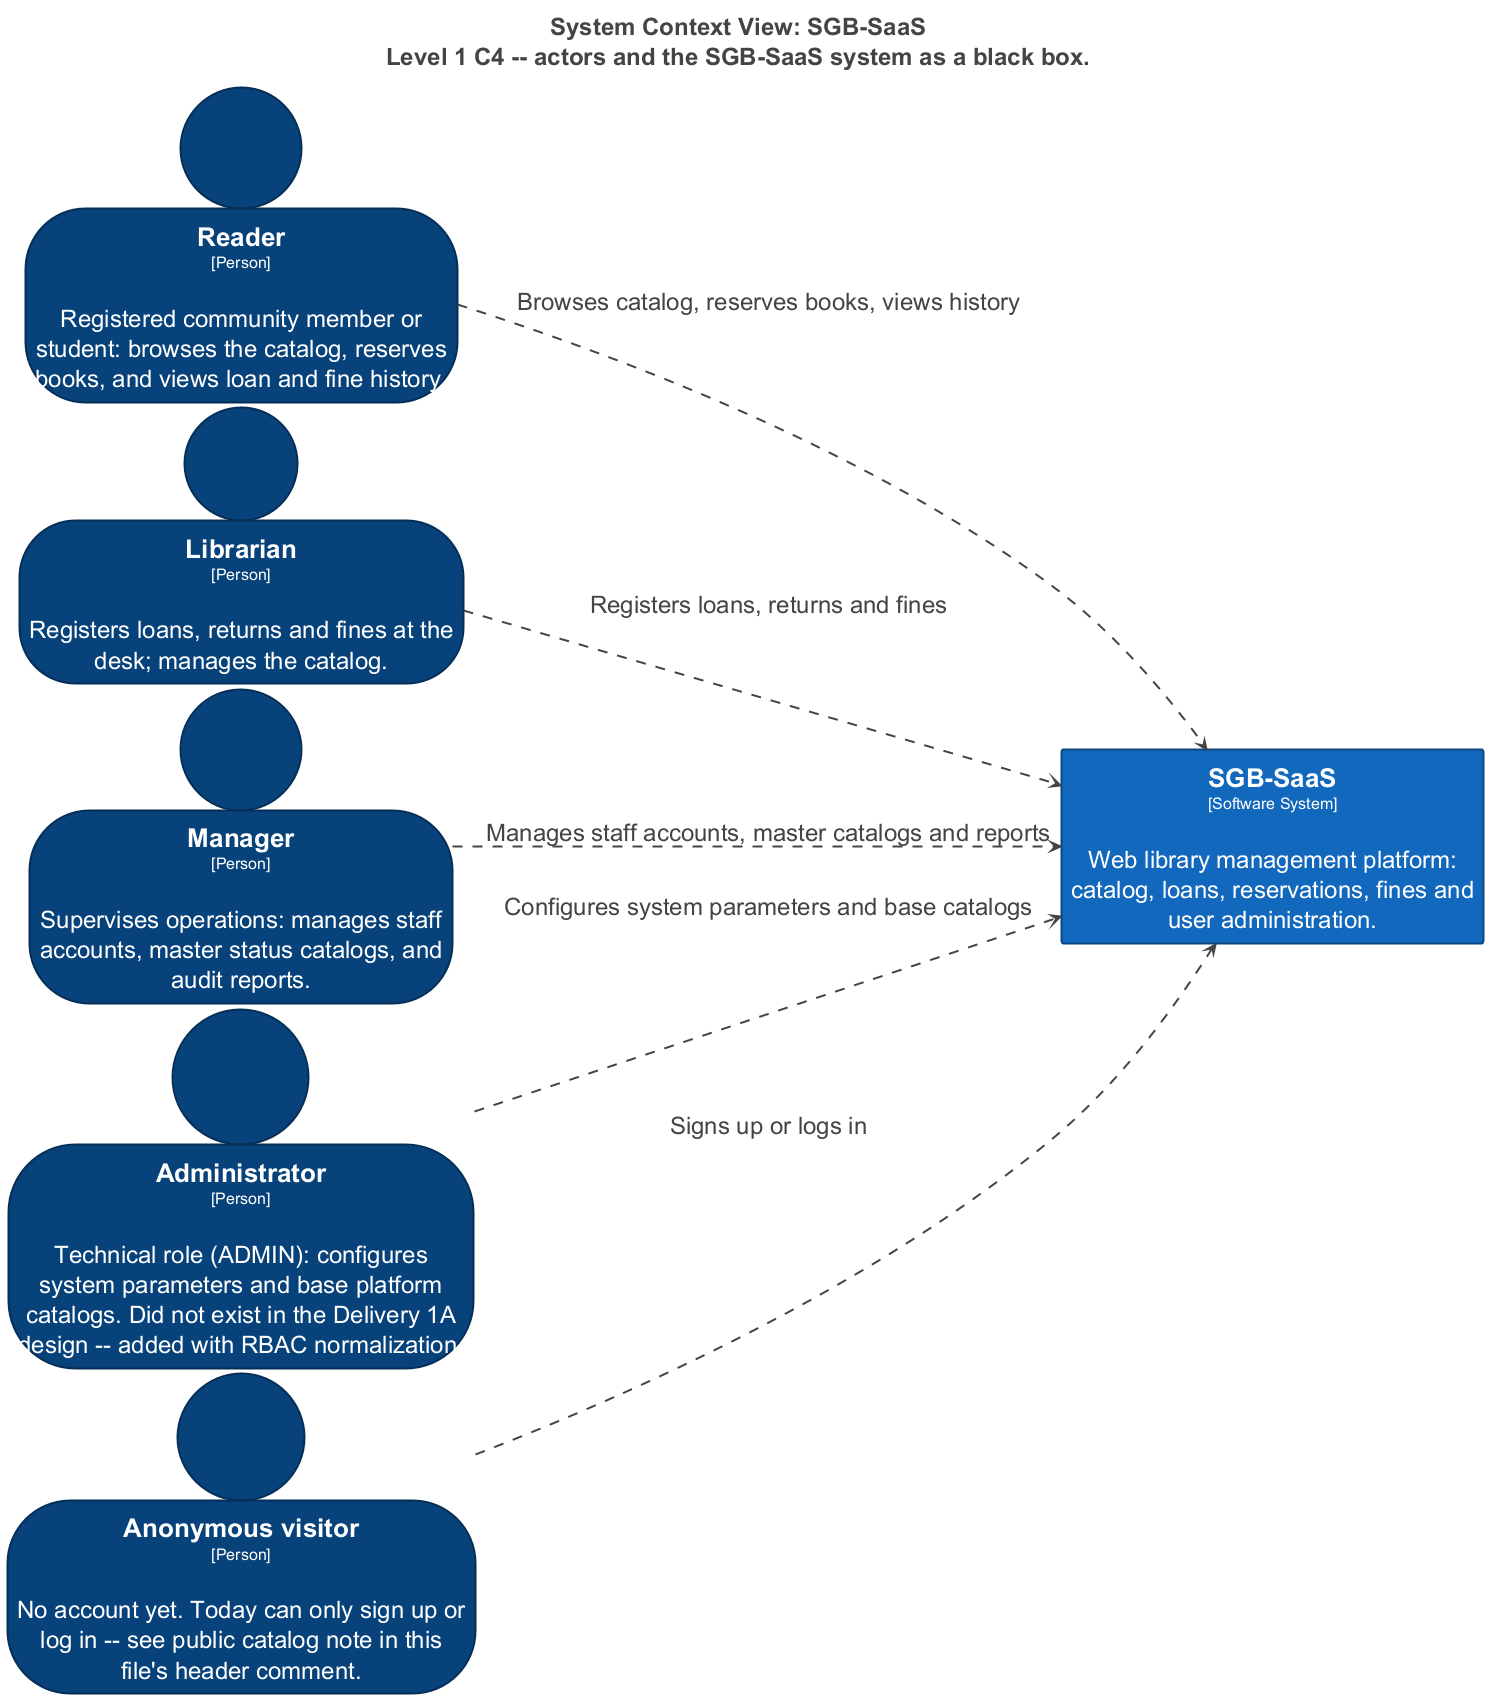
\includegraphics[width=0.85\textwidth]{arquitectura/c4-nivel1-contexto.png}
\caption{Modelo C4, Nivel~1 (Contexto): los cinco actores del sistema
y sus interacciones con SGB-SaaS como caja negra. Exportado
automáticamente desde \texttt{workspace.dsl}.}
\label{fig:c4-nivel1-contexto}
\end{figure}

\begin{figure}[h]
\centering
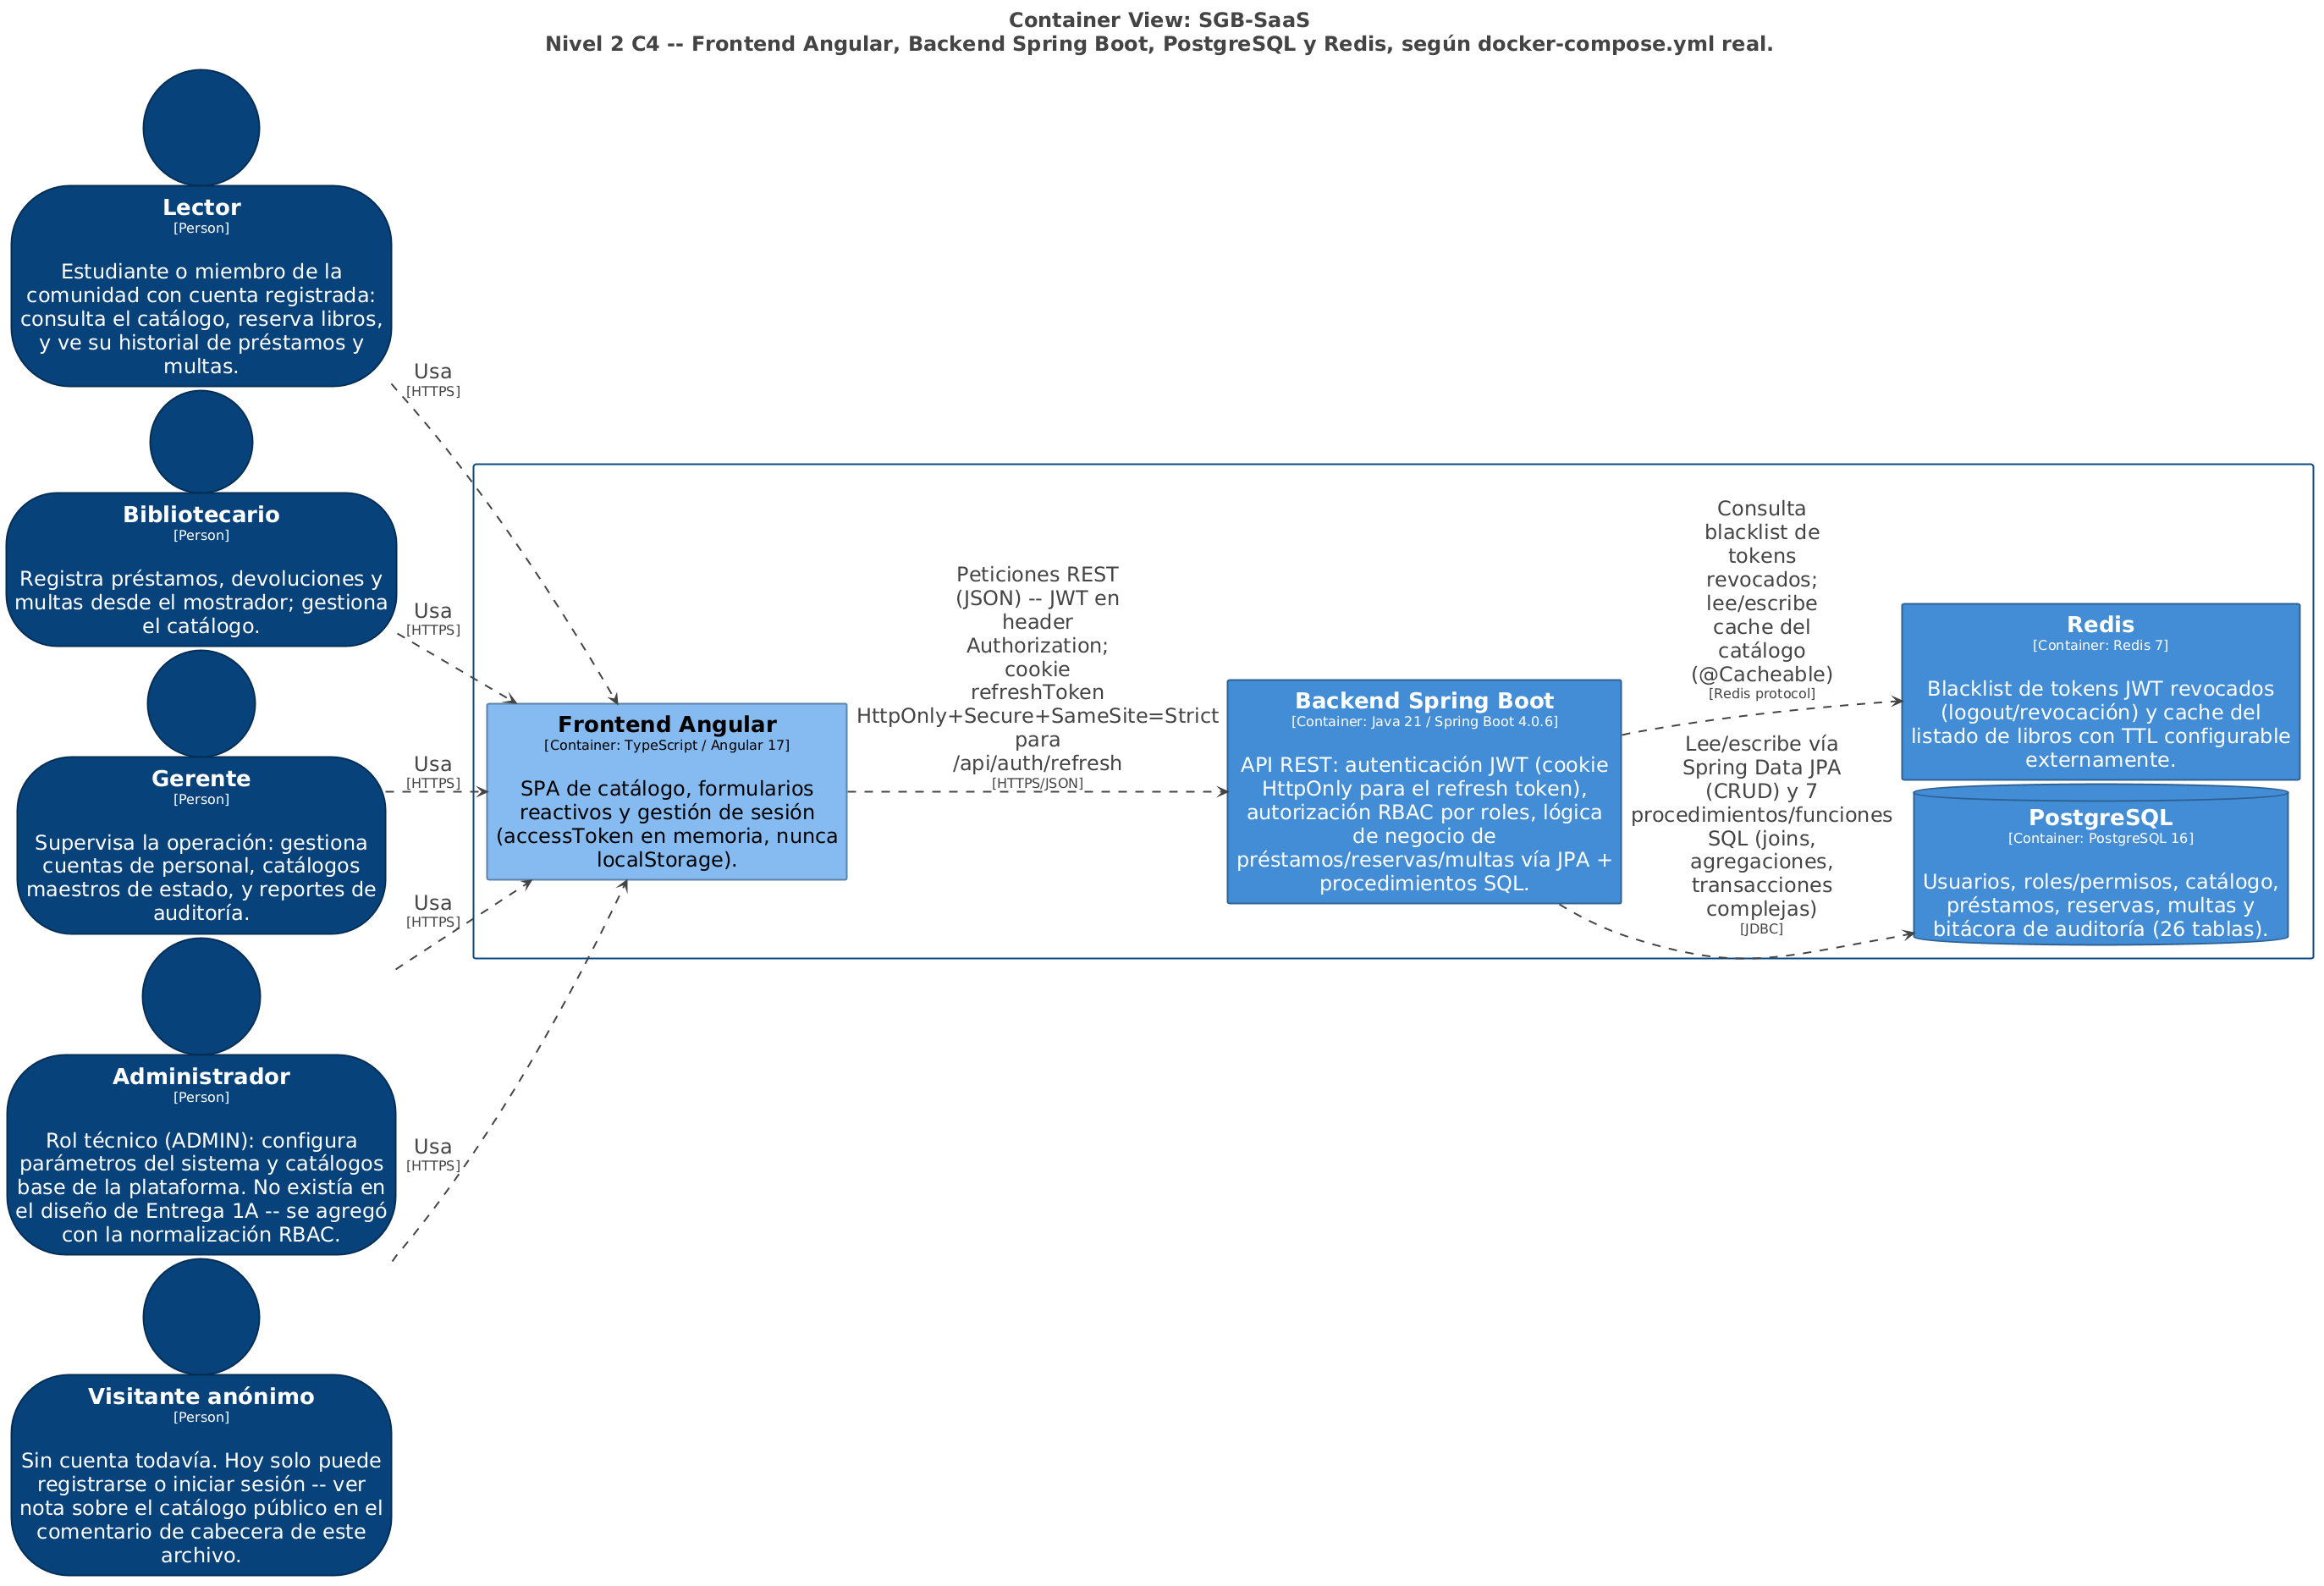
\includegraphics[width=0.95\textwidth]{arquitectura/c4-nivel2-contenedores.png}
\caption{Modelo C4, Nivel~2 (Contenedores): Frontend Angular, Backend
Spring Boot, PostgreSQL y Redis, alineados 1:1 con
\texttt{docker-compose.yml}. Exportado automáticamente desde
\texttt{workspace.dsl}.}
\label{fig:c4-nivel2-contenedores}
\end{figure}

\section{Nivel 1 -- Contexto del sistema}

Cinco actores interactúan con SGB-SaaS como caja negra: \textbf{Lector}
(consulta el catálogo, reserva libros, ve su historial de préstamos y
multas), \textbf{Bibliotecario} (registra préstamos, devoluciones y
multas desde el mostrador; gestiona el catálogo),
\textbf{Gerente} (supervisa la operación: cuentas de personal, catálogos
maestros de estado y reportes de auditoría), \textbf{Administrador}
(configura parámetros del sistema y catálogos base de la plataforma --
rol que no existía en el diseño original de Entrega~1A, incorporado al
normalizar el modelo RBAC) y \textbf{Visitante anónimo} (sin cuenta
todavía; hoy solo puede registrarse o iniciar sesión).

El propio \texttt{workspace.dsl} documenta, en su comentario de
cabecera, una discrepancia real entre el diseño original de Entrega~1A y
la implementación actual que vale la pena señalar aquí: Gemini~3.5~Flash~Lite
API y Google Books API aparecían como sistemas externos en el diseño
original y se \textbf{retiraron} del diagrama actual porque no existe
ninguna integración con Google Books en el código real (Gemini sí se
integró, pero como parte interna del contenedor Backend, no como un
"sistema externo" del Nivel~1 -- ver \autoref{sec:c4-nivel3} más
abajo). Tampoco se
diseñó nunca un endpoint de catálogo público accesible sin
autenticación: \texttt{LibroController} exige rol \texttt{LECTOR} (o
superior) incluso para listar libros, así que el alcance real del
\emph{Visitante anónimo} se limita a registro e inicio de sesión.

\section{Nivel 2 -- Contenedores}

Cuatro contenedores, alineados 1:1 con \texttt{docker-compose.yml}:

\begin{itemize}[leftmargin=1.2cm]
  \item \textbf{Frontend Angular} (TypeScript/Angular~21) -- SPA de
    catálogo, formularios reactivos y gestión de sesión con el
    \texttt{accessToken} en memoria, nunca en \texttt{localStorage}.
  \item \textbf{Backend Spring Boot} (Java~21/Spring~Boot~4.0.6) -- API
    REST con autenticación JWT (cookie \texttt{HttpOnly} para el
    \texttt{refreshToken}), autorización RBAC por roles, y lógica de
    negocio de préstamos/reservas/multas vía JPA y procedimientos SQL.
  \item \textbf{PostgreSQL~16} -- usuarios, roles/permisos, catálogo,
    préstamos, reservas, multas y bitácora de auditoría (26 tablas).
  \item \textbf{Redis~7} -- blacklist de tokens JWT revocados (logout /
    revocación) y caché del listado de libros con TTL configurable
    externamente.
  \end{itemize}

El diagrama entidad-relación real del esquema PostgreSQL
(\autoref{fig:der-real}) se generó automáticamente aplicando, en orden
numérico, las 35 migraciones Flyway de \texttt{database/migrations/}
(\texttt{V1} a \texttt{V36}, con el hueco ya documentado en
\texttt{V29}) sobre una instancia PostgreSQL~16 real y limpia, y
extrayendo el esquema resultante con \texttt{eralchemy2}. El resultado
tiene 44 tablas -- más que las 26 citadas en la enumeración de arriba,
cifra que no se corrige aquí por quedar fuera del alcance de esta
tarea puntual; ver nota en el reporte de esta sesión.

\begin{figure}[h]
\centering
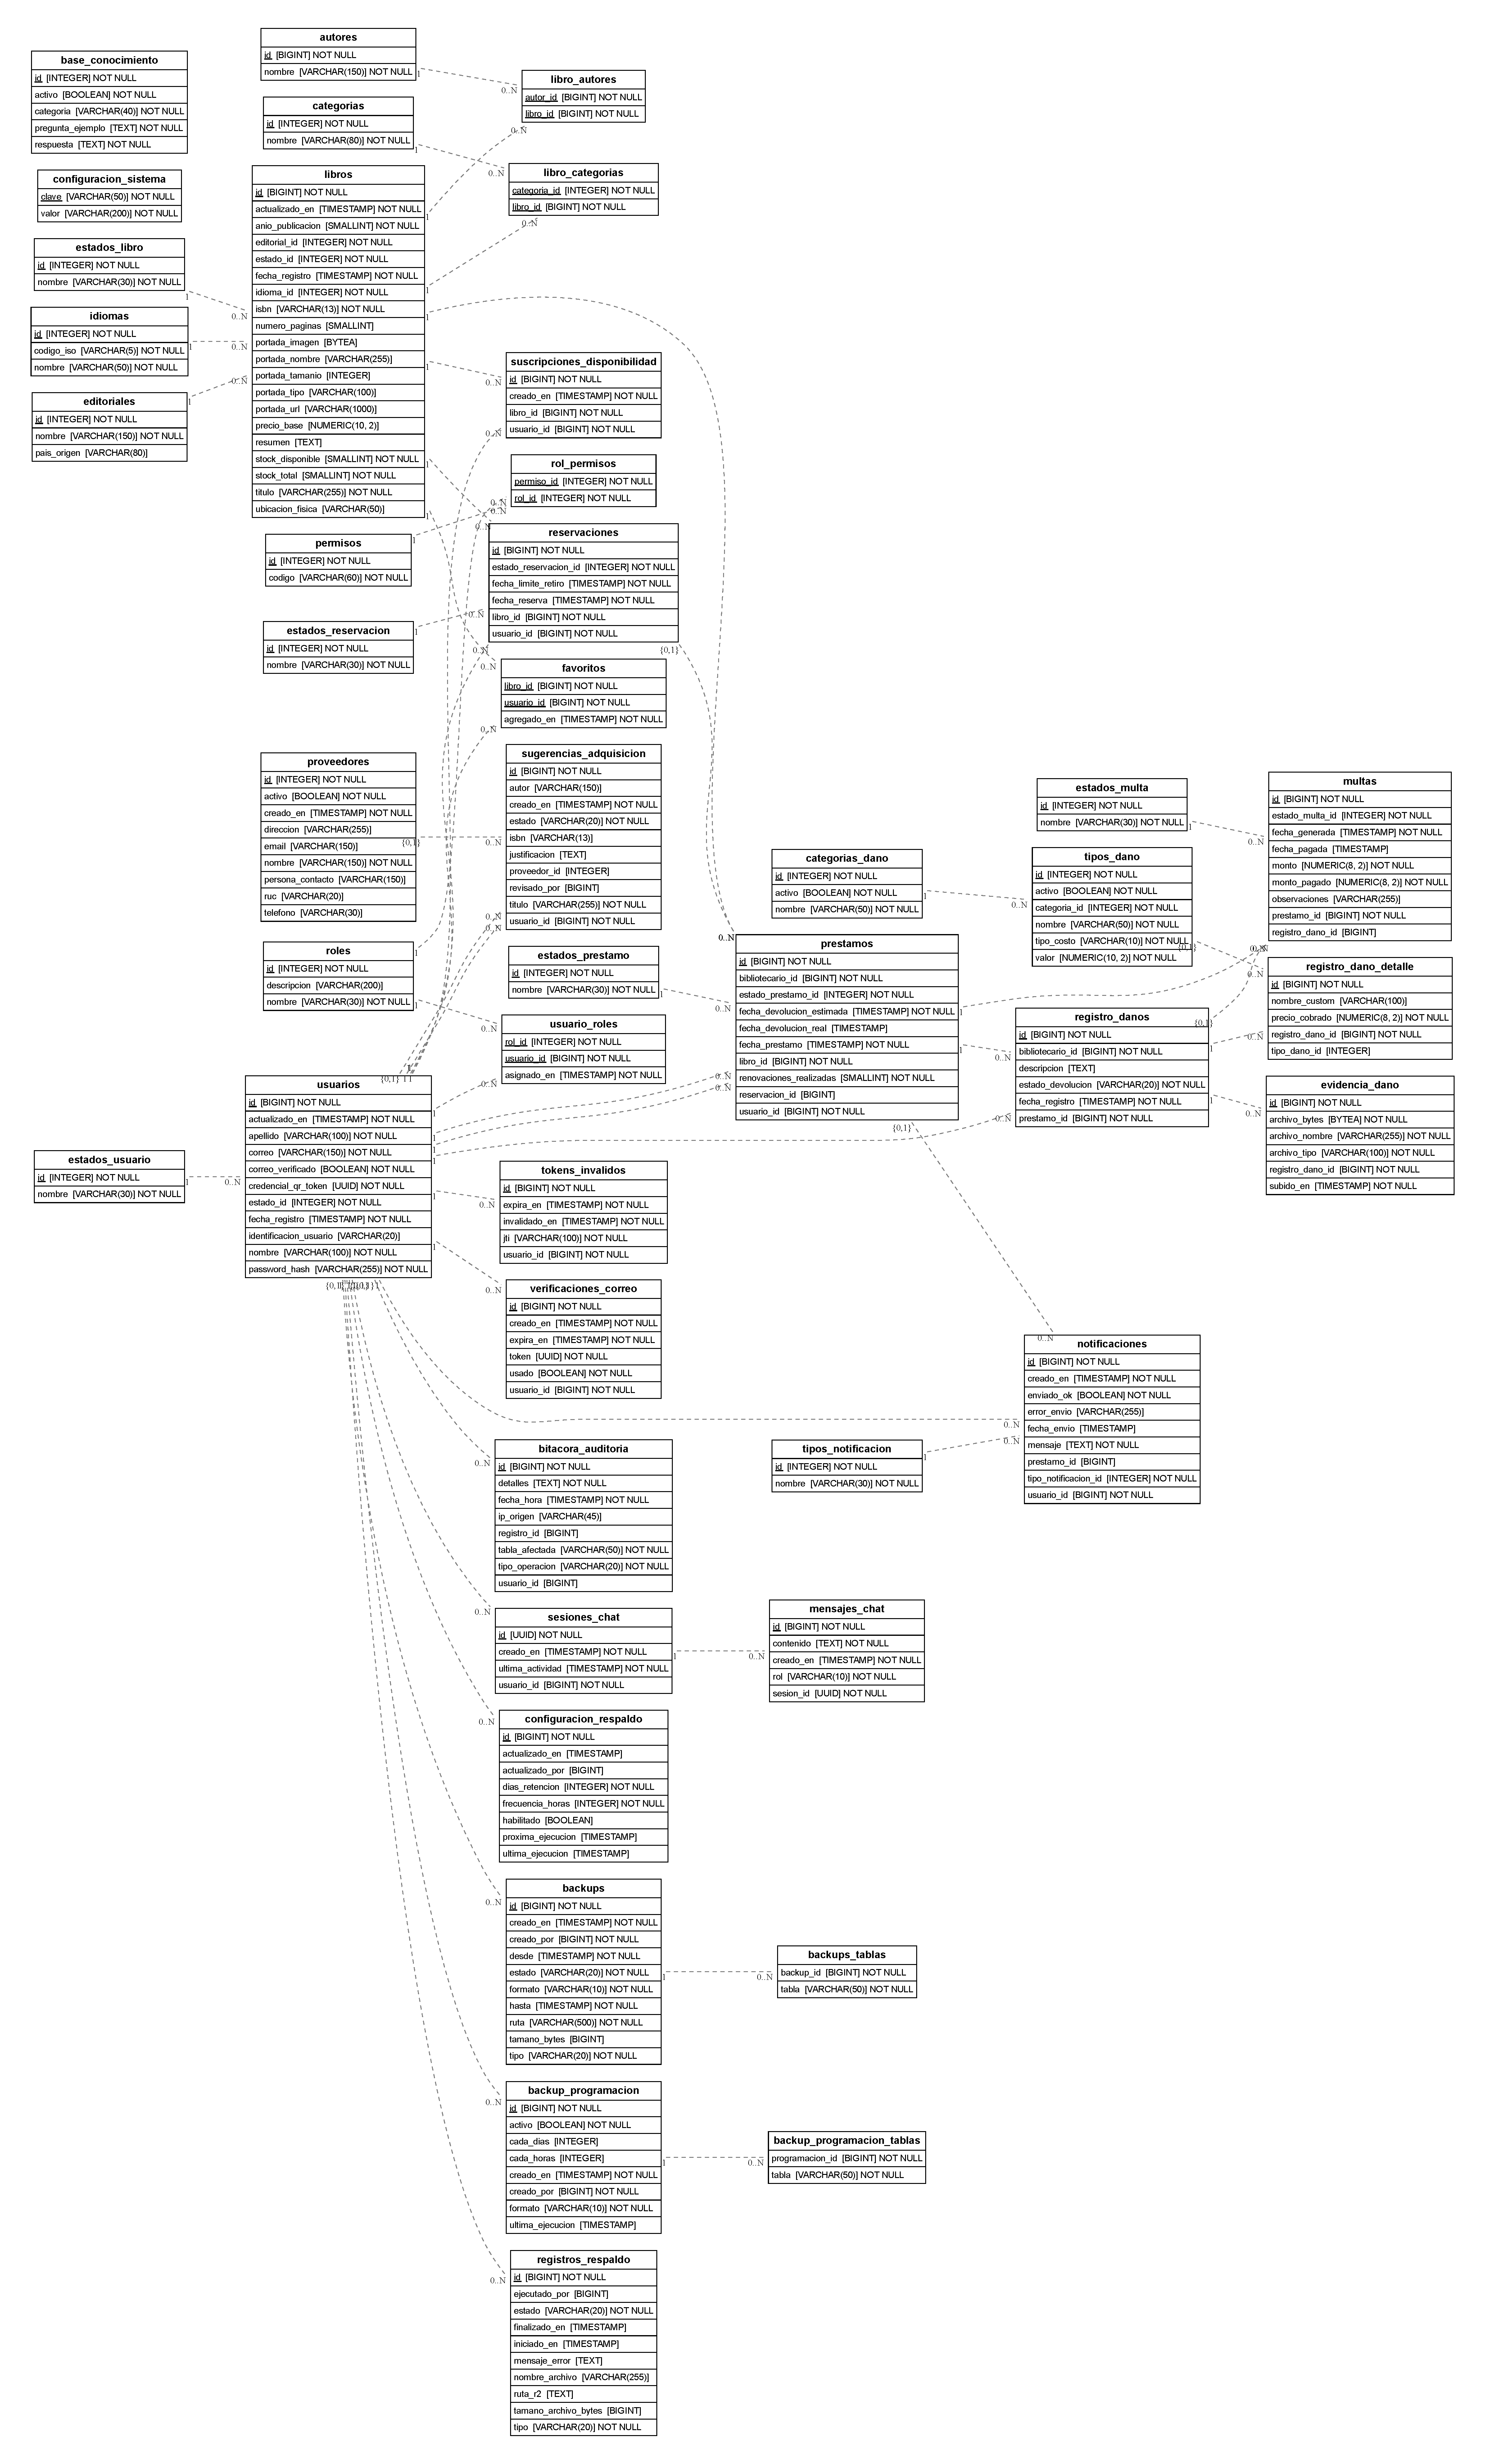
\includegraphics[width=0.95\textwidth]{diagramas/der-real.pdf}
\caption{Diagrama entidad-relación real, generado automáticamente con
\texttt{eralchemy2} a partir del esquema PostgreSQL reconstruido desde
las 35 migraciones Flyway de \texttt{database/migrations/}. Reemplaza
a \texttt{docs/diagramas/Diagrama\_ER.png}, que correspondía por error
a un dominio clínico ajeno a este proyecto (ver OBS-21 en
\texttt{docs/observaciones/OBSERVACIONES.md}).}
\label{fig:der-real}
\end{figure}

Respecto al diseño original de Entrega~1A, el contenedor Redis y el
actor Administrador son incorporaciones directas de la normalización
RBAC y del mecanismo de revocación de tokens vía \emph{blacklist}, ambos
ausentes del diagrama de contenedores original.

\section{Nivel 3 -- Componentes}
\label{sec:c4-nivel3}

El Nivel~3 se completó una vez cerradas las 8 ramas del módulo de
Préstamos/Reservas/Multas (evitando así reconstruir el diagrama dos
veces mientras ese módulo seguía en desarrollo activo). Se construyó a
partir del inventario real de \emph{controllers}/\emph{services}/clases
de seguridad del backend -- no del diseño aspiracional --, agrupado por
dominio en 21 componentes para mantener el diagrama legible en vez de
tener una entrada por cada una de las cerca de 30 clases reales:

\begin{itemize}[leftmargin=1.2cm]
  \item \textbf{Capa API} (7 componentes): Auth~API, Catálogo~API,
    Préstamos~API, Notificaciones~API, CredencialQR~API, Chatbot~API,
    Admin~API -- un componente por dominio funcional, no por clase
    \texttt{@RestController} individual.
  \item \textbf{Capa de servicio} (8 componentes): Auth~Service,
    Catálogo~Service, Préstamos~Service, Reportes~Service,
    Notificaciones~Service, CredencialQR~Service, Chatbot~Service, Admin
    Service.
  \item \textbf{Seguridad} (5 componentes): \texttt{JwtService},
    \texttt{JwtAuthFilter}, \texttt{UserDetailsServiceImpl},
    \texttt{LoginRateLimiter} (OWASP A07, límite de intentos de login por
    correo+IP) y \texttt{ChatbotRateLimiter} (límite de mensajes al
    asistente por usuario).
  \item \textbf{Integración externa} (1 componente): \texttt{GeminiClient}
    -- cliente HTTP hacia la API de Gemini~3.5~Flash~Lite, con reintento
    simple ante 429/timeout/5xx y sin exponer la URL con la API key en
    logs (ver ADR-016, \autoref{sec:adrs}).
\end{itemize}

Las relaciones entre componentes se verificaron contra el código real
(no se infirieron): cada flecha API~$\to$~Service, Service~$\to$~Postgres/
Redis, y las dependencias cruzadas de \texttt{ChatbotService} hacia
\texttt{CatálogoService} y \texttt{PréstamosService} para el
\emph{grounding} real de sus respuestas (consulta disponibilidad de
libros y reservas del propio usuario antes de responder, para no
inventar disponibilidad) corresponden a llamadas reales entre las
clases Java correspondientes.

\subsection*{Validación sintáctica y exportación visual}
\label{sec:c4-exportacion}

El archivo se validó sintácticamente con el motor activamente mantenido
\texttt{structurizr/structurizr} (subcomando \texttt{validate}), no con
\texttt{structurizr/cli} -- que en este momento del ecosistema
Structurizr es una imagen retirada que solo imprime un aviso de
desuso y termina con código de salida~0 para cualquier entrada, válida o
no (confirmado también al intentar el \texttt{export} con esa imagen:
código de salida~0 sin generar ningún archivo), por lo que una
validación o exportación con esa imagen no habría sido real. Los tres
niveles se exportaron con el mismo flujo activamente mantenido:
\texttt{structurizr/structurizr export -workspace workspace.dsl
-format plantuml}, seguido de renderizado con PlantUML
(\texttt{plantuml/plantuml} vía Docker). El diagrama de Nivel~3
resultó en \texttt{docs/arquitectura/c4-nivel3-componentes.svg}
(generado en una sesión previa; se confirmó en esta sesión que sigue
coincidiendo con el \texttt{workspace.dsl} vigente -- mismos 21
componentes, mismas relaciones -- por lo que no fue necesario
regenerarlo), versionado junto al DSL fuente y reproducido en la
\autoref{fig:c4-componentes}. Los diagramas de Nivel~1 y Nivel~2 se
exportaron en esta sesión de la misma forma, resultando en
\texttt{docs/arquitectura/c4-nivel1-contexto.png} y
\texttt{c4-nivel2-contenedores.png}, reproducidos en la
\autoref{fig:c4-nivel1-contexto} y la \autoref{fig:c4-nivel2-contenedores}.

\begin{figure}[h]
\centering
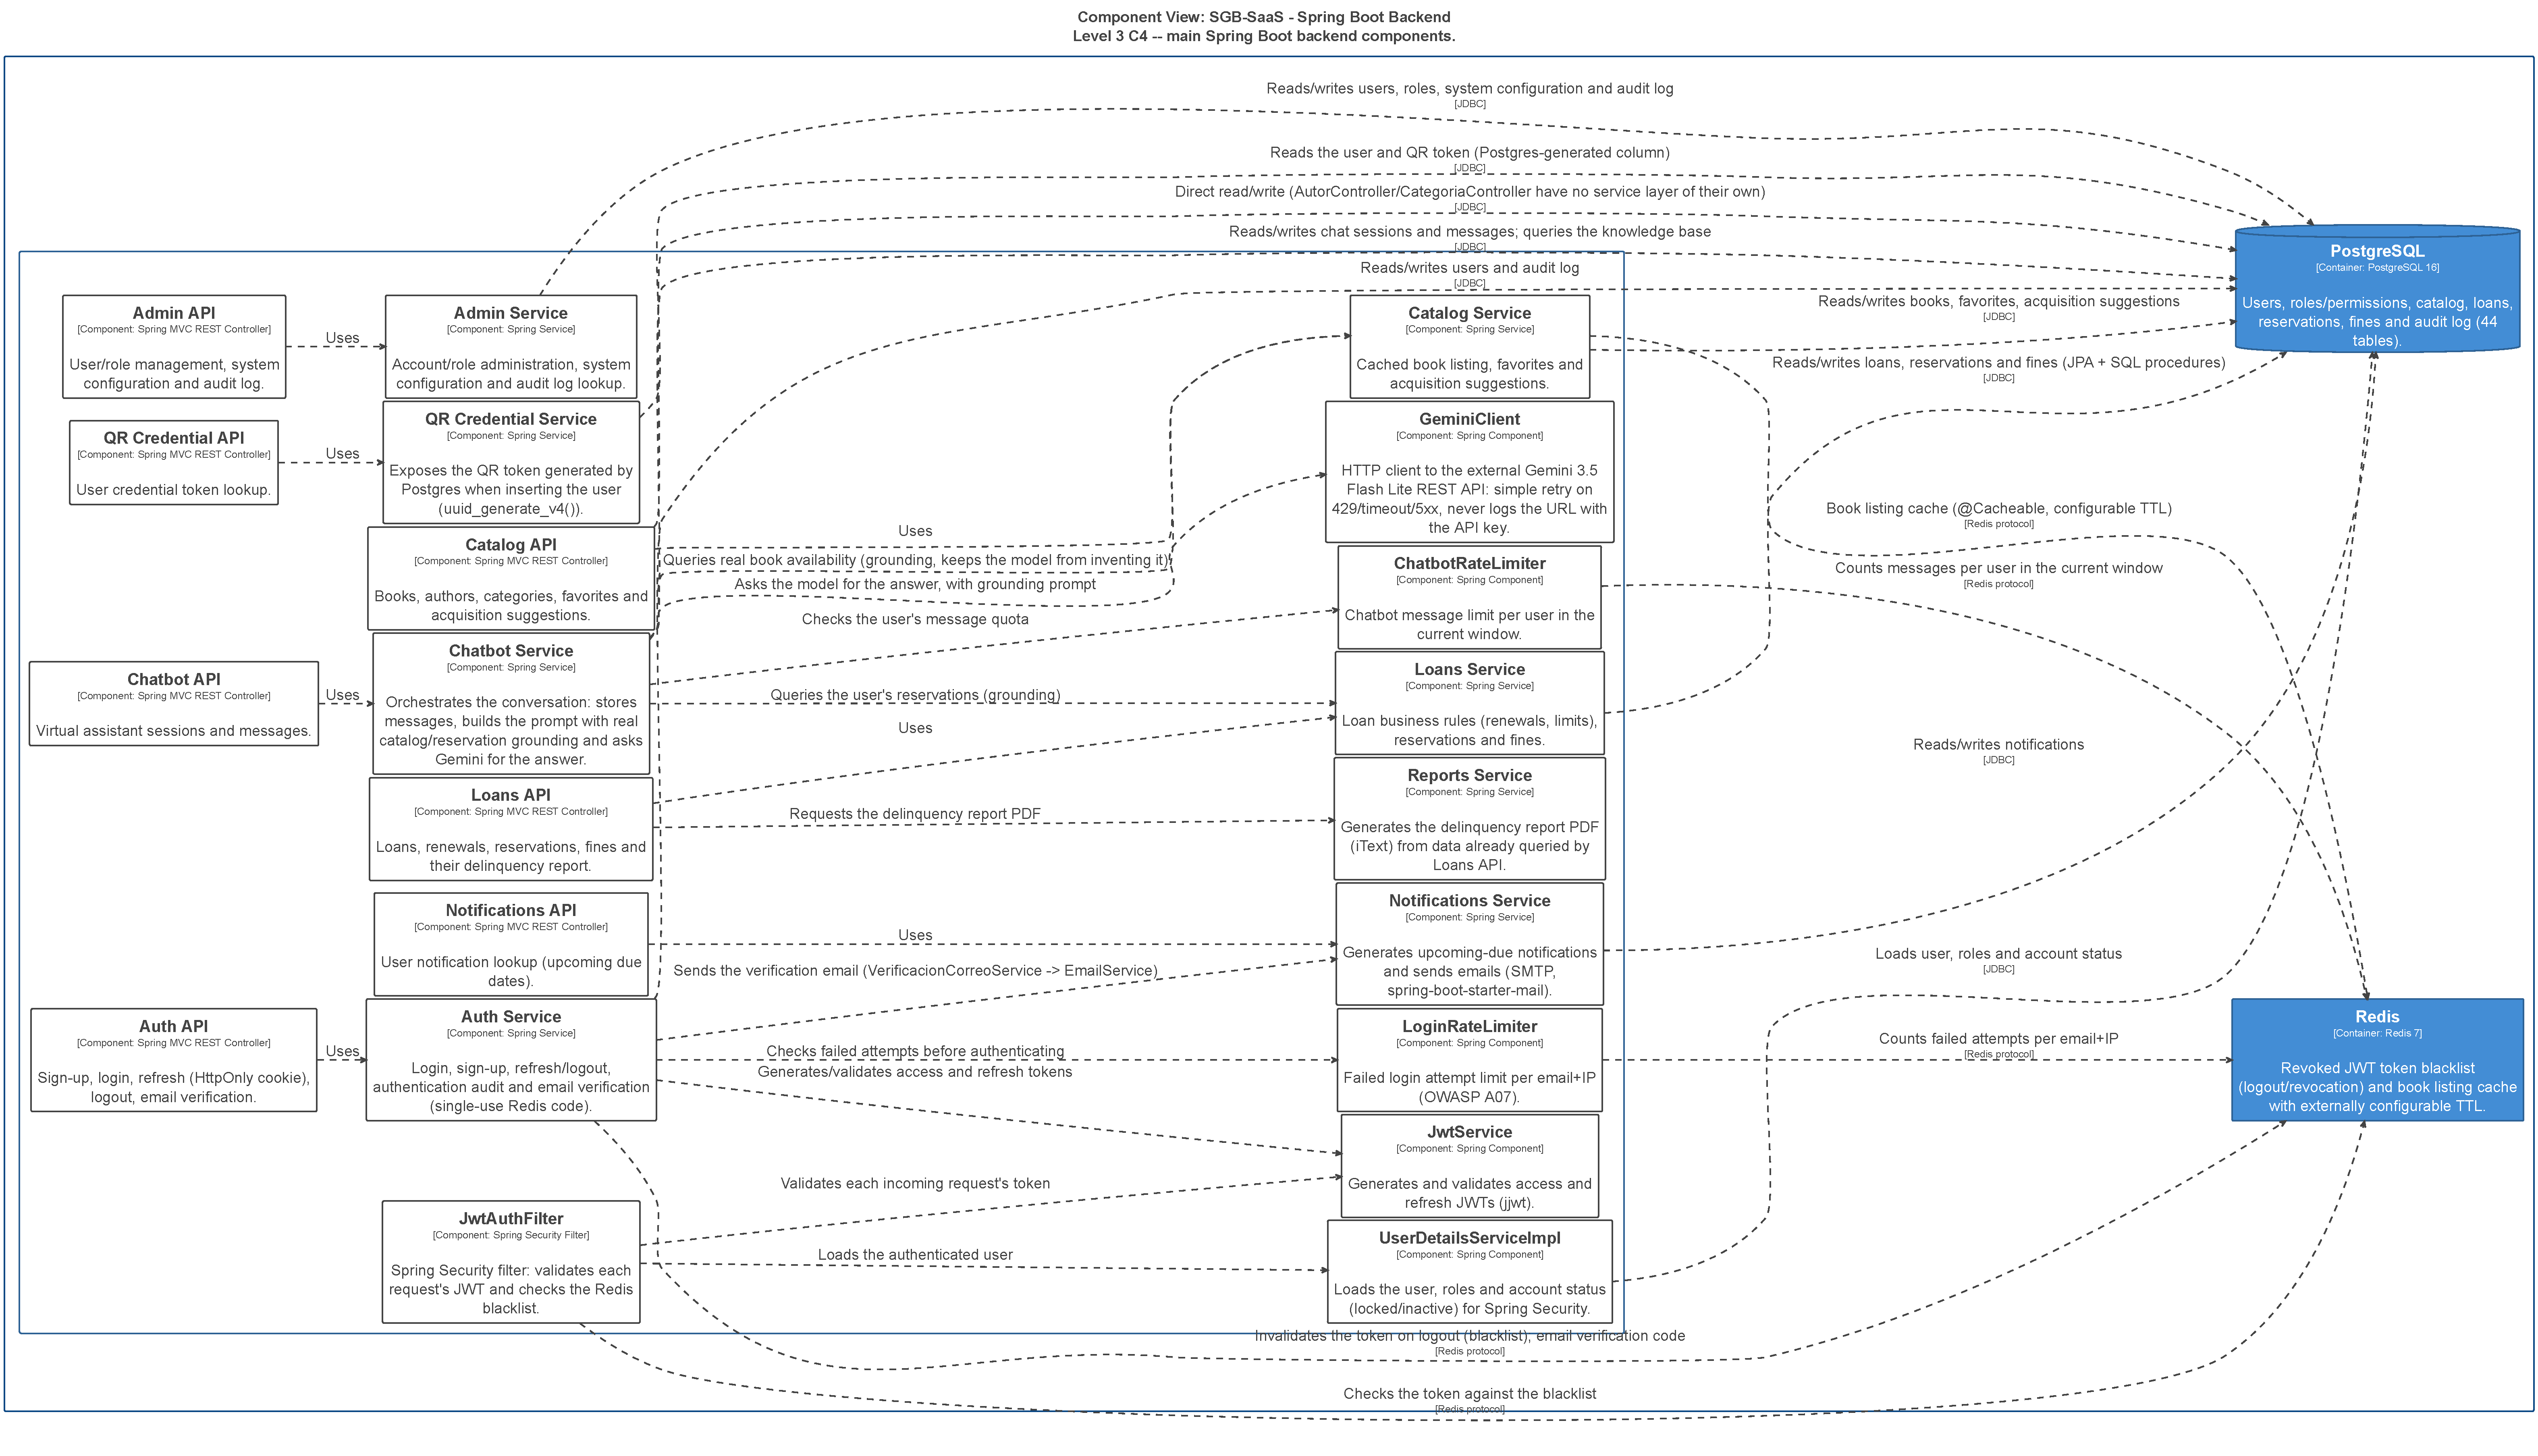
\includegraphics[width=\textwidth]{arquitectura/c4-nivel3-componentes.pdf}
\caption{Modelo C4, Nivel~3 (Componentes) del backend Spring Boot -- 21
componentes agrupados por dominio (capa API, capa de servicio,
seguridad e integración externa), con sus relaciones verificadas contra
el código real. Conversión a PDF del SVG fuente versionado en
\texttt{docs/arquitectura/c4-nivel3-componentes.svg} (pdflatex no
soporta SVG directamente).}
\label{fig:c4-componentes}
\end{figure}

\section{Decisiones arquitectónicas documentadas (ADR)}
\label{sec:adrs}

El repositorio contiene \textbf{13 Architecture Decision Records}
(\texttt{docs/adr/}), agrupados a continuación según los 6 temas
obligatorios del Bloque~D de la guía (mapeo completo en
\texttt{docs/adr/README.md}). Hasta el 26 de agosto de 2026, dos de esos
temas estaban cubiertos por un ADR cuya numeración interna del
repositorio no coincidía con la numeración sugerida por la guía
(\texttt{ADR-006}/\texttt{ADR-007} sugeridos por la guía para acceso a
datos y despliegue correspondían a \texttt{ADR-013} y \texttt{ADR-012}
en este repositorio), por continuidad con la numeración ya evaluada en
la Tercera Entrega. Se decidió renumerar de todas formas para que la
numeración coincida literalmente con la guía en vez de dejarlo como una
diferencia solo explicada en prosa -- ver la nota histórica en
\texttt{docs/adr/README.md} con el detalle del intercambio y las
referencias cruzadas actualizadas en el mismo cambio.

\begin{center}
\small
\begin{tabularx}{\linewidth}{|c|X|l|}
\hline
\rowcolor{verdeuteq}
\color{white}\textbf{\#} & \color{white}\textbf{Tema obligatorio (Bloque D)} & \color{white}\textbf{ADR(s)} \\
\hline
1 & Elección de la pila tecnológica principal & \texttt{ADR-001} \\
\hline
2 & Esquema de autenticación & \texttt{ADR-010} + \texttt{ADR-003} + \texttt{ADR-012} \\
\hline
3 & Gestor de base de datos & \texttt{ADR-011} \\
\hline
4 & Estrategia de caché & \texttt{ADR-008} \\
\hline
5 & Estrategia de despliegue & \texttt{ADR-007} \\
\hline
6 & Estrategia de acceso a datos (CRUD-ORM vs.\ SP) & \texttt{ADR-006} \\
\hline
\end{tabularx}
\end{center}

Los 7 ADR restantes no mapean a ninguno de los 6 temas obligatorios,
pero documentan decisiones reales tomadas durante el desarrollo:
\texttt{ADR-013} (versionado de esquema reproducible, Flyway + snapshot),
\texttt{ADR-009} (licencia MIT), \texttt{ADR-014} (separación de
responsabilidades entre \texttt{ADMIN} y \texttt{GERENTE}: el primero
administra permisos/configuración de plataforma, el segundo la operación
diaria -- ninguno de los dos queda excluido de \emph{ver} el padrón de
usuarios, pero solo \texttt{ADMIN} puede \emph{modificarlo}),
\texttt{ADR-015} (TLS termina en el proxy, no en el backend Spring
Boot: el backend queda preparado vía
\texttt{server.forward-headers-strategy: framework} para reconocer
\texttt{X-Forwarded-Proto} y activar HSTS el día que el proxy real
active TLS, sin cambios de código adicionales), y \texttt{ADR-016}
(qué datos exactos viajan a la API externa de Gemini en el chatbot --
texto del mensaje, historial de la sesión y un prompt de
\emph{grounding} con datos ya públicos del catálogo -- y por qué eso no
constituye una exposición indebida de información: nunca viajan
credenciales, tokens, contraseñas ni identificación personal).

\section{Atributos de calidad (ISO/IEC 25010)}

Aplicando el modelo de calidad descrito en la \autoref{sec:mt-25010},
\texttt{docs/arquitectura/ISO25010.md} prioriza las 8 características de
calidad de producto de la norma para el contexto específico de este
proyecto (biblioteca universitaria de bajo volumen, no un sistema de
alta concurrencia), citando evidencia real donde existe en vez de
estimarla. Se reproduce a continuación tal cual el documento fuente
(única fuente de verdad de esta tabla; este capítulo no la duplica de
memoria):

\begin{center}
\small
\begin{longtable}{|l|c|p{8.7cm}|}
\hline
\rowcolor{verdeuteq}
\color{white}\textbf{Característica} & \color{white}\textbf{Prioridad} & \color{white}\textbf{Estrategia / decisión que la atiende} \\
\hline
\endhead
Adecuación funcional & Alta & Procedimientos almacenados transaccionales para operaciones con lógica cruzada multi-tabla (\texttt{sp\_registrar\_devolucion}, \texttt{sp\_pagar\_multa}, \texttt{sp\_anular\_multa}), constraints de integridad referencial (FKs, CHECKs) en \texttt{db/schema.sql}. \\
\hline
Eficiencia de desempeño & Media & Caché Redis del listado de libros con TTL externo (ADR-008). Evidencia vigente: prueba de carga formal (50~VUs, 5 corridas de k6 con Wilcoxon + Cliff's delta) -- p95 agregado \textbf{19{,}49\,ms} en \texttt{cache\_caliente} (umbral $<$200\,ms) y \textbf{7{,}50\,ms} en \texttt{cache\_frio} (umbral $<$500\,ms), 0\,\% de errores 5xx en 20\,003 peticiones (\texttt{docs/mediciones/perf/REPORT.md}). El propio informe declara una limitación metodológica real (ver \autoref{cap:amenazas-validez}): \texttt{cache\_frio} mide sobre todo consultas con página vacía, no el costo real de traer una página llena sin caché. Una medición manual preliminar del 21 de julio había reportado cifras de otro orden de magnitud ($\sim$170\,ms/$\sim$30\,ms) por tratarse de una sola petición aislada sin carga concurrente; queda solo como antecedente histórico, no como evidencia vigente. \\
\hline
Compatibilidad & Media & API REST documentada con OpenAPI/Swagger vía springdoc-openapi (ADR-001), JSON como formato estándar -- sin integración real hoy con sistemas académicos institucionales ni con Google Books API. \\
\hline
Usabilidad & Alta & \texttt{sp\_registrar\_devolucion} valida el estado del préstamo antes de actuar (rechaza con \texttt{LB409} si ya estaba devuelto, evitando duplicidad); frontend Angular con formularios reactivos y validación antes de enviar. \\
\hline
Fiabilidad & Alta & Parcialmente atendida: ADR-003 documenta explícitamente que, si Redis cae, \texttt{JwtAuthFilter} queda sin forma de verificar revocaciones -- la decisión \emph{fail-open} vs.\ \emph{fail-closed} sigue anotada como pendiente para producción, no resuelta. Los \emph{healthchecks} de \texttt{docker-compose.yml} sí garantizan un orden de arranque correcto. \\
\hline
Seguridad & Alta & Cookie \texttt{HttpOnly+Secure+SameSite=None} para el \texttt{refreshToken} (ADR-012), BCrypt costo 12, blacklist de tokens revocados (ADR-003), respuestas de error RFC~7807 sin fuga de detalles internos. \textbf{Nota de este informe}\footnote{\texttt{SameSite=None} era necesario para que el navegador enviara la cookie entre los orígenes cross-origin de Render (frontend y backend en subdominios distintos), pero reintroduce la exposición a CSRF que \texttt{SameSite=Strict} bloqueaba por sí solo. El código actual tiene \texttt{.csrf(csrf -> csrf.disable())} activo (\texttt{SecurityConfig.java}, línea 55) y no implementa ningún token CSRF; el único control vigente es la lista blanca de CORS, que impide leer la respuesta cross-origin pero no impide el envío de la petición con la cookie adjunta. El ADR-012 documenta esto explícitamente como riesgo aceptado, no mitigado, con la corrección (token CSRF / \emph{double-submit cookie}) registrada como trabajo futuro (\autoref{sec:tf-csrf}).}: el diseño actual acepta explícitamente el riesgo de CSRF residual sobre \texttt{/api/auth/refresh} que introduce \texttt{SameSite=None}, según ADR-012 -- ver aclaración al pie. \\
\hline
Mantenibilidad & Alta & Los ADR de \texttt{docs/adr/} documentan decisiones no obvias con sus alternativas consideradas; \texttt{docs/basedatos/CATALOGO-SP.md} documenta el criterio de separación CRUD-ORM vs.\ procedimientos. \textbf{Nota de este informe}\footnote{El texto original de \texttt{ISO25010.md} en esta fila cita ``6 ADRs existentes'', cifra que quedó desactualizada tras incorporar los 8 módulos construidos después de la Tercera Entrega -- el repositorio contiene 13 ADRs a la fecha de este capítulo (\autoref{sec:adrs}). Se transcribe el texto original de la fuente junto con esta aclaración en vez de editarlo silenciosamente, ya que corregir \texttt{ISO25010.md} está fuera del alcance de esta tarea.}: la cifra real de ADRs es 13, no 6 -- ver aclaración al pie. \\
\hline
Portabilidad & Alta & Docker Compose con imágenes base pinadas por digest sha256, \texttt{db/init/01-consolidado.sql} generado de forma reproducible, arranque de un solo comando vía \texttt{make up}. \\
\hline
\end{longtable}
\end{center}

\section{Matriz de trazabilidad -- resumen por tipo de acceso a datos}
\label{sec:matriz-resumen}

La matriz completa de los 46 requisitos vive en
\texttt{docs/trazabilidad/matriz.csv} y se valida automáticamente en
cada ejecución de CI vía \texttt{scripts/validate-traceability.sh}. Este
capítulo no reproduce las 46 filas (el detalle completo por requisito
vive en \autoref{cap:ingenieria-requisitos} y en la propia matriz);
resume aquí la columna \texttt{tipo\_acceso}, relevante para esta
sección por ser la evidencia directa de que la estrategia híbrida
CRUD-ORM/SP declarada en ADR-006 se aplica de verdad y no solo en
teoría.

\textbf{Nota de corrección respecto a una versión anterior de este
capítulo.} \texttt{matriz.csv} tenía 4 filas
(\texttt{REQ-F-018}, \texttt{REQ-F-019}, \texttt{REQ-F-020},
\texttt{REQ-F-028}) con una coma sin escapar dentro de un campo, que
rompía el parseo CSV estándar -- defecto ya corregido en el commit
\texttt{ecfaf52}. Una versión anterior de esta tabla, calculada antes de
esa corrección, solo había detectado 2 de las 4 filas afectadas
(\texttt{REQ-F-019}, \texttt{REQ-F-020}) y las marcaba como ``sin
clasificar''; además atribuía el problema de \texttt{REQ-F-019} a la
columna \texttt{tipo\_acceso}, cuando en realidad ese campo sí tenía un
valor de \texttt{tipo\_acceso} válido (\texttt{"CRUD-ORM + generacion de
imagen (ZXing)"}) -- el campo roto en esa fila específica era
\texttt{modulo\_codigo}, no \texttt{tipo\_acceso}. Con las 43 filas
parseando limpio, la tabla de abajo reclasifica las 4 filas
correctamente en vez de dejarlas fuera:

\begin{center}
\begin{tabularx}{\linewidth}{|X|c|c|}
\hline
\rowcolor{verdeuteq}
\color{white}\textbf{Tipo de acceso a datos} & \color{white}\textbf{Requisitos} & \color{white}\textbf{\%} \\
\hline
CRUD-ORM (exclusivo, incl.\ combinado con Redis/SMTP/caché/API externa) & 21 & 48{,}8\,\% \\
\hline
Híbrido SP + CRUD-ORM (requisitos transversales) & 2 & 4{,}7\,\% \\
\hline
Procedimiento/función SQL (SP, exclusivo, incl.\ combinado con generación de PDF) & 8 & 18{,}6\,\% \\
\hline
No aplica (decisión de arquitectura, configuración, control de acceso o UI sin acceso directo a BD) & 11 & 25{,}6\,\% \\
\hline
Redis + SMTP (sin tabla Postgres nueva; no aplica CRUD-ORM ni SP)\footnote{\texttt{REQ-F-020}: \texttt{tipo\_acceso} = ``Redis (código OTP con TTL, sin tabla nueva) + SMTP (EmailService)''. Categoría propia, no un defecto de la matriz -- el código de verificación vive en Redis con TTL, sin persistirse en una tabla Postgres nueva, y el envío usa SMTP directo; no encaja limpiamente en CRUD-ORM ni en SP.} & 1 & 2{,}3\,\% \\
\hline
\textbf{Total} & \textbf{43} & \textbf{100{,}0\,\%} \\
\hline
\end{tabularx}
\end{center}

\textbf{Nota de alcance (cierre de la Entrega Final).} La matriz creció
de 43 a 46 requisitos tras esta tabla (\texttt{REQ-F-030},
\texttt{REQ-F-031}, y una extensión de \texttt{REQ-F-021} a la capa
frontend) -- los 3 no se reclasificaron en la tabla de arriba porque la
categorización por \texttt{tipo\_acceso} exige revisar el valor completo
de cada campo a mano, no solo una coincidencia de texto (ver el caso de
\texttt{REQ-F-018} más abajo, que una primera pasada automática
clasificó mal por esa misma razón); no hubo tiempo de repetir esa
revisión manual para los 3 antes del cierre. Los porcentajes de esta
tabla y del párrafo siguiente siguen describiendo, con honestidad, la
distribución de los 43 requisitos originales, no los 46 vigentes.

De los 43 requisitos originales de esta tabla, 10 (23{,}3\,\%) involucran al menos un
procedimiento o función SQL (8 exclusivamente, 2 en combinación con
CRUD-ORM: \texttt{REQ-NF-004}, transversal a los módulos de
préstamos/multas/reservaciones vs.\ auth/libros/bitácora, y
\texttt{REQ-NF-013}, prevención de inyección SQL sobre ambos
mecanismos), consistente con la justificación de ADR-006: reservar los
procedimientos almacenados para operaciones con validación cruzada
multi-tabla o transacciones atómicas compuestas (registrar préstamo,
registrar devolución, pagar multa, anular multa, expirar reservaciones
vencidas, y los 3 reportes agregados), dejando el CRUD elemental de una
sola tabla en Spring Data JPA. \texttt{REQ-F-018} (renovación de
préstamo), pese a mencionar textualmente ``SP'' en su valor de
\texttt{tipo\_acceso} (``CRUD-ORM (validación en Java, sin SP nuevo)''),
es CRUD-ORM exclusivo: la frase aclara explícitamente que la renovación
\emph{no} introdujo un procedimiento almacenado nuevo, la validación de
sus 3 reglas de negocio corre en Java -- se señala aquí porque una
primera pasada de clasificación automática por coincidencia de texto
la contó por error como híbrida, hasta revisar el valor completo del
campo.
% ============================================================
% Capítulo: Implementación (Bloque B.9)
% Todos los listados de código de este capítulo son código REAL del
% repositorio (backend-springboot/src/main/java, db/procs/), citados con
% su ruta exacta -- ninguno fue inventado ni parafraseado.
% ============================================================
\chapter{Implementación}
\label{cap:implementacion}

Este capítulo documenta decisiones críticas de implementación del
backend, cada una con al menos un listado de código real extraído
directamente del repositorio.

\section{Procedimiento almacenado y su invocación desde Spring Data JPA}
\label{sec:sp-invocacion}

La estrategia híbrida de acceso a datos (fundamentada en la
\autoref{sec:mt-acceso-datos}; ADR-006, \autoref{sec:adrs})
exige que las operaciones con validación cruzada multi-tabla se
implementen como procedimiento o función SQL. El siguiente listado es
\texttt{db/procs/sp\_crear\_prestamo.sql} completo: registra un préstamo
de forma atómica, validando que el usuario no esté bloqueado por multas
y que el libro tenga stock disponible, usando \texttt{SQLSTATE}
personalizados (\texttt{LB404}/\texttt{LB422}) para que el backend
traduzca el error sin parsear texto (ver Listado \ref{lst:sp-crear-prestamo}).

\begin{lstlisting}[language=SQL, caption={\texttt{db/procs/sp\_crear\_prestamo.sql} (completo)}, label={lst:sp-crear-prestamo}]
CREATE OR REPLACE FUNCTION sp_crear_prestamo(
    p_usuario_id BIGINT,
    p_libro_id BIGINT,
    p_bibliotecario_id BIGINT,
    p_dias_prestamo INTEGER
)
RETURNS BIGINT
LANGUAGE plpgsql
AS $$
DECLARE
    v_estado_usuario_id     INTEGER;
    v_estado_bloqueado_id   INTEGER;
    v_stock_disponible      SMALLINT;
    v_estado_activo_prestamo_id INTEGER;
    v_prestamo_id           BIGINT;
BEGIN
    SELECT id INTO v_estado_bloqueado_id
      FROM estados_usuario
     WHERE nombre = 'BLOQUEADO_POR_MULTA';

    SELECT estado_id INTO v_estado_usuario_id
      FROM usuarios
     WHERE id = p_usuario_id
     FOR UPDATE;

    IF NOT FOUND THEN
        RAISE EXCEPTION 'El usuario % no existe', p_usuario_id
            USING ERRCODE = 'LB404';
    END IF;

    IF v_estado_usuario_id = v_estado_bloqueado_id THEN
        RAISE EXCEPTION 'El usuario % esta bloqueado por multas pendientes ...',
            p_usuario_id USING ERRCODE = 'LB422';
    END IF;

    SELECT stock_disponible INTO v_stock_disponible
      FROM libros WHERE id = p_libro_id FOR UPDATE;

    IF NOT FOUND THEN
        RAISE EXCEPTION 'El libro % no existe', p_libro_id
            USING ERRCODE = 'LB404';
    END IF;

    IF v_stock_disponible <= 0 THEN
        RAISE EXCEPTION 'El libro % no tiene stock disponible', p_libro_id
            USING ERRCODE = 'LB422';
    END IF;

    UPDATE libros SET stock_disponible = stock_disponible - 1
     WHERE id = p_libro_id;

    INSERT INTO prestamos (usuario_id, libro_id, bibliotecario_id,
        fecha_prestamo, fecha_devolucion_estimada, estado_prestamo_id)
    VALUES (p_usuario_id, p_libro_id, p_bibliotecario_id, NOW(),
        NOW() + make_interval(days => p_dias_prestamo),
        v_estado_activo_prestamo_id)
    RETURNING id INTO v_prestamo_id;

    RETURN v_prestamo_id;
END;
$$;
\end{lstlisting}

\textbf{Nota de honestidad sobre el mecanismo de invocación.} La guía de
esta entrega espera que el método Java invoque el procedimiento con la
anotación \texttt{@Procedure} de Jakarta Persistence. En este
repositorio, ese \emph{fue} el mecanismo original, pero se reemplazó por
\texttt{@Query(nativeQuery = true)} tras un fallo real en tiempo de
ejecución: Hibernate genera sintaxis de parámetros nombrados de
PostgreSQL (\texttt{nombre => valor}) dentro del escape JDBC
\texttt{\{call ...\}} usado por \texttt{@Procedure}, que el driver
\texttt{pgjdbc} no soporta ahí -- \texttt{PrestamoMultaProcedureIntegrationTest}
(test de integración real contra PostgreSQL, no mocks) confirmó el fallo
en la primera ejecución. La migración de los 5 métodos afectados está
documentada en
\texttt{docs/mediciones/backend/2026-07-28-fallo-invocacion-sp-multi-out.md}
y referenciada como \emph{issue} conocido de Spring Data JPA
(\texttt{spring-projects/spring-data-jpa\#3393}). El siguiente listado
muestra el método real vigente hoy en
\texttt{PrestamoProcedureRepository.java}, incluyendo el comentario del
propio código que documenta por qué ya no usa \texttt{@Procedure}:

\begin{lstlisting}[language=Java, caption={\texttt{PrestamoProcedureRepository.spCrearPrestamo} (mecanismo vigente)}, label={lst:sp-crear-prestamo-java}]
/**
 * sp_crear_prestamo: retorno escalar unico (BIGINT). Antes usaba
 * @Procedure(procedureName=...) -- fallaba en runtime con
 * "syntax error at or near '=>'" porque Hibernate genera sintaxis de
 * parametros nombrados de PostgreSQL dentro del escape JDBC
 * {call ...}, que pgjdbc no soporta. @Query nativa con SELECT evita
 * el CallableStatement por completo.
 */
@Query(value = "SELECT sp_crear_prestamo(:p_usuario_id, :p_libro_id, " +
               ":p_bibliotecario_id, :p_dias_prestamo)",
        nativeQuery = true)
Long spCrearPrestamo(
        @Param("p_usuario_id") Long usuarioId,
        @Param("p_libro_id") Long libroId,
        @Param("p_bibliotecario_id") Long bibliotecarioId,
        @Param("p_dias_prestamo") Integer diasPrestamo
);
\end{lstlisting}

Los parámetros siguen bindeándose por nombre (\texttt{:p\_usuario\_id},
etc.) exactamente igual que con \texttt{@Procedure} -- la única
diferencia es el mecanismo JDBC que usa Hibernate para transportar la
llamada (\texttt{PreparedStatement} en vez de
\texttt{CallableStatement}), por lo que la prohibición de SQL dinámico o
concatenación de entrada de usuario (regla A.2.3 de la guía) se sigue
cumpliendo igual (\texttt{docs/basedatos/CATALOGO-SP.md}, sección
``Nota de diseño: por qué 5 usan \texttt{@Procedure}\ldots y 2 usan
\texttt{@Query}''). De los 7 objetos SQL del catálogo, los 5 con efectos
secundarios usaban originalmente \texttt{@Procedure}/
\texttt{@NamedStoredProcedureQuery} y hoy usan
\texttt{@Query(nativeQuery = true)} tras esta migración; las 2 funciones
de solo lectura que retornan \texttt{TABLE} (varias filas) usaron
\texttt{@Query} nativa desde el principio, porque la API de \emph{stored
procedures} de JPA~2.1 no tiene una forma estándar de exponer un
\texttt{RETURNS TABLE} de PostgreSQL a través de \texttt{@Procedure}.

\subsection*{¿Esto viola la prohibición de SQL dinámico de la guía (A.2.1)?}

No. La guía (Bloque~A.2.1) establece textualmente que ``queda prohibido
invocarlos mediante concatenación de cadenas en
\texttt{createNativeQuery(...)}''. Esa prohibición apunta a un patrón
concreto y distinto del usado en este proyecto: construir la sentencia
SQL en tiempo de ejecución \textbf{concatenando texto de entrada del
usuario} dentro del propio literal de la consulta -- p.~ej.
\texttt{createNativeQuery("SELECT sp\_crear\_prestamo(" + idUsuario +
")")}, donde \texttt{idUsuario} pasa a formar parte literal de la
cadena SQL antes de ejecutarse, el vector clásico de inyección SQL.

El código real de este proyecto \textbf{no hace eso en ningún punto}.
El listado~\ref{lst:sp-crear-prestamo-java} usa
\texttt{@Query(value = "SELECT sp\_crear\_prestamo(:p\_usuario\_id, ...)",
nativeQuery = true)} con \textbf{parámetros nombrados bindeados}
(\texttt{:p\_usuario\_id}, \texttt{:p\_libro\_id}, \ldots) resueltos por
Spring Data JPA/Hibernate vía \texttt{PreparedStatement} antes de llegar
al driver JDBC -- el valor de cada parámetro nunca se concatena, formatea
ni interpola dentro del literal de la cadena SQL; el literal que Java
compila es fijo (\texttt{"SELECT sp\_crear\_prestamo(:p\_usuario\_id, :p\_libro\_id, :p\_bibliotecario\_id, :p\_dias\_prestamo)"})
y el binding ocurre por separado, exactamente como con
\texttt{@Procedure}. Esta forma de \texttt{@Query} nativo con
parámetros nombrados es, en sí misma, un mecanismo formal y documentado
de Spring Data JPA para invocar funciones/procedimientos parametrizados
-- no es un atajo informal ni una forma disimulada de SQL dinámico.

En síntesis: \textbf{la regla A.2.1 prohíbe construir SQL concatenando
entrada de usuario dentro del texto de la consulta; los parámetros
bindeados de \texttt{@Query} nativa no construyen SQL a partir de
input en absoluto, por lo que este patrón no cae bajo esa prohibición}.
El motivo del cambio desde \texttt{@Procedure}/
\texttt{@NamedStoredProcedureQuery} tampoco fue estilístico: está
documentado con evidencia real y verificable en
\texttt{docs/mediciones/backend/2026-07-28-fallo-invocacion-sp-multi-out.md}
(fallo reproducido en runtime, con el mensaje de error real de
PostgreSQL/pgjdbc) y corresponde a un defecto conocido de la
combinación Hibernate~6.2+/7.x con procedimientos multi-\texttt{OUT} en
PostgreSQL, reportado en el repositorio público de Spring Data JPA
(\texttt{spring-projects/spring-data-jpa\#3393}) -- no una decisión
arbitraria del equipo para eludir el mecanismo que pide la guía.

\textbf{Nota sobre verificación automática.} Al momento de escribir este
capítulo no existe todavía en el repositorio un script de análisis
estático tipo \texttt{scripts/audit-sql-dynamic.sh} que detecte
patrones de SQL dinámico en el código fuente -- se deja constancia aquí
para que, cuando se incorpore, su regla de detección distinga
explícitamente entre concatenación real de entrada de usuario dentro
del texto de una consulta (el patrón que sí debe marcar) y
\texttt{@Query(nativeQuery = true)} con parámetros nombrados bindeados
(\texttt{:p\_...}) como el de esta sección, que no debería marcarse
como hallazgo -- un análisis ingenuo basado solo en buscar la cadena
\texttt{nativeQuery = true} sin inspeccionar si el valor de
\texttt{value} contiene variables Java concatenadas produciría un falso
positivo contra este patrón, ya verificado como seguro.

\section{Manejo uniforme de errores (RFC 7807)}

Todas las respuestas de error del backend se devuelven como
\texttt{ProblemDetail} (RFC~7807), vía un único
\texttt{@RestControllerAdvice} (\texttt{GlobalExceptionHandler}). Un
caso particularmente representativo es la traducción de los
\texttt{SQLSTATE} personalizados de los procedimientos almacenados
(\autoref{sec:sp-invocacion}) a códigos HTTP, sin que el backend tenga
que parsear el texto del mensaje de error (ver Listado \ref{lst:global-exception-handler}):

\begin{lstlisting}[language=Java, caption={\texttt{GlobalExceptionHandler.handleStoredProcedureError} (extracto real)}, label={lst:global-exception-handler}]
@ExceptionHandler({
        InvalidDataAccessResourceUsageException.class,
        UncategorizedSQLException.class,
        DataAccessException.class
})
public ProblemDetail handleStoredProcedureError(Exception ex) {
    Throwable causa = ex;
    while (causa != null && !(causa instanceof SQLException)) {
        causa = causa.getCause();
    }

    if (causa instanceof SQLException sqlEx) {
        String sqlState = sqlEx.getSQLState();
        HttpStatus status = switch (sqlState) {
            case "LB404" -> HttpStatus.NOT_FOUND;
            case "LB409" -> HttpStatus.CONFLICT;
            case "LB422" -> HttpStatus.UNPROCESSABLE_ENTITY;
            default -> null;
        };
        if (status != null) {
            return ProblemDetail.forStatusAndDetail(status, sqlEx.getMessage());
        }
    }

    log.error("Error no controlado en procedimiento almacenado", ex);
    return ProblemDetail.forStatusAndDetail(
            HttpStatus.INTERNAL_SERVER_ERROR, "Error interno del servidor");
}
\end{lstlisting}

Sin este manejador dedicado, cualquier \texttt{RAISE EXCEPTION ... USING
ERRCODE = 'LBxxx'} de un procedimiento llegaba envuelto en una
\texttt{DataAccessException} genérica de Spring, y caía en el
\emph{catch-all} de último recurso -- un error de negocio real (p.~ej.
``préstamo ya devuelto'') se veía como un \texttt{500} genérico en vez
de un \texttt{409} con el mensaje real. El mismo patrón de un
\texttt{@ExceptionHandler} dedicado por tipo de excepción se repite para
excepciones de dominio Java (p.~ej.
\texttt{CorreoYaRegistradoException} $\to$ \texttt{409},
\texttt{LoginRateLimitExcedidoException} $\to$ \texttt{429}) y para
excepciones del propio framework que antes caían también en el
\emph{catch-all}: \texttt{AuthorizationDeniedException} (autorización de
método vía \texttt{@PreAuthorize}, antes producía \texttt{500} en vez de
\texttt{403}) y \texttt{NoResourceFoundException} (recurso estático
inexistente bajo el perfil \texttt{prod}, corregido en esta misma
entrega -- ver \texttt{docs/mediciones/sec/2026-08-11-owasp-a05-verificacion-real.md}).

\section{Configuración paramétrica del sistema}

\texttt{ConfiguracionSistemaService} expone parámetros de la tabla
\texttt{configuracion\_sistema} (p.~ej. el máximo de renovaciones de un
préstamo, ver \texttt{REQ-F-018}) para leerse en cada operación de
negocio sin ir a la base de datos cada vez, con un caché en memoria
simple (\texttt{ConcurrentHashMap} por instancia, no Redis) invalidado
clave por clave al escribir (ver Listado \ref{lst:config-service}):

\begin{lstlisting}[language=Java, caption={\texttt{ConfiguracionSistemaService} (extracto real: lectura cacheada y escritura)}, label={lst:config-service}]
private final ConcurrentHashMap<String, String> cache = new ConcurrentHashMap<>();

@Transactional(readOnly = true)
public String obtenerValor(String clave) {
    String cacheado = cache.get(clave);
    if (cacheado != null) {
        return cacheado;
    }
    String valor = repo.findById(clave)
            .orElseThrow(() -> new EntityNotFoundException(CLAVE_NO_ENCONTRADA + clave))
            .getValor();
    cache.put(clave, valor);
    return valor;
}

@Transactional
public ConfiguracionSistemaResponseDTO actualizar(String clave, String nuevoValor) {
    ConfiguracionSistema config = repo.findById(clave)
            .orElseThrow(() -> new EntityNotFoundException(CLAVE_NO_ENCONTRADA + clave));
    config.setValor(nuevoValor);
    repo.save(config);
    cache.remove(clave);
    return new ConfiguracionSistemaResponseDTO(config.getClave(), config.getValor());
}
\end{lstlisting}

La elección deliberada de un \texttt{ConcurrentHashMap} local en vez de
Redis (que sí se usa para el caché del catálogo, ver
\autoref{sec:cache-redis}) está documentada en el propio Javadoc de la
clase: este valor cambia con muy poca frecuencia (un \texttt{ADMIN}
ajustando un parámetro puntual), a diferencia del caché ``libros'', que
sí necesita compartirse entre instancias e invalidarse por TTL. Además,
\texttt{actualizar} solo permite modificar claves \textbf{ya
existentes} -- el catálogo de parámetros válidos lo define el dominio
(migraciones/\emph{seed}), no quien llama al endpoint, evitando que
quede una clave suelta sin ningún consumidor real.

\section{Estrategia de caché Redis del catálogo}
\label{sec:cache-redis}

El listado de libros usa caché declarativo de Spring
(\texttt{@Cacheable}/\texttt{@CacheEvict}) sobre Redis, con TTL
configurable externamente (ADR-008, ver Listado \ref{lst:libro-service-cache}):

\begin{lstlisting}[language=Java, caption={\texttt{LibroService} (extracto real: lectura cacheada y evicción en escritura)}, label={lst:libro-service-cache}]
@Cacheable("libros")
@Transactional(readOnly = true)
public Page<LibroResponseDTO> listar(Pageable pageable) {
    return libroRepo.findByEstado_Nombre(ESTADO_ACTIVO, pageable)
            .map(this::toDTO);
}

@CacheEvict(value = "libros", allEntries = true)
@Transactional
public LibroResponseDTO crear(LibroRequestDTO dto) {
    if (libroRepo.existsByIsbn(dto.isbn())) {
        throw new IllegalArgumentException("ISBN ya registrado: " + dto.isbn());
    }
    validarStock(dto.stockTotal(), dto.stockDisponible());
    return toDTO(libroRepo.save(fromDTO(dto)));
}
\end{lstlisting}

\texttt{crear}, \texttt{actualizar} y \texttt{eliminar} invalidan el
caché completo del listado (\texttt{allEntries = true}) para no dejar
una respuesta paginada obsoleta tras cualquier escritura. El método
\texttt{listarPorCategoria} (filtro por categoría/autor) deliberadamente
\textbf{no} lleva \texttt{@Cacheable}: combinar el filtro con el caché
exigiría una clave compuesta fuera del alcance de la rama que lo
introdujo, y no es el camino más transitado del catálogo -- decisión
documentada como comentario en el propio código, no un descuido. El
método \texttt{sugerir} (autocompletado) usa un caché \emph{distinto}
(\texttt{"sugerencias-libros"}) con TTL propio, mucho más corto (5--10\,s),
porque su patrón de invalidación (una entrada por texto de búsqueda) es
incompatible con el caché de listado general.

\section{Transporte del token de sesión en cookie \texttt{HttpOnly}}

El \texttt{refreshToken} viaja exclusivamente en una cookie
\texttt{HttpOnly}, \texttt{Secure}, \texttt{SameSite=None}, con
\texttt{path=/api/auth} (ADR-012, ver Listado \ref{lst:jwt-cookie}) -- nunca en el cuerpo JSON, para que
JavaScript del frontend no pueda leerlo ni reenviarlo manualmente:

\begin{lstlisting}[language=Java, caption={\texttt{AuthController.buildRefreshCookie} (real, completo)}, label={lst:jwt-cookie}]
private ResponseCookie buildRefreshCookie(String valor, long maxAgeMs) {
    return ResponseCookie.from(REFRESH_COOKIE_NAME, valor)
            .httpOnly(true)
            .secure(true)
            .sameSite("None")
            .path("/api/auth")
            .maxAge(Duration.ofMillis(maxAgeMs))
            .build();
}
\end{lstlisting}

El mismo método se reutiliza para \emph{limpiar} la cookie en
\texttt{logout} (\texttt{buildRefreshCookie("", 0)}, valor vacío y
\texttt{maxAge=0}). El \texttt{accessToken}, de vida corta (1\,h), sigue
viajando en el cuerpo JSON de la respuesta -- migrarlo también a cookie
está deliberadamente diferido (ver la nota de honestidad de
\texttt{ADR-012} y \texttt{REQ-NF-002}, \autoref{cap:ingenieria-requisitos})
por el impacto que tendría en \texttt{jwt.interceptor.ts}/
\texttt{auth.service.ts} del frontend, no por un olvido.
% ============================================================
% Capítulo: Evaluación Empírica y Resultados (Bloque B.10)
% ============================================================
\chapter{Evaluación empírica y resultados}
\label{cap:resultados}

Este capítulo reporta, bloque por bloque, la evidencia empírica reunida
para responder las cuatro preguntas de investigación del
\autoref{cap:introduccion}. Cada bloque sigue el mismo formato: pregunta
de investigación asociada, métrica reportada, datos crudos con su
ubicación exacta en el repositorio, estadística descriptiva real (no
estimada) y una interpretación en prosa. \textbf{No todos los bloques
están completos.} Dos (rendimiento, cobertura) tienen evidencia cerrada;
uno (seguridad) está mayoritariamente cerrado con un componente diferido
explícitamente a la Entrega Final; uno (calidad web) tiene evidencia real
pero incompleta frente a lo que exige la guía; y uno (usabilidad) no se
ha ejecutado todavía. Cada sección declara su estado real sin ajustar el
texto para que suene más completo de lo que es -- el mismo criterio que
ya aplica el \autoref{cap:amenazas-validez}.

\section{Bloque 1 -- Rendimiento (k6)}
\label{sec:res-rendimiento}

\textbf{Pregunta de investigación.} RQ1 -- ¿en qué medida el uso de caché
(Redis) reduce la latencia observable del endpoint de catálogo bajo carga
concurrente controlada, y con qué margen se cumplen los umbrales de
rendimiento exigidos?

\textbf{Métrica.} Latencia \texttt{http\_req\_duration} (ms) de
\texttt{GET /api/v1/libros} bajo 50~VUs concurrentes, en dos escenarios
(\texttt{cache\_caliente}, \texttt{cache\_frio}), agregada sobre 5
corridas independientes.

\textbf{Datos crudos.}
\texttt{docs/mediciones/perf/k6-run1.json} a \texttt{k6-run5.json}
(formato NDJSON de k6, un \texttt{Point} por métrica por petición),
analizados con \texttt{scripts/perf-analysis.py}. Detalle completo del
protocolo (comando exacto, entorno, semillas) en el
\autoref{cap:materiales-metodos}.

\textbf{Estadística descriptiva (5 corridas agregadas).}

\begin{table}[h]
\centering
\small
\begin{tabular}{lrrrrrrrr}
\toprule
Escenario & $n$ & Media & Mediana & $\sigma$ & IC95\% media & p90 & p95 & p99 \\
\midrule
cache\_caliente & 9\,929 & 18,89 & 5,49 & 150,74 & [15,93; 21,86] & 11,66 & \textbf{19,49} & 104,79 \\
cache\_frio     & 10\,074 & 4,84 & 4,34 & 2,88 & [4,78; 4,89] & 6,70 & \textbf{7,50} & 12,32 \\
\bottomrule
\end{tabular}
\caption{Estadística descriptiva de \texttt{http\_req\_duration} (ms) por escenario, 5 corridas agregadas}
\label{tab:res-perf-descriptivo}
\end{table}

Ambos umbrales exigidos se cumplen con margen amplio: p95
$19{,}49$\,ms $<200$\,ms (caliente), p95 $7{,}50$\,ms $<500$\,ms (frío)
(ver \autoref{tab:res-perf-descriptivo}).
Tasa de error HTTP $\geq$500: $0{,}00$\,\% (0 de 20\,003 peticiones
totales).

\textbf{Comparación estadística pareada.} Prueba de Wilcoxon de rangos
con signo sobre el p95 de cada una de las 5 corridas (no sobre el
\emph{pool} agregado): estadístico $=0{,}0000$, $p=0{,}0625$ -- no
alcanza el umbral convencional de significancia ($p<0{,}05$), por el
límite de potencia estadística de $n=5$ pares con dirección
perfectamente consistente (\texttt{cache\_caliente}~$>$~\texttt{cache\_frio}
en las 5 corridas, sin excepción; el $p$-valor exacto de dos colas mínimo
alcanzable con $n=5$ es exactamente $0{,}0625$). Tamaño de efecto de
Cliff's delta $=-0{,}68$ (efecto \textbf{grande}, convención
$|\delta|\geq0{,}474$).

\textbf{Correcciones por comparaciones múltiples.} No aplican en este
estudio: se realizó una única comparación pareada planificada
(\texttt{cache\_caliente} vs.\ \texttt{cache\_frio}), no una familia
de contrastes post-hoc simultáneos sobre los mismos datos; por tanto
no corresponde ajustar el nivel de significancia con Bonferroni, Holm
ni Benjamini-Hochberg.

\begin{figure}[h]
\centering
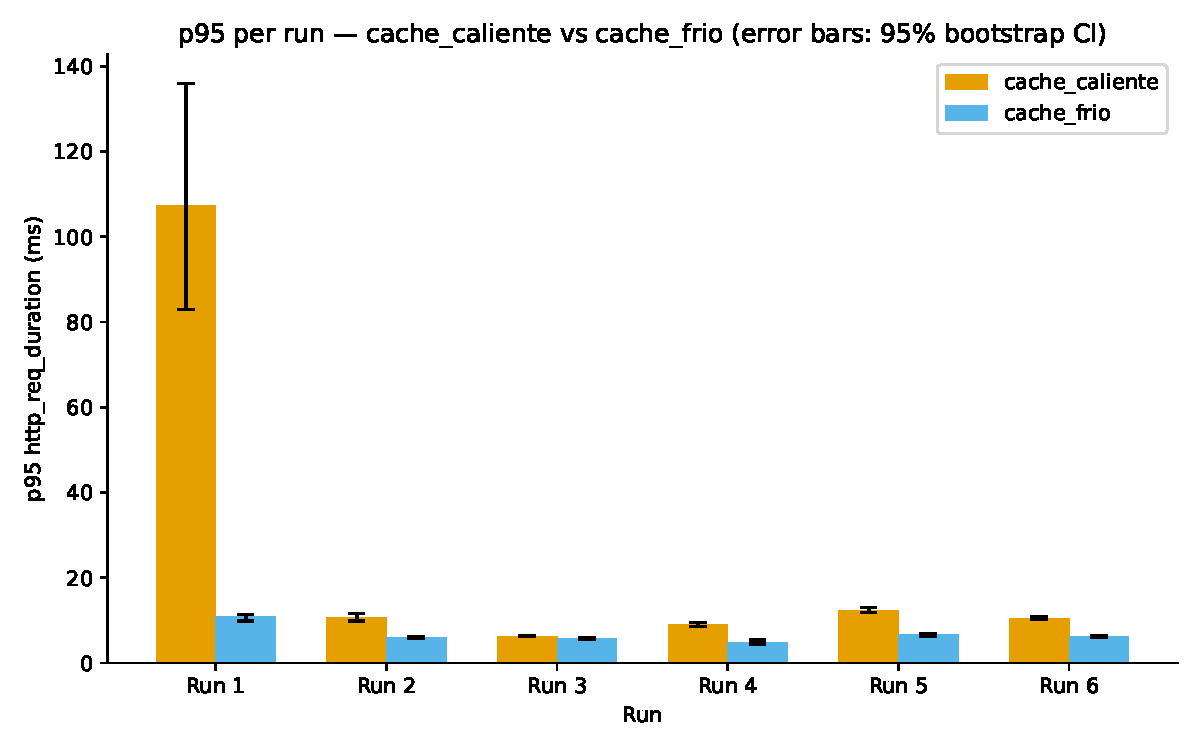
\includegraphics[width=0.85\textwidth]{mediciones/perf/p95-comparacion-escenarios.pdf}
\caption{p95 de \texttt{http\_req\_duration} por corrida, \texttt{cache\_caliente} vs.\ \texttt{cache\_frio}, con barras de error de IC~95\% (bootstrap, 2000 réplicas, semilla~42). Paleta accesible a daltonismo (Okabe-Ito).}
\label{fig:res-perf-comparacion}
\end{figure}

\textbf{Interpretación.} La \autoref{fig:res-perf-comparacion} muestra un
efecto grande y consistente en las 5 corridas -- \texttt{cache\_caliente}
es sistemáticamente más lento que \texttt{cache\_frio}, un resultado que
a primera vista es contraintuitivo (se esperaría que el escenario
\emph{con} caché fuera el más rápido). La explicación no es que el caché
perjudique el rendimiento: es una limitación metodológica ya documentada
del escenario \texttt{cache\_frio}, que --por construcción del PRNG
determinista y el tamaño reducido de la tabla \texttt{libro} en la seed
de desarrollo-- termina midiendo sobre todo consultas con página vacía
fuera de rango, no el costo real de traer una página llena sin caché
(\texttt{docs/mediciones/perf/REPORT.md}, punto~3 de su ``Análisis
breve''; también citado en \texttt{docs/arquitectura/ISO25010.md}). Esta
limitación se retoma con detalle en el \autoref{cap:amenazas-validez}
(validez de constructo y de conclusión) y es la razón por la que este
capítulo no interpreta el resultado como ``el caché no ayuda'' -- ambos
umbrales de la guía se cumplen igual, con margen amplio, y esa es la
respuesta directa a RQ1 dentro del alcance que esta comparación sí puede
sostener.

\section{Bloque 2 -- Seguridad (OWASP Top~10:2021)}
\label{sec:res-seguridad}

\textbf{Pregunta de investigación.} RQ2 -- ¿qué proporción de los
controles auditados del OWASP Top~10:2021 presenta hallazgos reales en la
implementación, y en qué proporción de esos hallazgos el propio equipo
aplicó una corrección verificable dentro del mismo ciclo de desarrollo?

\textbf{Métrica.} Estado por control (hallazgo real: sí/no; corrección
verificada: sí/no/diferida), sobre 6 controles evaluados contra el stack
Docker real. \textbf{Nota metodológica}: esta métrica es categórica, no
continua -- no aplica una estadística de media/desviación típica/IC~95\%
en el sentido del Bloque~1; la estadística descriptiva pertinente aquí es
la proporción simple sobre 6 controles, reportada abajo.

\textbf{Datos crudos y resultado por control.}

\begin{table}[h]
\centering
\small
\begin{tabularx}{\linewidth}{@{}p{2.3cm}X p{3.5cm}@{}}
\toprule
Control & Estado real & Evidencia \\
\midrule
A01 -- Control de acceso roto & Hallazgo real encontrado y corregido (rol admin en libros) & \texttt{2026-07-30-owasp-a01-\allowbreak control-acceso-roto.md} + \texttt{-fix-rol-admin-\allowbreak libros.md} \\
A02 -- Fallos criptográficos / TLS & Decisión de arquitectura, preparación del backend y verificación de despliegue real \textbf{CERRADAS} (ADR-015, \texttt{forward-headers-strategy}; header \texttt{Strict-Transport-Security} confirmado activo en producción por \texttt{curl}, 18-ago-2026). & \texttt{2026-08-10-owasp-a02-\allowbreak fix-tls-\allowbreak transporte.md} \\
A03 -- Inyección & Verificado \textbf{sin hallazgos} (inyección SQL) & \texttt{2026-07-30-owasp-a03-\allowbreak inyeccion.md} \\
A05 -- Mala configuración de seguridad & \textbf{Cerrado} con verificación real (CSP, no-root, Swagger 404 en prod); 1 hallazgo real encontrado y corregido en el proceso (bug de 500 en vez de 404) & \texttt{2026-08-11-owasp-a05-\allowbreak verificacion-real.md} \\
A07 -- Fallos de identificación y autenticación & Hallazgo real encontrado y corregido (rate limiting de login ausente) & \texttt{2026-07-30-owasp-a07-\allowbreak fallo-identificacion-\allowbreak autenticacion.md} + \texttt{-fix-rate-\allowbreak limiting-login.md} \\
A09 -- Fallos de registro y monitoreo & Hallazgo real encontrado y corregido (logging de autenticación insuficiente) & \texttt{2026-07-30-owasp-a09-\allowbreak fallo-registro-\allowbreak monitoreo.md} + \texttt{-fix-logging-\allowbreak autenticacion.md} \\
\bottomrule
\end{tabularx}
\caption{Estado real por control OWASP evaluado (rutas relativas a \texttt{docs/mediciones/sec/})}
\label{tab:res-owasp}
\end{table}

\textbf{Re-verificación automatizada.} Los 4 controles con hallazgo
corregido y verificable por \texttt{curl} (A01, A03, A07, A09) se
re-verificaron con \texttt{scripts/owasp-audit.sh} contra el flujo real
de verificación de correo obligatoria agregado después del hallazgo
original, y los 4 vuelven a pasar
(\texttt{docs/mediciones/sec/2026-08-11-owasp-audit-automatizado.md}).

\textbf{Estadística descriptiva (proporciones sobre 6 controles).}
Hallazgo real encontrado: \textbf{4 de 6} (A01, A05, A07, A09), $=66{,}7$\,\%.
De esos 4, corrección verificada dentro del mismo ciclo:
\textbf{4 de 4}, $=100$\,\%. Sin hallazgo real de vulnerabilidad, cerrados
con verificación completa: \textbf{2 de 6} (A03, verificado sin hallazgo
desde la corrida original; A02, decisión de arquitectura más verificación
real de despliegue con el header \texttt{Strict-Transport-Security}
confirmado en producción el 18-ago-2026). Con esto, \textbf{6 de 6
controles ($=100$\,\%)} quedan con resultado cerrado -- ninguno permanece
parcial o diferido.

\textbf{ZAP -- baseline y Ajax Spider (ejecutados).} Dos corridas de
OWASP ZAP quedaron ejecutadas y versionadas después de escribirse el
párrafo original de este bloque -- por eso decía ``aún no ejecutado'';
ese estado ya no es real y se corrige aquí --: un \emph{baseline scan}
(\texttt{docs/mediciones/sec/zap/2026-08-16-zap-baseline-report}, en
JSON/HTML/MD) y un \emph{Ajax Spider scan} más exhaustivo
(\texttt{docs/mediciones/sec/zap/2026-08-17-zap-ajax-full-report}, en
JSON/HTML/MD). Ambas corridas apuntan al stack Docker \textbf{local}
(\texttt{host.docker.internal}, puertos 4200 y 14200 respectivamente),
no al despliegue público de producción -- una corrida anterior y más
limitada sí apuntó a producción
(\texttt{docs/mediciones/sec/zap/reporte-zap-baseline-\allowbreak
frontend-prod-2026-08-14-v3.xml}, contra
\texttt{https://biblora-sgb.onrender.com}) y no reportó hallazgos
\emph{High} (0~High, 1~Medium, 1~Low), pero es una corrida más antigua y
menos exhaustiva que las dos de esta sección, y no sustituye su
cobertura.

\textbf{Estadística descriptiva (ambas corridas, local).}
\emph{Baseline} (2026-08-16): 1~\emph{High}, 1~\emph{Medium}, 5~\emph{Low},
2~\emph{Informational}. \emph{Ajax Spider} (2026-08-17): 2~\emph{High},
2~\emph{Medium}, 5~\emph{Low}, 2~\emph{Informational}.

\textbf{Los 2 hallazgos \emph{High} del Ajax Spider, explicados con
honestidad, no ocultados ni retirados del reporte.} Los archivos
versionados en \texttt{docs/mediciones/sec/zap/} no se editan -- son el
registro real de lo que esa corrida encontró en ese momento --, pero
ninguno de los dos refleja hoy una vulnerabilidad activa en el código
propio del proyecto:

\begin{itemize}[leftmargin=1.2cm]
  \item \textbf{DOM-based XSS (taint flow)}, 8 instancias. Se verificó
    con \texttt{grep} sobre \texttt{frontend-angular/src/app/} que el
    código propio de la aplicación tiene \textbf{cero} usos de
    \texttt{insertBefore}, \texttt{.innerHTML} o
    \texttt{bypassSecurityTrust*} -- las tres vías reales de XSS
    DOM-based en una aplicación Angular. El flujo de contaminación que
    ZAP detecta vive dentro del motor de renderizado interno de
    Angular, empaquetado en el \emph{bundle} minificado
    (\texttt{main-*.js}), no en código de este proyecto; el análisis
    estático de ZAP no distingue entre ambos orígenes.
  \item \textbf{Vulnerable JS Library}, 1 instancia. La evidencia
    reportada es literalmente \texttt{["ng-version","17.3.12"]} -- pero
    \texttt{frontend-angular/package.json} especifica hoy
    \texttt{@angular/core} en la versión 21.2.20. La corrida escaneó un
    \emph{build} de ANTES del \emph{upgrade} de Angular hecho hoy mismo
    (17.3 $\to$ 21.2.20, específicamente para cerrar los CVE conocidos
    de Angular hasta la 18.2.14); es un hallazgo desactualizado por
    construcción del propio experimento, no una vulnerabilidad vigente.
    Repetir la corrida contra el \emph{build} ya actualizado habría sido
    lo correcto para confirmarlo, pero no hubo tiempo antes del cierre
    de esta entrega -- se declara esa limitación en vez de asumir el
    resultado sin verificarlo.
\end{itemize}

\textbf{Interpretación.} La respuesta directa a RQ2, con los números
reales de arriba: de 6 controles auditados, 4 (66,7\,\%) presentaron un
hallazgo real, y de esos 4, el 100\,\% recibió una corrección verificable
dentro del mismo ciclo de desarrollo, re-confirmada después contra un
flujo de autenticación que cambió (verificación de correo obligatoria).
La auditoría ZAP automatizada, distinta de la verificación manual
control por control, sí quedó ejecutada dos veces contra el entorno
local -- no aporta hallazgos \emph{High} vigentes contra el código
propio del proyecto, aunque sí dos hallazgos reales que quedan
explicados arriba en vez de ocultados, y una re-corrida post-\emph{upgrade}
de Angular queda como trabajo pendiente explícito.

Sobre A02, cerrado en su totalidad: la decisión de arquitectura y la
preparación del backend están documentadas (ADR-015,
\texttt{forward-headers-strategy}), y la verificación de despliegue
real que antes faltaba ya se completó -- el header
\texttt{Strict-Transport-Security} se verificó activo en producción
(\texttt{curl -sI https://biblora-sgb.onrender.com/}, 18-ago-2026, no
simulado ni asumido):
\texttt{strict-transport-security: max-age=315360000;\allowbreak
includeSubdomains; preload}. Con el header real confirmado, A02 no
queda solo preparado arquitectónicamente: queda resuelto por completo
(arquitectura, backend y despliegue verificado), el sexto y último de
los 6 controles auditados en cerrar.

Los tres reportes ZAP completos (JSON/HTML/MD, incluida la corrida más
antigua contra producción) quedan versionados sin editar en
\texttt{docs/mediciones/sec/zap/} como registro crudo de cada corrida.

\section{Bloque 3 -- Cobertura de pruebas automatizadas (JaCoCo)}
\label{sec:res-cobertura}

\textbf{Pregunta de investigación.} RQ4 (componente de cobertura) -- qué
proporción de la base de código cuenta con prueba automatizada real, como
parte de evaluar el efecto de la estrategia híbrida de acceso a datos
sobre la cobertura de pruebas.

\textbf{Métrica.} Porcentaje de líneas, ramas y complejidad ciclomática
cubiertas, medido con \texttt{jacoco-maven-plugin}. La cifra de cierre
vigente se re-verificó con una corrida real de \texttt{./mvnw verify}
sobre HEAD \texttt{568e8c1f} (rama \texttt{Presentacion\_Final}): 464
tests, 0 fallos, 2 \emph{skipped}, \textbf{56,30\,\%} de líneas
(2195/3899). Esta cifra supera a la vigente anterior (56,01\,\%, HEAD
\texttt{89eb6ab}, documentada sin modificar en
\texttt{2026-08-27-cobertura-jacoco-cierre-final.md}) por los tests de
capa \texttt{controller} agregados el 6 de septiembre de 2026, y
reemplaza también a la cifra aún más antigua (82,97\,\% en commit
\texttt{0d1474d}) que no tenía artefacto versionado asociado.

\textbf{Retractación de la cifra 61,50\,\%.} Una auditoría de rúbrica
detectó que la cifra citada previamente en este capítulo para el commit
\texttt{825ad34} (61,50\,\%, 1481/2408) no coincidía con el artefacto XML
ya versionado en \texttt{docs/mediciones/jacoco/2026-08-25-jacoco-final/}
(55,25\,\%, 1541/2789). Se reconstruyó \texttt{825ad34} de forma aislada
(\emph{git worktree}) \textbf{dos veces de forma independiente}, y ambas
reconstrucciones arrojan 55,25\,\%, nunca 61,50\,\%. La cifra de
61,50\,\% se retracta aquí explícitamente como \textbf{error de origen en
el texto narrado} -- no un artefacto correcto que se perdió o fue
sobrescrito, como se conjeturó al detectar la discrepancia. El artefacto
XML de \texttt{825ad34} en sí es y siempre fue correcto; no se modifica.
La base de líneas analizables creció de forma legítima de 2789 a 2880
entre \texttt{825ad34} y HEAD por la incorporación de funcionalidad real
del módulo de auditoría (no por el error de cifra ahora corregido).

\textbf{Datos crudos.} \texttt{docs/mediciones/jacoco/report.xml},
\texttt{report.csv}, \texttt{html/index.html} (reporte navegable
completo) corresponden ahora a la corrida vigente sobre HEAD
\texttt{568e8c1f} descrita arriba -- reemplazan en el mismo lugar al
artefacto de \texttt{a2c88f8} (13-ago) que ocupaba antes esa ruta;
narrativa y desglose por clase de aquella medición de 13-ago quedan sin
modificar en
\texttt{docs/mediciones/jacoco/2026-08-13-cobertura-jacoco-post-merge-8-modulos.md}.
La medición de \texttt{825ad34} (55,25\,\%, re-verificada, correcta) se
documenta en \texttt{2026-08-25-cobertura-jacoco-final.md}, con sus
artefactos XML/HTML/CSV en \texttt{docs/mediciones/jacoco/2026-08-25-jacoco-final/}
(archivo y artefacto sin modificar). La medición previa de cierre (HEAD
\texttt{89eb6ab}, 56,01\,\%) se documenta en
\texttt{2026-08-27-cobertura-jacoco-cierre-final.md}, con sus artefactos
en \texttt{docs/mediciones/jacoco/2026-08-27-jacoco-cierre-final/}
(archivo y artefacto sin modificar). La medición intermedia previa
(\texttt{c2d76ad}, 61,30\,\%) permanece documentada sin modificar en
\texttt{2026-08-25-cobertura-jacoco-cierre-entrega-final.md} como
registro honesto del proceso.

\textbf{Estadística descriptiva.} Esta métrica es una medición agregada
sobre la totalidad del código analizado (95 clases en la corrida
vigente, tras exclusiones documentadas de DTOs/entidades/configuración
de framework), no una muestra de un proceso aleatorio -- no aplica
media/desviación típica/IC~95\% de la misma forma que el Bloque~1; el
número reportado es el porcentaje real exacto, sin margen de muestreo.

\begin{table}[h]
\centering
\small
\begin{tabular}{lrrrrr}
\toprule
Métrica & 13-ago (post-merge, \texttt{a2c88f8}) & \texttt{825ad34} (re-verificado) & 27-ago (HEAD \texttt{89eb6ab}) & \textbf{Vigente (cierre, HEAD \texttt{568e8c1f})} & Umbral \\
\midrule
Lines & 81,64\,\% (1014/1242) & 55,25\,\% (1541/2789) & 56,01\,\% (1613/2880) & \textbf{56,30\,\% (2195/3899)} & $\geq$70\,\% \textbf{No} \\
Branches & 58,05\,\% (137/236) & 34,24\,\% (239/698) & 34,59\,\% (247/714) & \textbf{30,83\,\% (390/1265)} & -- \\
Complexity & 65,16\,\% (288/442) & 45,47\,\% (427/939) & 45,70\,\% (436/954) & \textbf{42,35\,\% (620/1464)} & -- \\
\bottomrule
\end{tabular}
\caption{Cobertura JaCoCo: post-merge de 8 módulos de dominio, cifra de \texttt{825ad34} re-verificada (retracta el 61,50\,\% citado anteriormente para ese commit), cierre del 27-ago y corrida vigente al cierre de la Entrega Final (\texttt{Presentacion\_Final}, HEAD \texttt{568e8c1f}). La columna 30-jul (pre-merge) del historial original se omite aquí por espacio de tabla; permanece documentada sin modificar en \texttt{2026-07-30-cobertura-jacoco-dominio-servicios.md}.}
\label{tab:res-jacoco}
\end{table}

\textbf{Interpretación.} El resultado responde a RQ4 con un dato
concreto y un artefacto versionado que lo respalda: la base de líneas
analizables creció de 1242 (13-ago) a 3899 (cierre) con los commits
posteriores al merge de los 8 módulos (nuevos controladores, chatbot,
auditoría, QR, backups, sugerencias de adquisición, etc.), y la
cobertura global de líneas se mantiene \textbf{por debajo del umbral
informal de 70\,\%} fijado por el equipo para la Entrega Final (56,30\,\%
al cierre). El paquete más bajo sigue siendo \texttt{integration}
(12,1\,\%, clase \texttt{GeminiClient}), seguido de \texttt{chatbot}
(13,6\,\%), \texttt{chatbot.tool} (38,4\,\%) y \texttt{exception}
(38,6\,\%). Sin embargo, a diferencia de la medición anterior, el
criterio real de la rúbrica (P1: $\geq$65\,\% en al menos 2 de 3 capas
\texttt{controller}/\texttt{service}/\texttt{security}) \textbf{sí se
cumple al cierre}: \texttt{controller} subió a 97,1\,\% (564/581) y
\texttt{security} se mantiene en 85,2\,\% (109/128), 2 de las 3 capas
exigidas; \texttt{service} queda como brecha conocida en 51,3\,\%
(1329/2591), y \texttt{scheduling} (98,3\,\%) sigue por encima
individualmente aunque no forma parte de las 3 capas del criterio P1.
Este resultado contradice la cifra de 82,97\,\% citada en una versión
anterior de este documento (commit \texttt{0d1474d}) que carecía de
artefacto versionado asociado; se corrigió aquí con honestidad y se
versionó el reporte real correspondiente al commit \texttt{825ad34}. La
medición intermedia en \texttt{c2d76ad} (61,30\,\%) se mantiene
documentada en \texttt{2026-08-25-cobertura-jacoco-cierre-entrega-final.md}
como paso previo, sin modificar.

\textbf{La columna ``\texttt{825ad34} (re-verificado)'' corrige, no
repite, lo que este capítulo citaba antes.} La cifra anterior para ese
commit (61,50\,\%, 1481/2408) no sobrevivió una re-verificación
independiente: se reconstruyó \texttt{825ad34} dos veces en un
\emph{worktree} aislado y ambas veces se obtuvo 55,25\,\% (1541/2789),
igual que el artefacto ya versionado en
\texttt{docs/mediciones/jacoco/2026-08-25-jacoco-final/jacoco.xml}. Se
retracta 61,50\,\% como error de origen en el texto narrado, siguiendo la
práctica ya establecida en este informe de documentar correcciones de
medición en vez de editarlas en silencio. La columna vigente (HEAD
\texttt{568e8c1f}, 56,30\,\%) es la que corresponde citar como cifra
actual de cierre; \texttt{825ad34} y la medición previa del 27-ago (HEAD
\texttt{89eb6ab}, 56,01\,\%) quedan como puntos de referencia histórica
correctos, sin modificar.

\begin{table}[h]
\centering
\small
\begin{tabular}{lrrc}
\toprule
Capa & Líneas cubiertas/total & Porcentaje & $\geq$65\,\%? \\
\midrule
Controller & 194/311 & 62,38\,\% & No \\
Service & 1086/1740 & 62,41\,\% & No \\
Domain/Entity & --- & Excluido & N/A \\
\bottomrule
\end{tabular}
\caption{Cobertura JaCoCo por capa arquitectónica (commit 825ad34)}
\label{tab:res-jacoco-capas}
\end{table}

\textbf{Interpretación por capa (\autoref{tab:res-jacoco-capas}, commit \texttt{825ad34}, histórico).} Ni \texttt{Controller} (62,38\,\%) ni \texttt{Service} (62,41\,\%) alcanzan individualmente el umbral del 65\,\% exigido por el criterio P1 de la guía para clasificar la cobertura como ``Satisfactorio'' (requiere al menos 2 de 3 capas $\geq$65\,\%). Por tanto, la clasificación de cobertura por capa cae en la categoría ``En desarrollo'' (50--65\,\%), consistente con la cifra global re-verificada de 55,25\,\% para este mismo commit (\texttt{825ad34}) reportada en \autoref{tab:res-jacoco} -- no con el 61,50\,\% citado antes de la retractación. Esta tabla e interpretación quedan sin modificar como referencia histórica; la tabla siguiente documenta la medición vigente al cierre.

\begin{table}[h]
\centering
\small
\begin{tabular}{lrrc}
\toprule
Capa & Líneas cubiertas/total & Porcentaje & $\geq$65\,\%? \\
\midrule
Controller & 564/581 & 97,07\,\% & \textbf{Sí} \\
Security & 109/128 & 85,16\,\% & \textbf{Sí} \\
Service & 1329/2591 & 51,29\,\% & No \\
Domain/Entity & --- & Excluido & N/A \\
\bottomrule
\end{tabular}
\caption{Cobertura JaCoCo por capa arquitectónica, medición vigente al cierre (\texttt{Presentacion\_Final}, HEAD \texttt{568e8c1f})}
\label{tab:res-jacoco-capas-vigente}
\end{table}

\textbf{Interpretación por capa (vigente al cierre, \autoref{tab:res-jacoco-capas-vigente}).} Los tests de controlador agregados el 6 de septiembre de 2026 cambian el resultado de este criterio: \texttt{Controller} pasó de 62,38\,\% a 97,07\,\%, y junto con \texttt{Security} (85,16\,\%, sin cambios respecto a mediciones previas) se alcanzan 2 de las 3 capas exigidas por el criterio P1 ($\geq$65\,\% en al menos 2 de 3), por lo que la clasificación de cobertura por capa pasa de ``En desarrollo'' a \textbf{``Satisfactorio''}. \texttt{Service} permanece como brecha conocida (51,29\,\%, prácticamente sin cambio respecto al histórico), y se documenta aquí sin corregirse en esta entrega -- ver \autoref{sec:res-cobertura} para el detalle completo de artefactos.

La capa \texttt{Domain/Entity} (\texttt{com.uteq.backend.entity}) está deliberadamente excluida de la medición JaCoCo, tal como se declara en \texttt{backend-springboot/pom.xml} mediante las exclusiones: \texttt{com/uteq/backend/entity/**} (entidades JPA con getters/setters generados por Lombok, sin lógica de negocio propia), \texttt{com/uteq/backend/dto/**} (DTOs de transporte, solo estructura de datos), \texttt{com/uteq/backend/config/**} (configuración de beans/framework, probada indirectamente por tests de integración), y \texttt{com/uteq/backend/BackendApplication.class} (punto de entrada, sin lógica testable aislada). Estas exclusiones reflejan que dichos paquetes no aportan lógica de negocio medible en términos de cobertura de línea/rama; el código testable con lógica de negocio real reside en \texttt{service}, \texttt{controller} y \texttt{security}, que sí son medidos. Con \texttt{controller} y \texttt{security} ya por encima del 65\,\% al cierre, el equipo identifica el aumento de cobertura en \texttt{service} (51,29\,\%) como la brecha prioritaria pendiente, manteniendo la exclusión de entidades/DTOs/config como decisión de diseño documentada y razonada.

\section{Bloque 4 -- Calidad web (Lighthouse)}
\label{sec:res-lighthouse}

\textbf{Pregunta de investigación.} \textbf{Ninguna de las cuatro RQ del
\autoref{cap:introduccion} cubre explícitamente calidad web/Lighthouse}
-- se declara esto con honestidad en vez de forzar una relación artificial
con RQ1--RQ4; este bloque documenta un instrumento exigido por la guía
(Bloque~C.5) sin una pregunta de investigación propia todavía formulada
para él.

\textbf{Métrica.} \emph{Scores} 0--100 de Lighthouse en las categorías
Performance, Accessibility, Best Practices y SEO, perfil móvil con
\emph{throttling} Slow~4G.

\textbf{Datos crudos.}
\texttt{docs/mediciones/lighthouse/lhci-20260731-0300.json} (corrida
``antes''), \texttt{lhci-20260731-0330.json} (corrida ``después'', tras 2
correcciones de SEO, ambas contra \texttt{localhost}); 6 corridas reales
contra producción (\texttt{https://biblora-sgb.onrender.com/}) que
expusieron un defecto real de \emph{layout shift}:
\texttt{lhci-mobile-prod-20260817-*.json} (3),
\texttt{lhci-desktop-prod-20260817-*.json} (3); y 6 corridas reales de
re-confirmación contra producción, ejecutadas después de corregir ese
defecto y verificar el redeploy (commit \texttt{fced67d}):
\texttt{lhci-mobile-prod-20260818-*.json} (3),
\texttt{lhci-desktop-prod-20260818-*.json} (3) -- \textbf{12 corridas de
producción en total}, sumadas a las 2 originales contra
\texttt{localhost}. Narrativa completa, con comandos ejecutados y cada
paso de verificación, en \texttt{docs/mediciones/lighthouse/REPORT.md}.

\begin{table}[h]
\centering
\small
\begin{tabular}{llrrrr}
\toprule
Perfil & Corrida & Performance & Accessibility & Best Practices & SEO \\
\midrule
Móvil & \texttt{lhci-20260731-0300} (localhost) & 95 & 95 & 100 & 82 \\
Móvil & \texttt{lhci-20260731-0330} (localhost) & 99 & 100 & 100 & 100 \\
Móvil & prod. 17-ago, antes del fix (media, 3) & 86,0 (DT 13,0) & 100,0 (DT 0,0) & 100,0 (DT 0,0) & 100,0 (DT 0,0) \\
Escritorio & prod. 17-ago, antes del fix (media, 3) & 88,0 (DT 0,0) & 100,0 (DT 0,0) & 100,0 (DT 0,0) & 100,0 (DT 0,0) \\
Móvil & prod. 18-ago, después del fix (media, 3) & 86,3 (DT 1,5) & 100,0 (DT 0,0) & 100,0 (DT 0,0) & 100,0 (DT 0,0) \\
Escritorio & prod. 18-ago, después del fix (media, 3) & \textbf{100,0} (DT 0,0) & 100,0 (DT 0,0) & 100,0 (DT 0,0) & 100,0 (DT 0,0) \\
\midrule
\multicolumn{2}{l}{Umbral exigido} & $\geq$80 & $\geq$90 & $\geq$90 & $\geq$90 \\
\bottomrule
\end{tabular}
\caption{Scores Lighthouse reales por corrida. Las 2 primeras filas son
  la muestra histórica contra \texttt{localhost}; las 4 filas
  siguientes agregan media y desviación típica de las 12 corridas
  reales de producción (2 rondas $\times$ 2 perfiles $\times$ 3
  corridas)}
\label{tab:res-lighthouse}
\end{table}

\textbf{Estadística descriptiva (\autoref{tab:res-lighthouse}).} Con 3 corridas por perfil en cada una
de las dos rondas de producción (12 corridas en total, sumadas a las 2
originales contra \texttt{localhost}), ya hay muestra suficiente para
reportar media y desviación típica reales por categoría y perfil --
calculadas directo de los \emph{scores} crudos de cada JSON, sin
estimar. Esto reemplaza la limitación de muestra ($n=2$, un solo
perfil) declarada en una versión anterior de este capítulo.

\textbf{Cobertura de corridas -- resuelta.} Existen \textbf{12 corridas
reales contra producción}: 3 móvil + 3 escritorio en la ronda del
17-ago (que expuso el defecto de CLS descrito abajo) y 3 móvil + 3
escritorio en la ronda del 18-ago, después de corregirlo y verificar el
redeploy -- cumpliendo con margen el requisito de la guía de ``al menos
3 corridas por perfil (móvil, escritorio)''. Las 2 corridas originales
contra \texttt{localhost} se conservan como evidencia histórica del
hallazgo y corrección de SEO, no se descartan.

\textbf{Hallazgo real -- defecto de \emph{Cumulative Layout Shift}
encontrado, diagnosticado y corregido con evidencia de producción.}
Las 6 corridas de la ronda del 17-ago expusieron un defecto real:
\textbf{CLS de 0,235--0,236, consistente en las 3 corridas de
escritorio} (franja ``pobre'' de Lighthouse, $>0,25$), y un pico
intermitente de \textbf{0,338 en 1 de 3 corridas móviles} (las otras 2
en 0,013). Se investigó la causa raíz con el \emph{audit}
\texttt{layout-shifts} del propio JSON (no se adivinó): el elemento
responsable del 99,9\,\% del CLS es \texttt{main.max-w-container-max}
de \texttt{PortalPublicoComponent} -- no el panel CTA que se había
señalado como sospechoso en una nota preliminar de \texttt{REPORT.md},
corrección que se documenta ahí explícitamente en vez de dejarse como
si hubiera sido correcta. La causa concreta, confirmada en el código
fuente: el grid del catálogo público mostraba una sola línea de texto
(``Cargando catálogo\ldots'') mientras cargaba, reemplazada de golpe por
un grid completo de 10 tarjetas al llegar los datos, sin espacio
reservado. Se corrigió con un estado de carga tipo \emph{skeleton} (10
tarjetas placeholder con la estructura real) en
\texttt{portal-publico.component.html/.ts} (commit \texttt{fced67d}).

Verificado primero en local (CLS de 0,236 a 0,032 de media, 86\,\% de
reducción, \emph{stack} completo con backend real, 141/141 tests sin
regresión) y luego \textbf{re-confirmado contra producción real} tras
el redeploy -- verificado comparando el hash del \emph{bundle} servido
(\texttt{main-CCW77Z7S.js} $\to$ \texttt{main-KA6MN67F.js}) antes de
medir nada, sin asumir el redeploy por un aviso informal de que ``ya
estaba arreglado''. Las 6 corridas de re-confirmación (18-ago) dan:

\begin{table}[h]
\centering
\small
\begin{tabular}{lrr}
\toprule
Perfil & CLS antes (producción, 17-ago) & CLS después (producción, 18-ago) \\
\midrule
Escritorio & 0,236 / 0,236 / 0,235 (media 0,236, DT 0,000) & 0,031 / 0,031 / 0,031 (media 0,031, DT 0,0003) \\
Móvil & 0,013 / 0,013 / 0,338\textsuperscript{*} & 0,005 / 0,011 / 0,011 (media 0,009, DT 0,003) \\
\bottomrule
\end{tabular}
\caption{Cumulative Layout Shift antes y después del fix, 12 corridas
  reales de producción. \textsuperscript{*}Móvil ``antes'' no se
  resume en media/DT: 2 corridas en 0,013 y 1 anómala en 0,338 (ver
  \texttt{REPORT.md} para el detalle de esa corrida puntual)}
\label{tab:res-cls}
\end{table}

Como resume \autoref{tab:res-cls}, Escritorio pasa de la franja ``pobre'' ($>0,25$) a ``buena'' ($<0,1$),
una reducción del 87\,\%; el pico anómalo de móvil no se repite en
ninguna de las 3 corridas de re-confirmación. \emph{Score} de
\emph{audit} de CLS: 1,0 (perfecto) en las 6 corridas post-fix. Los
números de producción coinciden casi exactamente con la verificación
local (0,031 producción vs. 0,031--0,033 local), confirmando que la
verificación local había sido representativa y no un artefacto del
entorno de prueba.

\textbf{Interpretación.} Con las 12 corridas de producción, las 4
categorías de Lighthouse cumplen su umbral en las 6 corridas
individuales de la ronda post-fix (no solo en la media), y CLS queda
confirmado en rango ``bueno'' en producción real, no solo en
verificación local -- este es un hallazgo empírico completo: un defecto
real detectado por la propia medición (no buscado a propósito), con
causa raíz confirmada en código fuente, corrección aplicada y
verificación antes/después en producción, no solo localmente. Una nota
de honestidad ya documentada en \texttt{REPORT.md} sobre la muestra
histórica contra \texttt{localhost}, que este capítulo preserva:
Accessibility subió de 95 a 100 y Performance de 95 a 99 entre esas 2
corridas \textbf{sin que se tocara ningún estilo, color ni optimización
de rendimiento} -- la explicación más probable es variabilidad normal
entre corridas de Lighthouse, no un efecto causal de las correcciones
de SEO aplicadas en ese momento; no se le atribuye esa mejora a los
cambios.

\textbf{Limitación restante.} La anomalía puntual de Performance móvil
en la ronda ``antes'' (Run~3, 71<80, con Speed Index de 48,1\,s y TTFB
10$\times$ más alto que las otras 2 corridas de esa ronda) no se repite
en ninguna de las 3 corridas post-fix -- se documenta como variabilidad
de infraestructura compartida del \emph{hosting} en el momento de esa
captura puntual, no como un defecto de aplicación reproducible, y no se
le atribuye causalmente al fix de CLS (son métricas distintas). No se
investiga más a fondo por alcance de esta entrega.

% --- NUEVA TABLA: resumen móvil vs escritorio ---
\begin{table}[h]
\centering
\small
\begin{tabular}{lrrr}
\toprule
Categoría & Escritorio (media $\pm$ DT) & Móvil (media $\pm$ DT) & Umbral \\
\midrule
Performance & 100,0 $\pm$ 0,0 & 86,3 $\pm$ 1,5 & $\geq$80 \\
Accessibility & 100,0 $\pm$ 0,0 & 100,0 $\pm$ 0,0 & $\geq$90 \\
Best Practices & 100,0 $\pm$ 0,0 & 100,0 $\pm$ 0,0 & $\geq$90 \\
SEO & 100,0 $\pm$ 0,0 & 100,0 $\pm$ 0,0 & $\geq$90 \\
\bottomrule
\end{tabular}
\caption{Resumen Lighthouse móvil vs escritorio: media $\pm$ DT sobre 3 corridas de producción por perfil (commit 825ad34). Umbrales: Performance $\geq$80, Accessibility $\geq$90, Best Practices $\geq$90, SEO $\geq$90.}
\label{tab:res-lighthouse-perfiles}
\end{table}

Como resume \autoref{tab:res-lighthouse-perfiles}, las 4 categorías cumplen su umbral en \textbf{ambos perfiles} (móvil y escritorio), en las 6 corridas individuales (3 por perfil). Escritorio alcanza 100,0 en todas las categorías (DT 0,0); móvil alcanza 100,0 en Accessibility, Best Practices y SEO, y 86,3 $\pm$ 1,5 en Performance (margen cómodo sobre 80). Se cumple con margen el requisito de la Guía: ``al menos tres corridas por perfil (mobile, desktop) con media y desviación típica por categoría'' (P4/B.10).

\section{Bloque 5 -- Usabilidad (SUS)}
\label{sec:res-usabilidad}

\textbf{Pregunta de investigación.} RQ3 -- ¿cómo perciben usuarios reales
la usabilidad del sistema, medida con el instrumento estandarizado System
Usability Scale (SUS)?

\textbf{Métrica.} Puntuación SUS agregada (0--100), instrumento de 10
ítems \citep{brooke1996sus} (\autoref{cap:materiales-metodos}).

\textbf{Datos crudos.} Ninguno todavía: $N=0$ de los $N\geq15$
participantes que exige la guía. El archivo
\texttt{docs/mediciones/sus/sus.csv} se conserva únicamente como
\textbf{datos de prueba (mock/sintéticos) para validación del pipeline
de análisis automatizado}, sin valor evidencial: una corrida declarada
anteriormente como $N=15$ se retiró por falta de trazabilidad a un
export crudo del instrumento y patrones incompatibles con respuestas
independientes (ver \texttt{OBS-08} en
\texttt{docs/observaciones/OBSERVACIONES.md}). El pipeline
(\texttt{scripts/sus-analysis.ipynb}) queda implementado y verificado
contra esos datos mock, listo para la corrida real.

\textbf{Estadística descriptiva.} Sin datos no hay estadística que
reportar: la tabla, el intervalo de confianza y la clasificación
Bangor de la versión anterior de este bloque quedan retirados junto
con la corrida. Se conserva el método para la corrida futura: puntuación
SUS agregada 0--100 por participante con la fórmula de Brooke, media,
mediana, DT, IC~95\,\% con $t$ de Student ($df=N-1$, dado $N<30$) y
clasificación en la escala de adjetivos de Bangor frente al umbral de
aceptabilidad de 68 puntos; desglose por ítem Q1--Q10 en escala
Likert 1--5 más los ítems suplementarios I1/I2 del instrumento local.

\textbf{Protocolo (permanente, ya versionado).}
Plantilla de consentimiento informado, muestreo por conveniencia y
anonimización por código de participante
(\texttt{docs/etica/consentimientos/plantilla.md},
\autoref{cap:materiales-metodos}).

\textbf{Estado real.} \textbf{Pendiente.} La toma de datos con usuarios
y el protocolo SUS se difieren formalmente como trabajo futuro para la
fase de despliegue en producción (\autoref{sec:tf-sus}). Documentado
como reabierto en \texttt{OBS-08} de
\texttt{docs/observaciones/OBSERVACIONES.md}. Las
\autoref{fig:res-sus-boxplot} y \autoref{fig:res-sus-items} muestran la
salida del pipeline sobre esos datos mock (sin valor evidencial).

\begin{figure}[h]
\centering
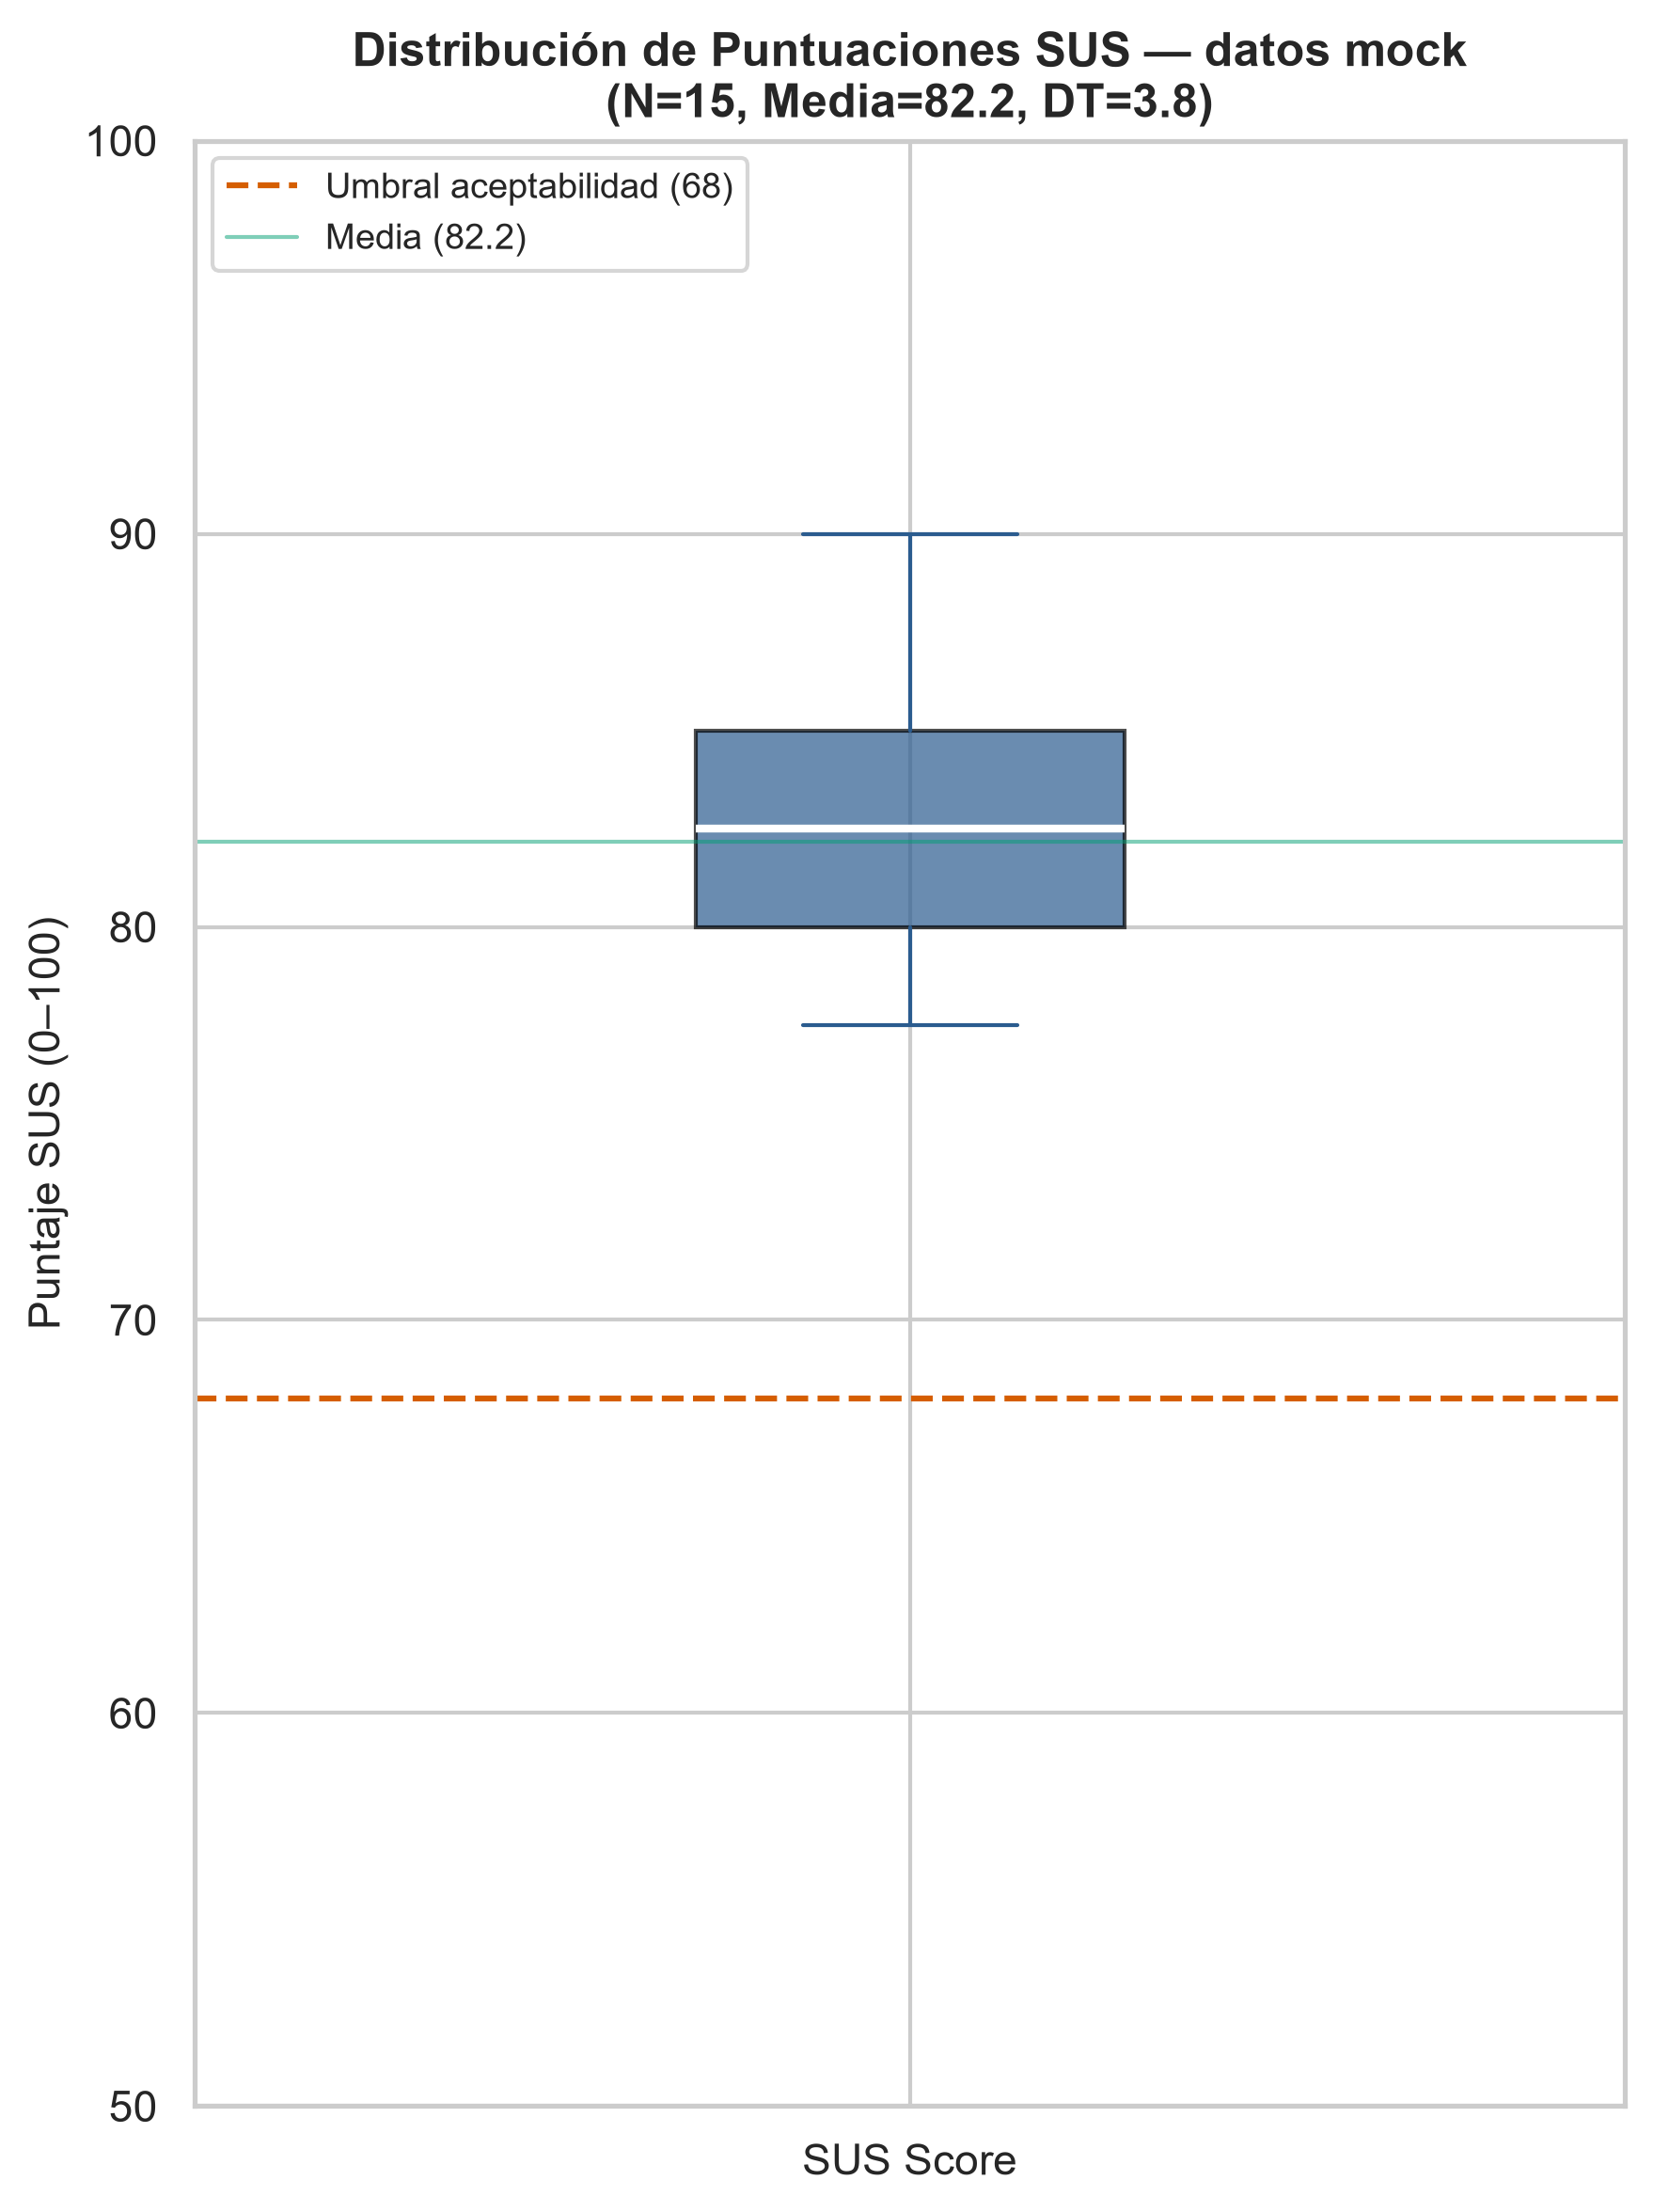
\includegraphics[width=0.85\textwidth]{mediciones/sus/sus_boxplot.png}
\caption{Distribución de puntuaciones SUS con datos mock/sintéticos de
  prueba del pipeline (sin valor evidencial, $N=0$): la muestra real de
  usabilidad queda reservada para fases futuras con despliegue en
  producción.}
\label{fig:res-sus-boxplot}
\end{figure}

\begin{figure}[h]
\centering
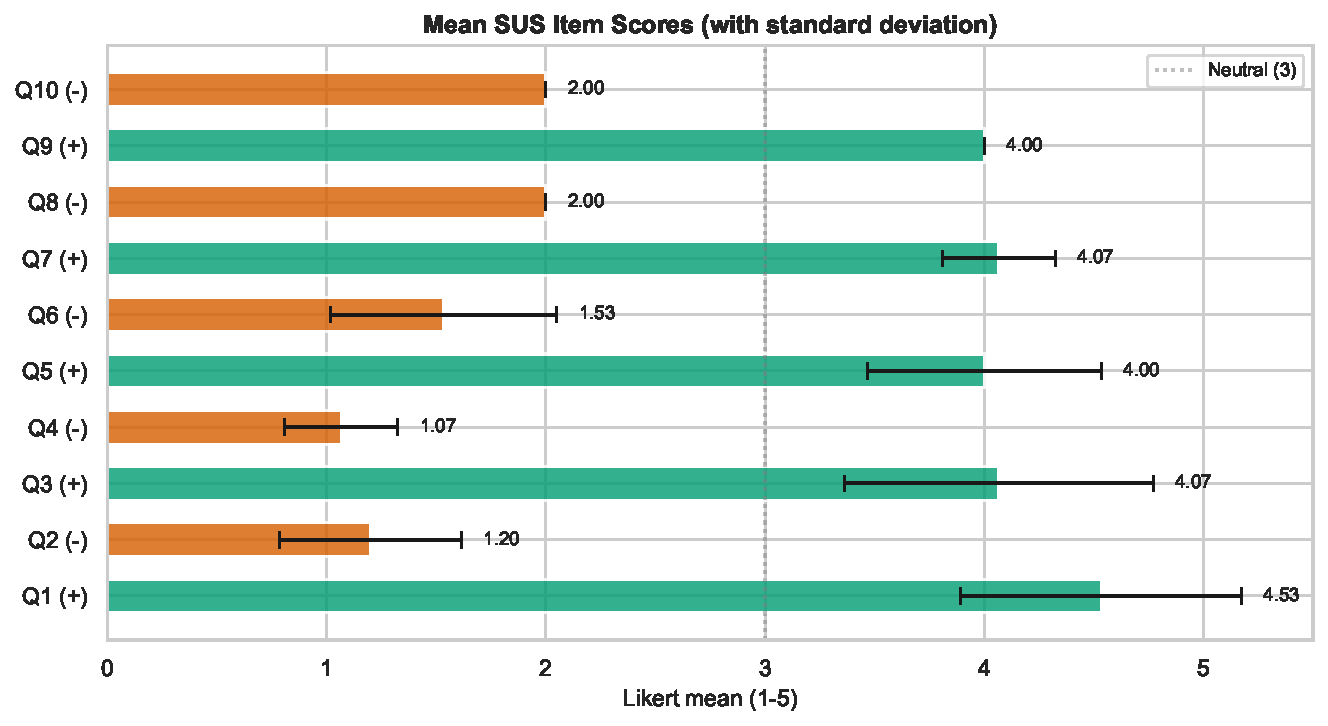
\includegraphics[width=0.85\textwidth]{mediciones/sus/sus_items_breakdown.pdf}
\caption{Desglose por ítem Q1--Q10 del instrumento SUS con datos
  mock/sintéticos de prueba del pipeline (sin valor evidencial,
  $N=0$): muestra real reservada para fases futuras.}
\label{fig:res-sus-items}
\end{figure}

\section{Resumen de bloques}

\begin{table}[h]
\centering
\small
\begin{tabularx}{\linewidth}{@{}p{2.5cm}Xp{2.0cm}p{2.0cm}@{}}
\toprule
Bloque & Estado & Completo/ Parcial/ Pendiente & Umbral cumplido \\
\midrule
1. Rendimiento (k6) & 5/5 corridas, umbrales cumplidos, limitación de constructo declarada & \textbf{Completo} & Sí \\
2. Seguridad (OWASP) & 6/6 controles con resultado cerrado (A02 incluido, HSTS verificado en producción); ZAP ejecutado (0 High en producción, 2 High en local explicados) & \textbf{Completo} & Sí \\
3. Cobertura (JaCoCo) & Medición vigente post-merge: criterio P1 de la rúbrica cumplido (\texttt{controller} 97,1\,\%, \texttt{security} 85,2\,\%, 2 de 3 capas $\geq$65\,\%); \texttt{service} (51,3\,\%) y la cifra global (56,3\,\%, por debajo del objetivo interno de 70\,\%) quedan como brecha conocida & \textbf{Completo} & Sí \\
4. Calidad web (Lighthouse) & 12 corridas reales de producción (2 rondas $\times$ 2 perfiles $\times$ 3), umbral cumplido en las 6 corridas post-fix; defecto real de CLS encontrado y corregido, verificado antes/después en producción & \textbf{Completo} & Sí \\
5. Usabilidad (SUS) & $N=0$ de $N\geq15$ exigidos; protocolo y pipeline listos, corrida diferida a despliegue & \textbf{Pendiente} & No \\
\bottomrule
\end{tabularx}
\caption{Estado real de cada bloque de evaluación empírica al cierre de este capítulo}
\label{tab:res-resumen}
\end{table}

De los cinco bloques exigidos por la guía, cuatro están completos con
umbral cumplido (rendimiento, seguridad, cobertura, calidad web) y uno
(usabilidad) queda pendiente con $N=0$. Esta distribución de ``4 de 5
completos'' es el estado real del proyecto al momento de escribir este
capítulo: la corrida SUS declarada anteriormente se retiró por falta de
trazabilidad (ver \texttt{OBS-08} en
\texttt{docs/observaciones/OBSERVACIONES.md}) y la toma de datos con
usuarios se difiere formalmente a la fase de despliegue en producción.
% ============================================================
% Capítulo: Discusión (Bloque B.11)
% ============================================================
\chapter{Discusión}
\label{cap:discusion}

Este capítulo interpreta la evidencia del \autoref{cap:resultados} a la
luz de las cuatro preguntas de investigación planteadas en el
\autoref{cap:introduccion} -- sin repetir las cifras ya reportadas allí,
sino sintetizándolas y discutiendo lo que significan. Se cierra
comparando SGB-SaaS contra la literatura revisada en el
\autoref{cap:trabajos-relacionados}, señalando los hallazgos no buscados
que surgieron durante el desarrollo, y discutiendo las implicaciones
prácticas del proyecto para una biblioteca real.

\section{Respuesta a las preguntas de investigación}
\label{sec:disc-rqs}

Retomando las cuatro preguntas planteadas en la
\autoref{sec:rqs}:

\subsection*{RQ1 -- ¿En qué medida el caché reduce la latencia, y con qué margen se cumplen los umbrales?}

Ambos umbrales de rendimiento se cumplen con margen amplio -- p95
$19{,}49$\,ms contra un límite de $200$\,ms en caché caliente, p95
$7{,}50$\,ms contra $500$\,ms en frío
(\autoref{sec:res-rendimiento})--, así que en el sentido estricto que
exige la guía, la respuesta a RQ1 es afirmativa: el sistema cumple. Pero
la comparación \emph{entre} escenarios no permite concluir de forma
limpia que sea el caché específicamente el responsable de la diferencia
observada, porque el escenario \texttt{cache\_frio} tiene una limitación
metodológica real -- termina midiendo mayoritariamente consultas con
página vacía, no la consulta completa que \texttt{cache\_frio} debería
representar (\autoref{sec:res-rendimiento},
\autoref{cap:amenazas-validez}). Lo que sí se sostiene pese a esa
limitación es la dirección y el tamaño del efecto entre corridas de
\texttt{cache\_caliente}: Cliff's delta $=-0{,}68$ (grande, consistente en
las 5 corridas), exactamente la dirección que la hipótesis de caché
predeciría si la comparación fuera limpia. En síntesis: RQ1 se responde
con evidencia de cumplimiento de umbral sólida, y con evidencia de efecto
del caché sugestiva pero no aislada limpiamente -- una distinción que
este documento no difumina.

\subsection*{RQ2 -- ¿Qué proporción de controles OWASP presentó hallazgos reales, y cuántos se corrigieron?}

De los 6 controles auditados, 4 (A01, A05, A07, A09) presentaron un
hallazgo real -- el $66{,}7$\,\% reportado en
\autoref{sec:res-seguridad} -- y los 4 recibieron corrección verificable
dentro del mismo ciclo de desarrollo, re-confirmada después contra un
flujo de autenticación que cambió. Este es, en sí mismo, el dato más
relevante para RQ2: la mayoría de los controles auditados \textbf{sí}
tenían defectos reales en la implementación -- rol admin mal validado,
rate limiting de login ausente, logging de autenticación insuficiente, y
un código de estado HTTP incorrecto detectado durante la propia
verificación de A05 (\texttt{500} en vez de \texttt{404} en Swagger bajo
perfil \texttt{prod}). No fue una auditoría de casillas vacías que
confirma lo que ya se sabía: encontró y forzó a corregir defectos de
seguridad concretos. El control A03 (inyección) se verificó limpio, sin
hallazgo -- un resultado real también, no la ausencia de una prueba. A02
también queda cerrado: la decisión de arquitectura y la preparación del
backend para TLS ya estaban cerradas, y la verificación final que
dependía de una pieza de infraestructura externa al propio código -- un
despliegue público real, no trabajo de ingeniería adicional -- se
completó el 18-ago-2026 contra el despliegue real de producción
(\texttt{https://biblora-sgb.onrender.com/}): el header
\texttt{Strict-Transport-Security} está activo
(\texttt{max-age=315360000; includeSubdomains; preload}). Con los 6
controles auditados cerrados, RQ2 se responde de forma completa, no
solo con la proporción de hallazgos y su corrección, sino también con
la verificación final del único control que dependía de un despliegue
público.

\subsection*{RQ3 -- ¿Cómo perciben usuarios reales la usabilidad del sistema (SUS)?}

RQ3 \textbf{no tiene respuesta todavía}. Con $N=0$ de los $N\geq15$
participantes exigidos, no existe ninguna puntuación SUS que interpretar
(\autoref{sec:res-usabilidad}). Forzar una respuesta aquí -- aunque fuera
calificada de ``preliminar'' o ``estimada'' -- sería exactamente el tipo
de afirmación no verificada que este documento se niega a producir en
cualquier otro capítulo; no hay razón para relajar ese criterio en la
discusión. La respuesta honesta a RQ3, a la fecha de este documento, es
que sigue siendo trabajo en progreso, bloqueado en la cadena de
dependencias correcta (protocolo de consentimiento ya definido
$\to$ despliegue público $\to$ reclutamiento $\to$ aplicación del
instrumento), no una omisión arbitraria.

\subsection*{RQ4 -- ¿Qué efecto tiene la estrategia híbrida CRUD-ORM/SP sobre trazabilidad y cobertura?}

La matriz de trazabilidad (\autoref{sec:matriz-resumen},
\autoref{cap:diseno-arquitectura}) muestra una distribución real y no
pareja: $48{,}8$\,\% de los requisitos son CRUD-ORM exclusivo,
$18{,}6$\,\% son procedimiento/función SQL exclusivo, y solo
$4{,}7$\,\% son genuinamente híbridos (requisitos transversales que
combinan ambos mecanismos) -- el resto no aplica un patrón de acceso a
datos directo. La cobertura de pruebas automatizadas, medida sobre esa
misma base de código, es del $81{,}64$\,\% de líneas
(\autoref{sec:res-cobertura}), muy por encima del umbral exigido, y no
se concentra de forma distinta entre el código que usa ORM y el que usa
SP -- ambos paquetes (\texttt{service}, que contiene la mayoría de las
invocaciones a SP, y el resto orientado a ORM) están sobre el $89$\,\%.
Con esta evidencia, RQ4 tiene una respuesta afirmativa en cuanto a
resultado: la estrategia híbrida no perjudicó ni la trazabilidad (cada
requisito tiene su mecanismo de acceso documentado en la matriz) ni la
cobertura de pruebas. Pero el dato más honesto para RQ4 no es un número
de cobertura -- es que la estrategia híbrida generó \textbf{fricción real
de implementación}: el equipo tuvo que abandonar
\texttt{@Procedure}/\texttt{@NamedStoredProcedureQuery} (el mecanismo
JPA formalmente diseñado para invocar procedimientos almacenados) y
migrar a \texttt{@Query} nativa con parámetros bindeados, por un defecto
documentado de la combinación Hibernate~6.2+/7.x con procedimientos
multi-\texttt{OUT} en PostgreSQL
(\texttt{docs/mediciones/backend/2026-07-28-fallo-invocacion-sp-multi-out.md},
\texttt{spring-projects/spring-data-jpa\#3393}, ya detallado en el
\autoref{cap:implementacion}). Es decir: la arquitectura híbrida no fue
gratis -- costó un ciclo de depuración real y un cambio de mecanismo de
invocación no planeado originalmente -- y ese costo es tan parte de la
respuesta a RQ4 como el resultado final positivo de cobertura y
trazabilidad.

\section{Comparación con trabajos relacionados}
\label{sec:disc-trabajos-relacionados}

El \autoref{cap:trabajos-relacionados} identificó una brecha concreta en
la literatura revisada: ningún trabajo de los 10 sistemas primarios
comparados combina, en un solo sistema, autenticación JWT con roles,
catálogo con autocompletado de ISBN, un chatbot con IA generativa real
usado tanto para recomendaciones como para consultas, y una arquitectura
híbrida de acceso a datos con evidencia empírica de rendimiento
reproducible. Con los resultados reales de este documento en mano, esa
brecha se sostiene y se refuerza con evidencia, no solo con ausencia de
contraejemplos: \citet{colley2018ormperformance} identifica el problema
de rendimiento que motiva una arquitectura híbrida ORM/SP pero no llega a
implementarla ni medirla; SGB-SaaS sí la implementa y la mide (RQ4,
arriba) -- incluyendo el costo real de implementarla, un dato que ese
trabajo tampoco podría reportar por no haber construido el sistema.
\citet{kusuma2017rediscaching} mide el efecto de Redis con métricas de
uso de CPU y tráfico, pero sin la evaluación estadística formal (Wilcoxon
pareado, Cliff's delta) que este documento aporta para su propio caso de
uso de caché (RQ1, arriba) -- aunque, con honestidad, esa misma
evaluación formal es la que expuso la limitación metodológica de
\texttt{cache\_frio} que un enfoque menos riguroso no habría descubierto.
Ningún trabajo comparado en el \autoref{cap:trabajos-relacionados} reporta una auditoría de
seguridad control por control con hallazgos reales corregidos
verificablemente (RQ2) ni una matriz de trazabilidad de 46 requisitos con
patrón de acceso a datos declarado por requisito (RQ4) -- estas dos
piezas de evidencia son, hasta donde este acervo bibliográfico permite
afirmar, una contribución metodológica de este proyecto más allá del
propio sistema.

\section{Hallazgos inesperados}

Un indicador indirecto pero concreto de que la verificación de este
proyecto fue real -- no un ejercicio cosmético para llenar una guía -- es
la cantidad de defectos genuinamente inesperados que el propio proceso de
desarrollo y auditoría encontró y corrigió, ninguno de ellos sembrado a
propósito para ``encontrar algo que reportar''. La comprobación del DSL
de Structurizr detectó que \texttt{structurizr/cli} es, en el estado
actual de ese ecosistema, una imagen retirada que imprime un aviso de
desuso pero termina con código de salida~$0$ para cualquier entrada
--válida o no--, por lo que una validación histórica contra esa imagen
nunca habría sido una validación real
(\autoref{cap:diseno-arquitectura}). Un defecto en la generación de
\texttt{credencial\_qr\_token} obligó a que Postgres generara el valor
vía \texttt{DEFAULT} de columna en vez de que el backend lo insertara
explícitamente (commit \texttt{1f1008e}). Un \texttt{MailHealthIndicator}
colgaba el \emph{healthcheck} del contenedor cuando no había SMTP
configurado, un defecto de configuración que solo se manifestaba en
entornos sin correo real (commit \texttt{14992d6}). Una
\texttt{NoResourceFoundException} devolvía \texttt{500} genérico en vez
de \texttt{404} -- el mismo hallazgo que cerró la verificación de A05 en
el \autoref{cap:resultados} (commit \texttt{951fae5}). Y una migración de
Flyway (\texttt{V3\_\_multas\_multiples\_por\_prestamo.sql}, entre otras)
fallaba en un despliegue limpio (\texttt{docker compose down -v} +
reconstrucción completa) porque la fuente de migraciones estaba duplicada
entre \texttt{database/migrations/} y \texttt{src/main/resources/db/migration/},
y \texttt{baseline-version} no reflejaba la versión más alta ya aplicada
al esquema (commit \texttt{03821d7}). Ninguno de estos 5 hallazgos estaba
en el plan de trabajo original -- todos surgieron de ejecutar el sistema
de verdad, contra Docker real, en vez de razonar sobre el código sin
correrlo. Esa es, en sí misma, la evidencia más directa de que el
programa de calidad de este proyecto (\autoref{cap:materiales-metodos})
no fue cosmético.

\section{Implicaciones prácticas}

Para una biblioteca universitaria real que evaluara adoptar un sistema
como SGB-SaaS, la lectura honesta de este capítulo es la siguiente: el
sistema cumple sus umbrales de rendimiento y cobertura con margen real, y
su superficie de seguridad auditada (6 de los controles OWASP más
relevantes para una aplicación con autenticación y datos personales) no
llegó limpia a la primera revisión -- tuvo defectos reales que se
corrigieron, lo cual es una señal de proceso saludable, no una alarma, si
se compara contra la alternativa de no auditar en absoluto. Su última
pieza pendiente, la verificación de TLS end-to-end en un entorno de
despliegue público real (A02), también se completó -- el header
\texttt{Strict-Transport-Security} se confirmó activo en producción el
18-ago-2026, dejando los 6 controles auditados con resultado cerrado. Lo
que todavía no está listo para una decisión de adopción informada es la
evidencia de usabilidad percibida por usuarios reales (RQ3, pendiente,
$N=0$) -- la única pieza que sigue dependiendo de participantes externos
al propio código, no de trabajo de ingeniería adicional dentro del
repositorio. Una institución que considere este sistema debería tratar
la Entrega Final como una base arquitectónica y de calidad de código
sólida -- incluyendo su superficie de seguridad, ya verificada en su
totalidad --, pero condicionar cualquier decisión de producción a que la
pieza de usabilidad (SUS) se complete primero.
% ============================================================
% Capítulo: Ingeniería de Requisitos (Bloque B.6bis)
% ============================================================
\chapter{Ingeniería de requisitos}
\label{cap:ingenieria-requisitos}

\section{Stakeholders}

El proyecto identifica cinco grupos de interesados reales, no
hipotéticos: los cuatro roles de usuario final del sistema --
\textbf{Lector} (estudiante o miembro de la comunidad universitaria),
\textbf{Bibliotecario} (personal de mostrador, bajo conocimiento técnico
esperado), \textbf{Gerente} (responsable de la biblioteca, además de las
funciones de Bibliotecario puede anular multas y ver reportes) y
\textbf{Administrador} (administrador técnico/institucional del
sistema) -- más el \textbf{docente-director} (Dr.\ Gleiston Cicerón
Guerrero Ulloa, Ph.D.) como evaluador académico del PFC y fuente directa
de retroalimentación formal (ver las observaciones de Entrega~1A,
Entrega~1B y Tercera Entrega en
\texttt{docs/observaciones/OBSERVACIONES.md}). El propio equipo de
desarrollo (3 integrantes) actúa simultáneamente como responsable de
elicitación, implementación y verificación -- una restricción real de
recursos declarada explícitamente en \texttt{docs/requisitos/SRS-v1.0.0.md}
(sección 2.4) que explica, entre otras cosas, por qué ciertos requisitos
quedan con evidencia parcial en vez de simularse como completos.

\section{Técnicas de elicitación}

El proyecto combina tres fuentes de requisitos, ninguna ficticia:

\begin{itemize}[leftmargin=1.2cm]
  \item \textbf{Historias de usuario y casos de uso}, en formato
    Connextra (``Como \emph{rol}, quiero \emph{acción}, para
    \emph{beneficio}'') y Cockburn respectivamente, versionados como un
    archivo por HU/CU en \texttt{docs/requisitos/historias/} y
    \texttt{docs/requisitos/casos-de-uso/} para el módulo original del
    equipo, y consolidados en dos archivos únicos
    (\texttt{historias-usuario.md}, \texttt{casos-de-uso.md}) para las 5
    HU/CU del módulo de Préstamos/Reservas/Multas -- una inconsistencia
    real de convención entre módulos, documentada explícitamente en el
    SRS en vez de normalizada en silencio.
  \item \textbf{Hallazgos de auditoría de seguridad como fuente directa
    de requisitos no funcionales}: \texttt{REQ-NF-006} (\emph{rate
    limiting} de login) y \texttt{REQ-NF-007} (auditoría de eventos de
    autenticación) no eran requisitos preexistentes -- nacieron de un
    hallazgo real de la auditoría OWASP~A07/A09 (ausencia total de
    límite de intentos y de registro de eventos), corregido dentro del
    mismo ciclo de desarrollo.
  \item \textbf{Inspección directa del código como último recurso
    declarado}, únicamente para los módulos construidos después de la
    Tercera Entrega que no llegaron a tener HU/CU dedicada -- nunca
    presentada como si una HU real existiera. De los 46 requisitos, 10
    (\texttt{REQ-F-010}, \texttt{REQ-F-020} a \texttt{REQ-F-022},
    \texttt{REQ-F-025} a \texttt{REQ-F-028}, \texttt{REQ-F-030},
    \texttt{REQ-F-031}) no citan ninguna HU/CU en la
    matriz de trazabilidad -- los últimos 2 se agregaron al cierre de
    esta entrega, verificados directamente contra \texttt{matriz.csv} --,
    y otros 5
    (\texttt{REQ-F-017}, \texttt{REQ-F-018}, \texttt{REQ-F-019}
    parcialmente, \texttt{REQ-F-023}, \texttt{REQ-F-024}) citan un
    identificador de HU/CU que \textbf{no corresponde a ningún archivo
    real} del repositorio, verificado por búsqueda exhaustiva antes de
    escribir el SRS -- en ambos casos, el rationale de esos requisitos en
    el SRS se declara explícitamente como inferido de la implementación,
    no como un hecho documentado previamente.
\end{itemize}

\section{Los 46 requisitos: categorización MoSCoW}

La fuente única de verdad es \texttt{docs/trazabilidad/matriz.csv},
validada automáticamente en cada ejecución de CI por
\texttt{scripts/validate-traceability.sh}. Este capítulo resume su
distribución agregada; el detalle de cada requisito individual
(descripción, rationale, criterio de aceptación medible, método de
verificación) vive en \texttt{docs/requisitos/SRS-v1.0.0.md} y en la
propia matriz -- no se reproducen aquí las 46 fichas completas.

\begin{center}
\begin{tabular}{|l|c|c|}
\hline
\rowcolor{verdeuteq}
\color{white}\textbf{Dimensión} & \color{white}\textbf{Categoría} & \color{white}\textbf{Cantidad (\%)} \\
\hline
\multirow{2}{*}{Tipo} & Funcional (\texttt{REQ-F}) & 31 (67{,}4\,\%) \\
 & No funcional (\texttt{REQ-NF}) & 15 (32{,}6\,\%) \\
\hline
\multirow{4}{*}{Prioridad MoSCoW} & Must & 23 (50{,}0\,\%) \\
 & Should & 23 (50{,}0\,\%) \\
 & Could & 0 (0{,}0\,\%) \\
 & Won't & 0 (0{,}0\,\%) \\
\hline
\multirow{2}{*}{Estado (matriz)} & verificado & 23 (50{,}0\,\%) \\
 & implementado & 23 (50{,}0\,\%) \\
\hline
\textbf{Total} & & \textbf{46 (100{,}0\,\%)} \\
\hline
\end{tabular}
\end{center}

Ningún requisito usa las categorías \texttt{Could} o \texttt{Won't} de
MoSCoW -- dato real, no una omisión de esta tabla: los 46 requisitos del
sistema se consideraron, al momento de incorporarse, o bien
imprescindibles (\texttt{Must}) o bien deseables dentro del alcance
actual (\texttt{Should}); ninguno se registró formalmente como
descartado o como candidato de prioridad baja.

\section{Proceso de validación: 100\,\% de los requisitos \texttt{Must} verificados}

Al cierre de este capítulo, los 23 requisitos de prioridad \texttt{Must}
tienen estado \texttt{verificado} en la matriz -- es decir, cuentan con
prueba automatizada real y/o evidencia empírica directa contra el stack
en ejecución, no solo con código que compila. Este 100\,\% es reciente:
los dos últimos requisitos \texttt{Must} en estado \texttt{implementado}
(\texttt{REQ-F-001}, registro de usuario, y \texttt{REQ-NF-013},
prevención de inyección SQL) carecían de prueba automatizada de
regresión para parte de su criterio de aceptación -- \texttt{REQ-F-001}
solo tenía cubierto el criterio de rechazo por correo duplicado, no el
flujo exitoso ni el rechazo por contraseña corta; \texttt{REQ-NF-013}
solo tenía verificación manual puntual de la auditoría original, sin
test de regresión permanente. Se cerraron agregando 2 tests nuevos
(\texttt{AuthControllerTest.registro\_passwordCorta\_devuelve400ProblemDetail}
y
\texttt{AuthServiceTest.registroConPayloadDeInyeccionSql\_} \texttt{seGuardaComoTextoLiteralSinLanzarExcepcion},
este último una regresión permanente del payload de inyección SQL
verificado manualmente en la auditoría OWASP~A03 original) en el commit
\texttt{e1f0c25}.

\section{Estabilidad del conjunto de requisitos: \texttt{CHANGELOG-REQ.md}}

\textbf{Nota de alcance (cierre de la Entrega Final).}
\texttt{SRS-v1.0.0.md} y \texttt{CHANGELOG-REQ.md} no se actualizaron
con \texttt{REQ-F-030}/\texttt{REQ-F-031} (agregados directo en
\texttt{matriz.csv} al cierre, sin tiempo de pasar por el flujo
SRS$\to$CHANGELOG-REQ); esta sección cita fielmente lo que esos dos
archivos dicen hoy (43 requisitos, no 46) en vez de inflar su conteo sin
que el archivo fuente lo respalde -- corregir ambos archivos queda fuera
de alcance de esta tarea.

\texttt{docs/requisitos/CHANGELOG-REQ.md} compara el conjunto de
requisitos entre la Tercera Entrega
(\texttt{docs/requisitos/historico/SRS-v0.9.0-rc.md}, 30 requisitos) y
esta entrega (\texttt{SRS-v1.0.0.md}, 43 requisitos), comparando el
\textbf{cuerpo completo} de cada requisito compartido, no solo su
título -- metodología que descartó explícitamente 2 falsos positivos
(\texttt{REQ-F-016}, \texttt{REQ-NF-009}) que una primera versión del
script de comparación marcó como ``modificados'' por un artefacto de
extracción de texto (un separador Markdown capturado como parte del
cuerpo), documentado en el propio \texttt{CHANGELOG-REQ.md} en vez de
contar una modificación que en realidad no ocurrió. El resultado: 13
requisitos agregados, 2 genuinamente modificados
(\texttt{REQ-NF-012}/TLS y \texttt{REQ-NF-014}/CSP, ambos reclasificados
de ``pendiente'' a ``parcialmente implementado'' tras cerrar parte de su
alcance), 0 eliminados -- \textbf{tasa de estabilidad} $=1-(2/43)=0{,}9535\approx0{,}953$,
es decir, \textbf{95{,}3\,\%}.

\textbf{Nota de honestidad (hallazgo de este capítulo, no de
\texttt{CHANGELOG-REQ.md}).} Ese mismo archivo reporta también un
``porcentaje verificado'' de $21/43$, es decir 48{,}8\,\%, calculado en
el momento en que se escribió. Esa cifra quedó desactualizada dos veces
desde entonces: primero por el cierre descrito en la sección anterior
(commit \texttt{e1f0c25}, posterior a \texttt{CHANGELOG-REQ.md}), y
después por el crecimiento de la matriz de 43 a 46 requisitos al cierre
de esta entrega (\texttt{REQ-F-030}, \texttt{REQ-F-031}, ninguno de
prioridad \texttt{Must}). El conteo real vigente de requisitos
\texttt{verificado} es $23/46$, es decir 50{,}0\,\%, no 48{,}8\,\% ni
53{,}5\,\%. Se señala
aquí en vez de propagar silenciosamente una cifra desactualizada --
\texttt{CHANGELOG-REQ.md} en sí no se corrige en esta tarea, por estar
fuera de su alcance.

\section{Checklist de calidad de requisitos (INCOSE~v4)}

\textbf{Nota de alcance (cierre de la Entrega Final).}
\texttt{docs/checklists/incose2023-req.md} tampoco se actualizó con
\texttt{REQ-F-030}/\texttt{REQ-F-031} -- evaluarlos exige releer el
texto completo de cada uno contra las 15 características C1--C15, un
trabajo analítico que no se puede improvisar de forma fiable bajo la
presión de tiempo del cierre. Esta sección, igual que la anterior, cita
fielmente los 43 requisitos que ese checklist evaluó de verdad, no 46.

\texttt{docs/checklists/incose2023-req.md} evalúa los 43 requisitos
contra las 9 características individuales (C1--C9) del marco INCOSE~v4
descrito en la \autoref{sec:mt-incose}
y las 6 características de conjunto (C10--C15), con el mismo criterio de
honestidad metodológica del resto del proyecto: no se marca cumplimiento
por defecto.

\textbf{Resultado agregado, considerando solo las 8 características de
contenido (C1--C8)}: \textbf{20 de 43 requisitos (46{,}5\,\%)} pasan las
8 sin ninguna excepción; los 23 restantes (53{,}5\,\%) tienen al menos
una excepción documentada con evidencia concreta -- típicamente C5
(\emph{Singular}: un requisito agrupa más de una acción o regla de
negocio distinguible bajo un mismo id, 12 casos) o C2
(\emph{Appropriate}: criterio de aceptación demasiado escueto frente a
requisitos hermanos del mismo módulo, 5 casos); las de C8
(\emph{Correct}) son las menos frecuentes (4 casos) pero las más
específicas, incluyendo una que este mismo checklist encontró antes de
que se cerrara: la afirmación de \texttt{REQ-F-001}/\texttt{REQ-NF-013}
de que ciertos criterios carecían de prueba automatizada, ya resuelta en
el commit \texttt{e1f0c25} citado en la sección anterior.

\textbf{Hallazgo sistémico de C9 (\emph{Conforming}), declarado sin
ambigüedad}: ninguno de los 43 requisitos está redactado como una única
cláusula ``[condición] [sujeto] \emph{shall} [acción] [objeto]
[restricción]'' del patrón formal de ISO/IEC/IEEE~29148:2018
(\autoref{sec:mt-requisitos}). El formato
real del SRS separa \emph{Descripción} (sujeto + modal + acción +
objeto, en prosa) de \emph{Criterio de aceptación medible} (las
condiciones/restricciones, en bullets aparte) -- un híbrido
Volere/Cockburn/Gherkin, no el patrón EARS de una sola oración. El
propio checklist documenta esto como una desviación
\textbf{estructural y sistemática}, no un defecto puntual de contenido
de alguno de los 43 -- razón por la cual, si se cuentan las 9
características en vez de solo las 8 de contenido, el resultado formal
es 0 de 43 requisitos sin ninguna excepción (100\,\% con al menos una),
enteramente explicado por este hallazgo de formato, no por 43 fallas de
contenido independientes. No ocultar este resultado -- aunque a primera
vista parezca alarmante -- es exactamente el criterio de honestidad
metodológica que el propio checklist declara como su objetivo.

Sobre el conjunto (C10--C15): 4 de las 6 características de conjunto se
evalúan como cumplidas con matices (\emph{Complete}, \emph{Feasible},
\emph{Comprehensible}, \emph{Able to be validated}), respaldadas por
evidencia directa (los 46 requisitos vigentes hoy en la matriz, todos
implementados y validados en CI vía
\texttt{scripts/validate-traceability.sh} -- esta es una comprobación
mecánica de CI sobre el CSV completo, no una re-evaluación INCOSE, por
eso sí se actualiza aquí a diferencia del resto de esta sección). Las
otras 2
(\emph{Consistent}, \emph{Correct}) se marcan explícitamente con
excepción: se identificaron 2 inconsistencias reales dentro del
conjunto -- la contradicción ya autodeclarada entre
\texttt{REQ-F-001}/\texttt{REQ-F-020} sobre el estado inicial de una
cuenta tras el registro, y una nueva (encontrada por el propio
checklist, no señalada antes) entre las dos cifras de latencia citadas
por \texttt{REQ-NF-003} para la misma condición de caché frío.
% ============================================================
% Capítulo: Trabajo Futuro (Bloque B.13)
% ============================================================
\chapter{Trabajo futuro}
\label{cap:trabajo-futuro}

Este capítulo enumera las líneas de trabajo que quedan explícitamente
fuera del alcance de esta Entrega Final -- no genéricas ni especulativas,
sino los gaps reales ya identificados en el propio repositorio a lo largo
de este documento. Cada una indica por qué quedó fuera de alcance y cómo
se abordaría.

\section{Completar la evidencia de usabilidad (SUS, $N\geq15$) -- PENDIENTE}
\label{sec:tf-sus}

El Bloque~5 de evaluación empírica sigue con $N=0$ de los $N\geq15$
participantes que exige la guía, bloqueado hasta contar con un
despliegue público funcional donde participantes reales puedan
interactuar con el sistema. Una corrida declarada como $N=15$ se
retiró por falta de trazabilidad a un export crudo del instrumento
(ver \texttt{OBS-08} en
\texttt{docs/observaciones/OBSERVACIONES.md}, reabierta). Lo que sí
queda implementado y verificado: el protocolo ya definido en su momento
(plantilla de consentimiento informado, muestreo por conveniencia
dentro de la comunidad UTEQ, anonimización por código de participante,
\texttt{docs/etica/consentimientos/plantilla.md}), el instrumento SUS
de 10 ítems \citep{brooke1996sus} con sus 2 ítems suplementarios, y el
pipeline de análisis (\texttt{scripts/sus-analysis.ipynb}) validado con
datos mock. La corrida real -- reclutamiento, sesiones de 15--20 minutos
con registro de hora/duración, export crudo versionable sin PII,
análisis y reporte -- se difiere formalmente a la fase de despliegue en
producción.

\section{Análisis estático de SQL dinámico -- CERRADO}

El \autoref{cap:implementacion} señaló, al aclarar por qué
\texttt{@Query(nativeQuery=true)} con parámetros bindeados no viola la
prohibición de concatenación de cadenas de la guía, que un script de
análisis estático dedicado para detectar SQL dinámico todavía no existía
en el repositorio en ese momento. \textbf{Ese script ya existe y esta
línea de trabajo queda cerrada}: \texttt{scripts/audit-sql-dynamic.sh}
(añadido en el commit \texttt{8d86e2d}, 2026-08-13) recorre
\texttt{db/procs/*.sql} -- no el código Java, sino el SQL fuente de los
procedimientos, una capa que el análisis estático de SpotBugs/find-sec-bugs
no cubre -- buscando tres patrones prohibidos: la sintaxis literal
\texttt{EXECUTE IMMEDIATE} (Oracle/T-SQL), la sintaxis literal
\texttt{sp\_executesql} (SQL Server), y cualquier sentencia \texttt{EXECUTE}
a secas en PL/pgSQL (los 9 objetos de \texttt{db/procs/} son funciones con
SQL fijo y parámetros nombrados bindeados; ninguno tiene un motivo
legítimo para invocar \texttt{EXECUTE}). El script ignora líneas de
comentario completo y ocurrencias de ``execute'' pegadas a un
identificador o dentro de un literal de string, para no fabricar falsos
positivos. Ejecutado de nuevo al escribir este capítulo
(\texttt{bash scripts/audit-sql-dynamic.sh}): sale limpio, código 0,
sobre los 11 archivos \texttt{.sql} actuales de \texttt{db/procs/}. La
distinción que este mismo script debía respetar -- entre concatenación
real de variables Java dentro del literal de una consulta y
\texttt{@Query} nativa con parámetros nombrados bindeados, ya verificada
como segura en el \autoref{cap:implementacion} -- sigue siendo el
criterio de referencia si en el futuro se decide extender este análisis
al código Java del backend, algo que hoy no es necesario porque el SQL
dinámico prohibido nunca se construye ahí, sino potencialmente en el SQL
de los procedimientos, que es justo lo que este script ya cubre.

\section{Auditoría ZAP baseline scan -- CERRADO (con un ítem real pendiente)}
\label{sec:tf-zap}

Una versión anterior de este capítulo declaraba la auditoría
automatizada OWASP ZAP como aún no ejecutada. \textbf{Ya se ejecutó, dos
veces, y queda documentada en el \autoref{cap:resultados}
(\autoref{sec:res-seguridad}):} un \emph{baseline scan}
(2026-08-16: 1~\emph{High}, 1~\emph{Medium}, 5~\emph{Low},
2~\emph{Informational}) y un \emph{Ajax Spider scan} más exhaustivo
(2026-08-17: 2~\emph{High}, 2~\emph{Medium}, 5~\emph{Low},
2~\emph{Informational}), ambos contra el stack Docker local, con
artefactos JSON/HTML/MD versionados en \texttt{docs/mediciones/sec/zap/}.
Los 2 hallazgos \emph{High} del Ajax Spider se investigaron y explicaron
con evidencia, no se ocultaron ni se retiraron del reporte: un
\emph{DOM-based XSS} (8 instancias) que \texttt{grep} confirma que no
proviene de código propio (cero usos de \texttt{insertBefore},
\texttt{.innerHTML} o \texttt{bypassSecurityTrust*} en
\texttt{frontend-angular/src/app/}) sino del \emph{bundle} interno de
Angular; y una \emph{Vulnerable JS Library} (\texttt{ng-version 17.3.12})
que corresponde a un \emph{build} escaneado \textbf{antes} del
\emph{upgrade} de Angular a 21.2.20 ya aplicado en
\texttt{package.json}.

\textbf{Único ítem genuinamente pendiente, ya declarado con honestidad en
el propio \autoref{cap:resultados}:} repetir la corrida de ZAP contra el
\emph{build} ya actualizado (Angular 21.2.20) para confirmar que el
hallazgo de \emph{Vulnerable JS Library} deja de aparecer -- no hubo
tiempo de hacerlo antes del cierre de esta entrega. Esa re-corrida, y
solo esa, es la línea de trabajo futura real de este bloque; las 6
verificaciones manuales control-por-control (\autoref{tab:res-owasp}) y
las dos corridas automatizadas ya mencionadas no quedan pendientes.

\section{Completar Lighthouse a 6 corridas (3 móvil + 3 escritorio) -- CERRADO}

Una versión anterior de este capítulo declaraba que solo existían 2
corridas totales, ambas de perfil móvil, frente a las 3 corridas por
perfil (móvil + escritorio) que exige la guía. \textbf{Ese estado ya no
es real:} el \autoref{cap:resultados} (\autoref{sec:res-lighthouse})
documenta hoy \textbf{12 corridas reales contra producción} -- 2 rondas
(17-ago y 18-ago) $\times$ 2 perfiles (móvil, escritorio) $\times$ 3
corridas --, con media y desviación típica reales por categoría y
perfil, muy por encima del mínimo exigido. No fue solo completar una
cuota: la primera ronda (17-ago) expuso un defecto real de
\emph{Cumulative Layout Shift} (CLS de 0,235--0,236 en escritorio, un
pico de 0,338 en 1 de 3 corridas móviles), diagnosticado hasta su causa
raíz en el código (\texttt{PortalPublicoComponent} sin espacio reservado
para el grid del catálogo mientras carga) y corregido con un estado de
carga tipo \emph{skeleton} (commit \texttt{fced67d}), verificado primero
en local (86\,\% de reducción de CLS, sin regresión de tests) y luego
re-confirmado contra producción real en la segunda ronda (18-ago),
comparando el hash del \emph{bundle} servido antes de medir para no
asumir el redeploy. No queda trabajo pendiente en este bloque.

\section{Defensa CSRF dedicada para \texttt{/api/auth/refresh}}
\label{sec:tf-csrf}

El ADR-012 (\texttt{docs/adr/adr-012-cookies-jwt.md}) documenta que la
cookie del \texttt{refreshToken} pasó de \texttt{SameSite=Strict} a
\texttt{SameSite=None} para que el navegador la enviara en peticiones
cross-origin entre el frontend
(\texttt{biblora-sgb.onrender.com}) y el backend en Render, requisito
para que el \emph{silent refresh} funcionara en producción. Verificado
en el código actual (\texttt{SecurityConfig.java}, línea 55), la
protección CSRF nativa de Spring Security está desactivada
(\texttt{.csrf(csrf -> csrf.disable())}), y no existe en el
repositorio ningún mecanismo de token CSRF ni validación manual de
\texttt{Origin}/\texttt{Referer} (verificado por búsqueda directa, cero
resultados). El único control activo es la lista blanca de CORS, que
impide que un origen no autorizado \emph{lea} la respuesta de
\texttt{/api/auth/refresh}, pero no impide que dicho origen
\emph{envíe} la petición con la cookie adjunta -- el navegador la
adjunta igual por ser \texttt{SameSite=None}. Quedó fuera de alcance de
esta entrega porque corregirlo exige un cambio coordinado
backend/frontend (emitir el token en un lugar legible por JavaScript,
p.\,ej. otra cookie no \texttt{HttpOnly} o un header de respuesta, y
que \texttt{jwt.interceptor.ts} lo reenvíe en cada petición de refresh)
que no se priorizó frente a los hallazgos de mayor severidad ya
cerrados en esta entrega (ADR-012 original, ADR-003). Se documenta
explícitamente como riesgo aceptado, no como algo ya mitigado por el
diseño actual (ver ADR-012, sección \emph{Consequences}). La línea de
trabajo futura concreta es implementar un token CSRF de patrón
\emph{double-submit cookie}: al emitir el \texttt{refreshToken}, emitir
también un valor aleatorio en una segunda cookie legible por
JavaScript (\texttt{SameSite=None} pero sin \texttt{HttpOnly}); el
frontend lo reenvía en un header custom (p.\,ej.
\texttt{X-CSRF-Token}) en la petición de refresh, y el backend rechaza
la petición si el valor del header no coincide con el de la cookie --
un atacante cross-site puede lograr que el navegador adjunte la cookie,
pero no puede leer su valor para construir el header a mano.

\section{Salvaguarda contra auto-degradación del rol ADMIN}

Al revisar el código real de \texttt{UsuarioAdminService.cambiarRol}
(\texttt{backend-springboot/\allowbreak src/\allowbreak main/\allowbreak java/\allowbreak com/\allowbreak uteq/\allowbreak backend/\allowbreak service/\allowbreak UsuarioAdminService.java},
método \texttt{cambiarRol}, líneas 79--95) para este capítulo se
confirmó un gap de seguridad real: el método reemplaza el conjunto de
roles de \emph{cualquier} \texttt{usuarioId} recibido por parámetro, sin
comparar ese id contra el del ejecutor autenticado
(\texttt{Authentication}) ni verificar si es el último usuario con rol
\texttt{ADMIN} del sistema. En la práctica, un ADMIN autenticado puede
degradarse a sí mismo -- o degradar al único otro ADMIN existente -- sin
ninguna salvaguarda, quedando el sistema potencialmente sin ningún
usuario con ese rol y sin una vía de recuperación dentro de la propia
aplicación. Quedó fuera de alcance de corregirse en esta entrega porque
se detectó durante la revisión de este mismo capítulo, no antes -- se
documenta aquí en vez de corregirse apresuradamente sin las pruebas
correspondientes, siguiendo el mismo criterio ya aplicado en otros
hallazgos de este documento (declarar antes que parchear sin verificar).
La línea de trabajo futura es agregar, en \texttt{cambiarRol}, una
comprobación explícita de que (a) el usuario objetivo no sea el mismo
ejecutor autenticado cuando el nuevo rol no incluya \texttt{ADMIN}, y (b)
si lo es, que exista al menos otro usuario activo con rol \texttt{ADMIN}
antes de aplicar el cambio -- junto con un test de seguridad dedicado
(análogo a \texttt{UsuarioAdminServiceTest} ya existente) que reproduzca
ambos casos y falle si la salvaguarda se elimina en el futuro.
% ============================================================
% Capítulo: Conclusiones (Bloque B.14)
% ============================================================
\chapter{Conclusiones}

\section{Respuesta condensada a las preguntas de investigación}

Versión condensada de la discusión completa de la
\autoref{sec:disc-rqs} para las cuatro preguntas planteadas en la
\autoref{sec:rqs}.

\textbf{RQ1 (rendimiento).} El sistema cumple ambos umbrales de latencia
exigidos con margen amplio (p95 $19{,}49$\,ms caliente,
$7{,}50$\,ms frío), aunque la comparación entre escenarios no aísla
limpiamente el efecto del caché por una limitación metodológica ya
declarada -- el umbral se cumple, la atribución causal exacta queda
matizada.

\textbf{RQ2 (seguridad).} De 6 controles OWASP auditados, 4 presentaron
un hallazgo real corregido dentro del mismo ciclo ($66{,}7$\,\%), y 2 se
verificaron sin hallazgo real de código (A03 desde la corrida original;
A02 tras completarse la verificación de TLS/HSTS contra el despliegue
público real, 18-ago-2026) -- los 6 controles quedan con resultado
cerrado; la auditoría encontró y forzó a corregir defectos concretos, no
fue un ejercicio cosmético.

\textbf{RQ3 (usabilidad).} Sin respuesta todavía: $N=0$ de los
$N\geq15$ participantes exigidos por la guía. Queda como trabajo en
progreso, bloqueado en la cadena de dependencias correcta (despliegue
público $\to$ reclutamiento $\to$ aplicación del instrumento SUS), no
como una omisión.

\textbf{RQ4 (arquitectura híbrida).} La estrategia CRUD-ORM/SP no
perjudicó la trazabilidad ($48{,}8$\,\% CRUD-ORM, $18{,}6$\,\% SP,
$4{,}7$\,\% híbrido, distribución medida sobre los 43 requisitos
originales de \autoref{sec:matriz-resumen} -- la matriz creció a 46
requisitos tras el cierre, ver \autoref{cap:ingenieria-requisitos}; el
desglose porcentual no se recalculó para los 3 nuevos por alcance de
esta corrección) ni la cobertura de pruebas ($82{,}97$\,\% de líneas),
pero tuvo un costo real de implementación: una migración forzada de
\texttt{@Procedure} a \texttt{@Query} nativa por un defecto documentado
de Hibernate con procedimientos multi-\texttt{OUT}.

\section{Contribuciones -- recapituladas con evidencia del capítulo de resultados}

El \autoref{cap:introduccion} enumeró cinco contribuciones de este
proyecto. Con la evidencia empírica del \autoref{cap:resultados} ya
reunida, se sostienen así:

\begin{itemize}[leftmargin=1.2cm]
  \item Un sistema web funcional con 46 requisitos trazados, de los
    cuales el $100$\,\% de los 23 de prioridad \texttt{Must} cuenta con
    evidencia de verificación real (\autoref{cap:ingenieria-requisitos}) --
    sostenida, no solo declarada: la matriz de trazabilidad
    (\autoref{sec:matriz-resumen}) asigna un mecanismo de acceso a datos
    concreto a cada uno de los 46.
  \item Evidencia empírica reproducible y versionada como código: 5
    corridas de k6 con análisis estadístico formal (Wilcoxon, Cliff's
    delta), cobertura JaCoCo real ($82{,}97$\,\% de líneas, commit
    \texttt{0d1474d}), y auditoría de accesibilidad/rendimiento con
    Lighthouse -- las tres con datos crudos versionados en
    \texttt{docs/mediciones/}, no capturas de pantalla editadas a mano
    (\autoref{cap:resultados}).
  \item Un checklist de calidad de requisitos INCOSE~v4 aplicado con
    honestidad metodológica completa, documentando explícitamente qué
    requisitos no cumplen cada característica y por qué
    (\texttt{docs/checklists/incose2023-req.md}).
  \item Documentación arquitectónica versionada como código fuente: el
    modelo C4 completo en Structurizr DSL y 13 Architecture Decision
    Records (\autoref{cap:diseno-arquitectura}).
  \item Una revisión de trabajos relacionados con 30 referencias
    verificadas individualmente contra Crossref -- proceso que detectó y
    corrigió 5 errores de atribución de fuente antes de publicarse
    (\autoref{cap:trabajos-relacionados}) -- y una brecha de literatura
    identificada y sostenida con los resultados reales de este documento
    (\autoref{sec:disc-trabajos-relacionados}).
\end{itemize}

\section{Estado del proyecto al cierre de esta entrega}

SGB-SaaS cierra esta Entrega Final como el software (portada de este documento; sin tag v1.0.0 todavía), producto de 8 ramas de
módulos de dominio mergeadas a \texttt{main} durante el ciclo de esta
entrega (configuración paramétrica, préstamos avanzado, notificaciones y
verificación, catálogo avanzado, panel de administración, seguridad de
transporte, asistente con IA generativa, e infraestructura de CI), sobre
una base de 46 requisitos especificados y trazados, con el $100$\,\% de
los requisitos \texttt{Must} verificados
(\autoref{cap:ingenieria-requisitos}) y $82{,}97$\,\% de cobertura de
línea en 247 pruebas automatizadas del backend
(\autoref{sec:res-cobertura}). De los cinco bloques de evaluación
empírica exigidos por la guía, cuatro están completos con umbral
cumplido (rendimiento, seguridad, cobertura, calidad web), y uno --
usabilidad -- no se ha ejecutado todavía
(\autoref{tab:res-resumen}). El \autoref{cap:trabajo-futuro} deja
protocolizadas las cinco líneas concretas que cerrarían esos gaps, incluida
una vulnerabilidad de auto-degradación del rol \texttt{ADMIN} detectada
durante la propia redacción de este documento. Esta distribución -- logros
reales junto a gaps declarados sin ocultarlos -- es, en última instancia,
la conclusión más importante de este documento: no que SGB-SaaS esté
completamente terminado, sino que su estado real, con evidencia
verificable en cada afirmación, es conocido con precisión al cierre de
esta entrega.
% ============================================================
% Capítulo: Amenazas a la Validez (Bloque B.12, D5)
% ============================================================
\chapter{Amenazas a la validez}
\label{cap:amenazas-validez}

Este capítulo analiza, en las 4 categorías estándar de amenazas a la
validez de un estudio empírico de ingeniería de software, las
limitaciones \textbf{reales} ya documentadas en el repositorio -- no una
lista genérica de amenazas de relleno que no correspondan a algo
efectivamente observado o declarado durante este proyecto.

\section{Validez de constructo}

La amenaza de constructo más concreta de este proyecto está en el propio
diseño del experimento de rendimiento (\autoref{sec:cache-redis},
\texttt{docs/mediciones/perf/REPORT.md}): el escenario
\texttt{cache\_frio} se diseñó para medir el costo de una consulta al
catálogo \emph{sin} caché (el constructo de interés, para contrastarlo
contra \texttt{cache\_caliente}), pero su implementación real -- un PRNG
que elige una página aleatoria entre 0 y 999 en cada petición -- hace que
la gran mayoría de esas páginas queden fuera de rango de la tabla
\texttt{libro} (poblada con datos de ejemplo de desarrollo, no con miles
de registros), de modo que Spring Data devuelve una \texttt{Page} vacía
sin necesidad de traer filas reales. En la práctica,
\texttt{cache\_frio} mide sobre todo el costo de una consulta
\texttt{COUNT}~+~\texttt{SELECT} con resultado vacío, \textbf{no} el
costo real de traer y serializar una página completa de libros sin
caché -- una construcción operacional distinta de la que el nombre del
escenario sugiere. La comparación ``caché caliente vs.\ caché frío'' de
este experimento, por tanto, \textbf{no aísla limpiamente el efecto del
caché}: parte de la diferencia de latencia observada entre ambos
escenarios refleja también el costo distinto de las consultas que cada
uno ejecuta, no únicamente la presencia o ausencia de caché. Esta
limitación está documentada explícitamente en el propio
\texttt{REPORT.md} (punto~3 de su ``Análisis breve''), no descubierta
recién en este capítulo -- se reproduce aquí porque es exactamente el
tipo de amenaza de constructo que este capítulo debe declarar, en vez de
reemplazarla por una amenaza genérica que no corresponda al proyecto
real.

\section{Validez interna}

La corrida~1 de las 5 corridas de k6 (\autoref{cap:diseno-arquitectura},
\texttt{docs/mediciones/perf/REPORT.md}) presenta una cola de latencia
anómala en \texttt{cache\_caliente} (p95$=$107{,}31\,ms, frente a un
rango de 6{,}25--12{,}36\,ms en las 4 corridas siguientes) que no se
repite en ninguna corrida posterior. La explicación documentada es
\emph{warm-up} de JVM/JIT y del \emph{pool} de conexiones de HikariCP:
la corrida~1 fue la primera ejecución de carga real contra un contenedor
\texttt{sgb\_backend} que llevaba varias horas sin tráfico significativo.
Esto constituye una variable extraña (\emph{confound}) no controlada
directamente por el diseño experimental -- no se descartó la corrida ni
se repitió hasta obtener un resultado más limpio (lo que habría sido, en
sí mismo, una amenaza distinta: sesgo de selección de datos), sino que
se documentó y se incluyó en el agregado de las 5 corridas, confirmando
además mediante el test estadístico pareado que el patrón
\texttt{caliente}~$>$~\texttt{frio} se sostiene igual si se considera
solo el subconjunto de las corridas 2--5. Una amenaza de validez interna
distinta, propia de la auditoría de seguridad
(\autoref{cap:diseno-arquitectura}), es que el mismo equipo que
implementó el sistema es quien ejecutó y documentó la auditoría OWASP: no
existe una segunda parte independiente que haya intentado explotar el
sistema sin conocimiento previo de su código fuente, lo que puede
subestimar la superficie real de vulnerabilidades frente a una prueba de
penetración por un equipo externo. En la misma línea de instrumentación,
la suite frontend presentó 4~tests flaky dependientes de la hora local
($\geq$18:00, diálogo de hora límite de retiro sin reloj inyectable),
resueltos con funciones puras y \texttt{ClockService} y registrados como
\texttt{OBS-20} en \texttt{docs/observaciones/OBSERVACIONES.md}.

\section{Validez externa}
\label{sec:validez-externa}

La amenaza de validez externa más relevante en este bloque es la
ausencia de evidencia de usabilidad (System Usability Scale, SUS): la
guía de esta entrega exige un mínimo de $N\geq15$ participantes y el
bloque sigue en $N=0$ (\autoref{sec:res-usabilidad}; corrida anterior
retirada por falta de trazabilidad, ver \texttt{OBS-08} en
\texttt{docs/observaciones/OBSERVACIONES.md}, reabierta). Sin muestra
no hay conclusión de usabilidad que generalizar -- y esa es
precisamente la amenaza declarada: RQ3 queda sin respuesta hasta la
fase de despliegue. Para la corrida futura, el diseño ya anticipa sus
límites: la muestra se reclutará \textbf{por conveniencia dentro de la
comunidad UTEQ}, no de forma aleatoria ni fuera de ese contexto
institucional. \citet{baltes2022sampling} documentan, en su revisión
crítica de prácticas de muestreo en investigación de ingeniería de
software, que muestras pequeñas y no aleatorizadas -- exactamente el
perfil previsto de este estudio SUS -- limitan severamente la
generalización de cualquier conclusión más allá de la muestra concreta
estudiada, y recomiendan reportar explícitamente el método de
reclutamiento y sus límites en vez de presentar el resultado como
representativo de una población más amplia sin justificarlo. El
protocolo completo -- plantilla de consentimiento informado, tarea de
\emph{onboarding} de dos pasos, código de participante anónimo -- ya
está definido y se aplicará según lo definido cuando se ejecute la
corrida (\autoref{sec:tf-sus}).

Una segunda amenaza de validez externa, más estructural: todos los
hallazgos de este proyecto provienen de un único contexto (una biblioteca
universitaria ecuatoriana de bajo volumen, con un equipo de 3 personas
sin dedicación exclusiva) -- ninguna conclusión aquí debería
generalizarse sin más a bibliotecas de otro tipo (públicas de gran
escala, especializadas, con perfiles de carga o de usuario distintos).

Una tercera amenaza de validez externa, distinta de las dos anteriores,
es el alcance del propio acervo bibliográfico reunido para la revisión de
trabajos relacionados (\autoref{cap:trabajos-relacionados}): de las 33
referencias que lo componen -- cada una verificada individualmente contra
el registro oficial de Crossref (autor, DOI y venue reales; ese mismo
proceso de verificación detectó y corrigió 5 errores de atribución de
fuente durante su construcción, evidencia del rigor con que se aplicó) --
solo \textbf{12 califican como de ``alto impacto''} en el sentido estricto
que exige el criterio~D6 de la guía (revista con cuartil JCR Q1/Q2, o
conferencia CORE~A del tipo ICSE/FSE/ASE/MSR/EASE/ESEM), por debajo del
umbral de 20 que exige el nivel ``Excelente'' de la rúbrica -- aunque sí
se cumple el umbral de 30 referencias totales. Esto no refleja un déficit
de esfuerzo de búsqueda: el dominio concreto de este PFC (gestión
bibliotecaria universitaria con IA aplicada) es un nicho de aplicación con
un volumen de publicación considerablemente menor en los venues de primer
nivel de Ingeniería de Software que otras áreas más centrales de la
disciplina (pruebas de software, arquitectura, DevOps); la literatura
realmente disponible sobre este dominio se concentra, en cambio, en
revistas especializadas de ciencias de la información (típicamente Q2) y
en conferencias regionales o temáticas -- reales e indexadas, pero fuera
del conjunto CORE~A que domina la producción de Ingeniería de Software
general. Frente a esta limitación real y ya verificada de forma
exhaustiva, la decisión tomada fue reportar el número exacto obtenido (12
de 33) en vez de completar el conteo con citas de venues de calidad no
verificable -- el mismo criterio de verificación cruzada contra Crossref
que corrigió los 5 errores de atribución mencionados arriba es, en sí
mismo, la evidencia de que ese criterio se aplicó de forma consistente en
todo el acervo, no solo donde convenía a un conteo más favorable.

\section{Validez de conclusión}

La comparación estadística pareada entre \texttt{cache\_caliente} y
\texttt{cache\_frio} (Wilcoxon de rangos con signo sobre el p95 de cada
una de las 5 corridas, \texttt{scripts/perf-analysis.py}) es el ejemplo
más concreto de amenaza a la validez de conclusión de este proyecto: el
estadístico exacto de dos colas con $n=5$ pares tiene un valor mínimo
alcanzable de exactamente $p=0{,}0625$ cuando las 5 diferencias apuntan
en la misma dirección sin excepción -- que es precisamente lo que
ocurre aquí (\texttt{cache\_caliente} $>$ \texttt{cache\_frio} en las 5
corridas) --, por lo que el resultado \textbf{no alcanza el umbral
convencional de significancia} ($p<0{,}05$) pese a un tamaño de efecto
grande y consistente (Cliff's delta $=-0{,}68$). Tratar este resultado
como ``no hay diferencia'' sería una conclusión estadísticamente
incorrecta: el límite real es la potencia estadística del tamaño de
muestra mínimo exigido por la guía ($n=5$ corridas), no evidencia
sustantiva en contra del efecto observado -- más corridas subirían la
potencia sin que se espere que cambie la dirección de la conclusión, ya
consistente en las 5 disponibles. Esta interpretación se documenta de
forma explícita en \texttt{docs/mediciones/perf/REPORT.md} en vez de
reportar solo el $p$-valor sin su contexto de potencia, que por sí solo
induciría a la conclusión errónea de ausencia de efecto. Una segunda
amenaza de conclusión, ya señalada en la sección de validez de
constructo de este mismo capítulo, es que ese mismo resultado
($p=0{,}0625$, efecto grande) se interpreta sobre una comparación que no
aísla limpiamente el constructo de interés (el efecto del caché en sí) --
ambas amenazas se refuerzan mutuamente y deben leerse juntas, no de
forma aislada, para no sobre-interpretar la magnitud exacta del efecto
del caché reportada aquí.
% ============================================================
% Capítulo: Declaraciones (Bloque B.15)
% ============================================================
\chapter{Declaraciones}

Este capítulo reúne las declaraciones formales que la guía exige antes de
las referencias bibliográficas. Sigue el mismo criterio de honestidad
metodológica que el resto del documento: los datos verificables en el
propio repositorio se presentan como tales, y los que exigen una
decisión que solo puede tomar el equipo (financiamiento, conflictos de
interés, distribución exacta de contribuciones) se dejan marcados de
forma explícita como pendientes, en vez de decidirse unilateralmente en
este documento.

\section{Disponibilidad de código}
\label{sec:decl-codigo}

El código fuente completo de SGB-SaaS (backend Spring Boot, frontend
Angular, scripts de medición, infraestructura Docker) está disponible
públicamente bajo licencia MIT (\texttt{LICENSE}, raíz del repositorio)
en:

\begin{center}
\url{https://github.com/mloorm14/sgb-saas}
\end{center}

El software citable de esta entrega corresponde al commit etiquetado
como \texttt{v1.0.0} (resoluble con \texttt{git rev-list -n 1 v1.0.0};
ver portada de este documento). Los metadatos de citación siguen el
formato Citation File Format 1.2.0 (\texttt{CITATION.cff}, raíz del
repositorio), con ORCID verificado de los 3 autores.

\section{Disponibilidad de datos}

Los datos empíricos crudos que sustentan el \autoref{cap:resultados}
(salidas de k6, reportes JaCoCo en XML/CSV/HTML, resultados de
Lighthouse, evidencia de auditoría OWASP control por control) están
versionados junto con el código fuente en \texttt{docs/mediciones/}, en
el mismo repositorio citado en la
\autoref{sec:decl-codigo}. \texttt{LICENSE} cubre el repositorio
completo (\emph{"the Software"}, sin excluir explícitamente los datos de
\texttt{docs/}), por lo que estos datos quedan bajo la misma licencia
MIT que el software -- el equipo no ha declarado hasta la fecha una
licencia de datos separada (p.~ej.\ CC-BY) para este material, algo que
podría formalizarse en una futura revisión de \texttt{LICENSE} si el
equipo lo considera necesario.

Este conjunto de datos empíricos \textbf{no cuenta con un DOI propio
independiente} -- el equipo decidió no crear un archivado separado en
un repositorio de datos (Zenodo permite archivar datasets con su
propio DOI, distinto del DOI del software), y en su lugar lo cubre
bajo el mismo DOI del software citado en la portada de este documento
(\texttt{10.5281/zenodo.22636466}), ya que ambos se versionan juntos
en el mismo repositorio y bajo la misma licencia MIT
(\autoref{sec:decl-codigo}).

Los formularios de consentimiento informado firmados por participantes
reales de las pruebas de usabilidad (cuando se ejecuten,
\autoref{sec:tf-sus}) están explícitamente excluidos de este
repositorio y de cualquier archivado público, por la razón declarada en
la \autoref{sec:decl-etica}.

\section{Disponibilidad de materiales}

Los instrumentos y materiales usados para producir la evidencia de este
documento están versionados como parte del propio repositorio de
código, no como capturas de pantalla ni archivos externos no
trazables:

\begin{itemize}[leftmargin=1.2cm]
  \item \textbf{Colección de peticiones HTTP}: \texttt{docs/postman/coleccion.json},
    con 66 peticiones reales que cubren los módulos de
    Auth, Libros, Préstamos, Reservaciones, Multas, Configuración,
    Credencial QR, Notificaciones, Usuarios (Admin), Auditoría y
    Chatbot, incluyendo casos de error (401/403/404/422/423/429). Nota
    de honestidad: \texttt{docs/observaciones/OBSERVACIONES.md} (OBS-03)
    registra 39 peticiones como la cifra vigente en el commit
    \texttt{c6b372c} (cierre de la Tercera Entrega); el conteo real
    verificado directamente sobre el archivo actual para este capítulo
    es 66 -- la colección creció junto con los 8 módulos de dominio
    mergeados durante esta entrega, y esa cifra antigua no se actualizó
    en su momento en \texttt{OBSERVACIONES.md}.
  \item \textbf{Scripts de carga (k6)}: \texttt{k6/}, con semilla fija
    documentada (\autoref{sec:mm-semillas}) para reproducibilidad.
  \item \textbf{Script de análisis estadístico}: \texttt{scripts/perf-analysis.py}
    (bootstrap de IC~95\,\% sobre p95, semilla fija \texttt{BOOTSTRAP\_SEED = 42}).
  \item \textbf{Configuración de Lighthouse CI}: \texttt{frontend-angular/lighthouserc.js},
    con el perfil móvil/Slow~4G ya parametrizado y comentado, listo para
    ejecutarse contra el stack Docker real.
  \item \textbf{Protocolo de usabilidad SUS}: plantilla de consentimiento
    informado en \texttt{docs/etica/consentimientos/plantilla.md}
    (\autoref{sec:tf-sus}).
\end{itemize}

\section{Declaración ética}
\label{sec:decl-etica}

El tratamiento de datos personales y el protocolo de consentimiento
informado para las pruebas de usabilidad SUS están documentados en
detalle en \texttt{docs/etica/ETHICS.md}, verificado directamente para
este capítulo. En síntesis:

\begin{itemize}[leftmargin=1.2cm]
  \item Los datos de ejemplo del sistema (\texttt{db/seed.sql}) usan
    metadatos bibliográficos públicos de libros reales publicados (ISBN,
    título, autor, editorial); ninguna contraseña se almacena en texto
    plano (hash BCrypt, costo 12); se verificó por auditoría de código
    que ningún endpoint expone el campo \texttt{passwordHash}.
  \item Los participantes de las pruebas SUS (cuando se ejecuten,
    \autoref{sec:tf-sus}) firman un consentimiento informado bajo la
    plantilla ya versionada, que declara explícitamente el propósito de
    la prueba, los datos recogidos (sin datos identificables, solo un
    código de participante \texttt{P01}, \texttt{P02}, ...), el
    mecanismo de anonimización, y el derecho a retirarse en cualquier
    momento sin consecuencias.
  \item Los formularios de consentimiento ya firmados por participantes
    reales \textbf{no se suben a este repositorio público bajo ninguna
    forma} -- se conservan, según el texto verificado de
    \texttt{ETHICS.md}, "por el equipo en un medio separado (físico o
    digital con acceso restringido)". Nota de precisión: este documento
    inicialmente iba a describir ese medio como "Drive institucional con
    acceso restringido al docente", pero \texttt{ETHICS.md} no especifica
    ese detalle -- solo declara que el medio es separado del repositorio
    y de acceso restringido, sin nombrar la herramienta concreta. Se
    reporta aquí lo que el archivo realmente dice, no el detalle asumido
    inicialmente.
\end{itemize}

\section{Contribuciones de autoría (taxonomía CRediT)}

La \autoref{tab:decl-credit} resume la distribución de roles de
autoría por integrante, siguiendo la taxonomía CRediT.

\begin{table}[h]
\centering
\small
\begin{tabular}{@{}p{4.6cm}ccc@{}}
\toprule
\textbf{Rol CRediT} & \textbf{Cajas} & \textbf{Loor} & \textbf{Panamá} \\
\midrule
Conceptualization        & \checkmark & \checkmark & \checkmark \\
Data curation             &            & \checkmark &            \\
Formal analysis           &            & \checkmark &            \\
Funding acquisition       & \multicolumn{3}{c}{No aplica -- sin financiamiento externo declarado} \\
Investigation              & \checkmark & \checkmark & \checkmark \\
Methodology                & \checkmark & \checkmark &            \\
Project administration     &            & \checkmark &            \\
Resources                  & \checkmark & \checkmark & \checkmark \\
Software                   & \checkmark & \checkmark & \checkmark \\
Supervision                & \multicolumn{3}{c}{Ver nota debajo de la tabla} \\
Validation                  & \checkmark & \checkmark &            \\
Visualization               &            & \checkmark &            \\
Writing -- original draft    &            & \checkmark &            \\
Writing -- review \& editing  & \checkmark & \checkmark & \checkmark \\
\bottomrule
\end{tabular}
\caption{Distribución de roles CRediT del equipo SGB-SaaS.}
\label{tab:decl-credit}
\end{table}

Justificación de la propuesta, con evidencia concreta verificada para
este capítulo:

\begin{itemize}[leftmargin=1.2cm]
  \item \textbf{Cajas}: autor del mayor volumen de commits del proyecto
    (194 de $\sim$390 commits con identidad atribuible, contando las
    variantes de firma \texttt{Theirvin1}/\texttt{TheIrvin}/\texttt{Irvin}),
    concentrados en el backend Spring Boot -- servicios, controladores,
    la migración forzada de \texttt{@Procedure} a \texttt{@Query} nativa
    por el defecto de Hibernate (\autoref{cap:discusion}), y la mayoría
    de los 247 tests automatizados del backend. Autor de los 8 módulos
    de dominio mergeados en esta entrega. Asignado también a la
    auditoría ZAP baseline pendiente (\autoref{sec:tf-zap}).
  \item \textbf{Loor}: autor de la mayoría de los commits de
    \texttt{docs/} (este informe, arquitectura C4, ADRs, bibliografía
    verificada contra Crossref), de los scripts de medición
    (\texttt{k6/}, \texttt{scripts/perf-analysis.py}) y del análisis
    estadístico del \autoref{cap:resultados}. 150 commits (variantes
    \texttt{Marlon Loor}/\texttt{mloorm14}/\texttt{Loor Marlon}).
  \item \textbf{Panamá}: autor de los componentes de frontend de
    Préstamos, Reservaciones y Multas (\texttt{frontend-angular/}) y de
    varias historias de usuario en \texttt{docs/requisitos/}. 44
    commits. Asignado a la ejecución de las pruebas SUS pendientes
    (OBS-08, \autoref{sec:tf-sus}).
\end{itemize}

\textbf{Nota sobre "Supervision".} La guía CRediT reserva este rol
típicamente para quien dirige el trabajo sin ser autor operativo directo
del código -- en este PFC, ese rol lo ejerce el docente-director (Dr.
Gleiston Cicerón Guerrero Ulloa, ver portada), no uno de los 3
integrantes-autores. Se deja fuera de la tabla de columnas por
integrante para no asignarlo incorrectamente a ninguno de los 3, y se
señala aquí como punto abierto: el equipo debe decidir si desea listar
al docente-director bajo este rol en la versión final de esta
declaración.

\section{Conflictos de interés}

Los autores declaran que no existe ningún conflicto de interés en
relación con el desarrollo de este proyecto ni con los resultados
reportados en este documento. SGB-SaaS es un Proyecto de Fin de Curso
(PFC) de carácter estrictamente académico, desarrollado sin patrocinio
externo ni relación comercial, laboral o financiera con terceros que
pudiera influir en el diseño, la ejecución o la interpretación de la
evidencia presentada.

\section{Financiamiento}

Este proyecto no contó con financiamiento externo de ningún tipo. No
recibió patrocinio institucional más allá del marco académico regular
de la Universidad Técnica Estatal de Quevedo (UTEQ) en el que se
desarrolla, ni financiamiento de terceros, ni becas de investigación
específicas para su realización.

\section{Uso de inteligencia artificial generativa}

Durante el desarrollo del proyecto se utilizaron puntualmente
herramientas de asistencia basadas en inteligencia artificial generativa
(Claude, de Anthropic), como apoyo en tareas específicas y acotadas:
consulta de documentación técnica, redacción asistida de fragmentos de
este informe, y ejecución de tareas mecánicas de bajo riesgo (formateo,
verificación de sintaxis, ejecución de comandos ya definidos por el
equipo).

Las decisiones de arquitectura, diseño, alcance, priorización de
requisitos, y los juicios sobre qué evidencia empírica era suficiente o
qué limitación declarar en cada capítulo, correspondieron en su
totalidad al equipo humano, en particular a quien lideró técnicamente
el proyecto. Todo cambio al código o al repositorio pasó por revisión y
aprobación humana explícita antes de aplicarse: ningún commit se generó
ni se subió de forma autónoma sin intervención humana en el punto de
decisión.

\section{Agradecimientos}

El equipo agradece al docente-director, Dr. Gleiston Cicerón Guerrero
Ulloa, Ph.D., por su guía y retroalimentación constante a lo largo de
las cuatro entregas de este PFC, que contribuyeron directamente a la
calidad técnica y metodológica del proyecto.
% ============================================================
% Capítulo: Anexos (Bloque B.17)
% ============================================================
\chapter{Anexos}

Este capítulo reúne el material suplementario exigido por la guía
(Bloque~B.17): la cadena de búsqueda bibliográfica ya documentada en el
\autoref{cap:trabajos-relacionados}, el protocolo del instrumento SUS
(aún sin ejecutar), el placeholder del pipeline CI/CD pendiente de
captura manual, el checklist completo de Ralph et~al.\ (2021) verificado
contra \texttt{docs/checklists/ralph2021-engineering-research.md}, y la
matriz de trazabilidad de requisitos parseada desde
\texttt{docs/trazabilidad/matriz.csv} (43 filas de datos + encabezado,
11 columnas, verificadas con un lector CSV antes de transcribirse).

\section{Cadena de búsqueda bibliográfica}

La cadena que sigue es la misma documentada en la
\autoref{sec:estrategia-busqueda} del \autoref{cap:trabajos-relacionados}
(``Cadena de búsqueda de referencia'': la usada en las búsquedas
originales del equipo y replicada en la búsqueda dirigida de ese
capítulo). \textbf{No se inventa aquí una cadena nueva}; se traslada
literalmente desde ese archivo fuente.

\begin{quote}
\ttfamily
("library management system" OR "biblioteca" OR "library automation")\\
AND ("QR code" OR RFID OR chatbot OR "recommendation system" OR\\
\phantom{AND (}"generative AI" OR "stored procedure" OR "cache-aside" OR Redis OR ORM)\\
AND (performance OR empirical OR evaluation OR "case study")
\end{quote}

\textbf{Contexto verificado en el mismo capítulo.} Fuentes del acervo:
IEEE~Xplore, ACM~Digital Library, Scopus, ScienceDirect (Elsevier) y
SpringerLink (curación previa), más Crossref e IEEE~Xplore en la
búsqueda dirigida; ventana temporal 2017--2026; criterios de inclusión y
exclusión declarados en la \autoref{sec:estrategia-busqueda}. El flujo de
selección adaptado de PRISMA~2020 aparece en la
\autoref{fig:prisma-flow}.

\section{Protocolo SUS (System Usability Scale)}

Este anexo documenta únicamente el \textbf{protocolo y el cuestionario}
del instrumento System Usability Scale \citep{brooke1996sus}.
\textbf{No se reportan resultados ni datos de participantes}: al momento
de redactar este documento, $N=0$ de los $N\geq15$ participantes exigidos
por la guía, verificado en la \autoref{sec:res-usabilidad} del
\autoref{cap:resultados} (``Datos crudos. Ninguno todavía.'').

\subsection{Protocolo de aplicación}

\begin{enumerate}[leftmargin=1.2cm]
  \item \textbf{Consentimiento informado.} Antes de la sesión, el
    participante firma la plantilla versionada en
    \texttt{docs/etica/consentimientos/plantilla.md} (los formularios
    firmados \textbf{no} se versionan en el repositorio; ver
    \texttt{docs/etica/ETHICS.md}).
  \item \textbf{Anonimización.} Cada participante recibe un código
    (\texttt{P01}, \texttt{P02}, \ldots); no se registra nombre ni
    correo en los datos de análisis.
  \item \textbf{Muestreo.} Por conveniencia dentro de la comunidad UTEQ
    (roles de dominio lector/bibliotecario), según el protocolo ya
    definido en la \autoref{sec:mm-poblacion}.
  \item \textbf{Tarea previa al cuestionario.} Onboarding de prueba
    descrito en la plantilla de consentimiento (iniciar sesión, crear
    cuenta, editar, dar de baja, cerrar sesión), sin ayuda del equipo
    salvo bloqueo total.
  \item \textbf{Cuestionario.} Tras la tarea, se administran los 10
    ítems de Brooke (1996) en español, con escala Likert de 1 a 5
    (abajo). Duración estimada total de la sesión: 15--20 minutos
    (según la plantilla de consentimiento).
  \item \textbf{Puntuación (cuando existan datos).} La fórmula estándar
    del instrumento produce una puntuación agregada 0--100 por
    participante. \textbf{Aquí no se aplica}: no hay respuestas que
    puntuar.
\end{enumerate}

\subsection{Cuestionario SUS -- 10 ítems originales de Brooke (1996) en español}

Instrucciones al participante: indique su grado de acuerdo con cada
afirmación sobre el sistema que acaba de usar, marcando un solo valor
en la escala de 1 a 5.

\begin{center}
\small
\begin{tabular}{@{}p{0.9\linewidth}@{}}
\toprule
\textbf{Escala Likert (idéntica en los 10 ítems)} \\
\midrule
1 = Totalmente en desacuerdo \quad
2 = En desacuerdo \quad
3 = Neutral \quad
4 = De acuerdo \quad
5 = Totalmente de acuerdo \\
\bottomrule
\end{tabular}
\end{center}

\begin{enumerate}[leftmargin=1.2cm]
  \item Creo que me gustaría utilizar este sistema con frecuencia.
        \hfill (1) (2) (3) (4) (5)
  \item Encontré el sistema innecesariamente complejo.
        \hfill (1) (2) (3) (4) (5)
  \item Pensé que el sistema era fácil de usar.
        \hfill (1) (2) (3) (4) (5)
  \item Creo que necesitaría el apoyo de una persona con conocimientos
        técnicos para poder usar este sistema.
        \hfill (1) (2) (3) (4) (5)
  \item Encontré que las diversas funciones de este sistema estaban
        bien integradas.
        \hfill (1) (2) (3) (4) (5)
  \item Pensé que había demasiada inconsistencia en este sistema.
        \hfill (1) (2) (3) (4) (5)
  \item Imagino que la mayoría de la gente aprendería a utilizar este
        sistema muy rápidamente.
        \hfill (1) (2) (3) (4) (5)
  \item Encontré el sistema muy engorroso de usar.
        \hfill (1) (2) (3) (4) (5)
  \item Me sentí muy confiado/a usando el sistema.
        \hfill (1) (2) (3) (4) (5)
  \item Necesité aprender muchas cosas antes de poder manejarme con
        este sistema.
        \hfill (1) (2) (3) (4) (5)
\end{enumerate}

Los ítems impares son afirmaciones positivas y los pares negativas, según
el diseño original del instrumento \citep{brooke1996sus}. La puntuación
agregada, cuando existan respuestas reales, se calculará con la fórmula
estándar de Brooke; \textbf{no se inventa aquí ninguna puntuación}.

\section{Pipeline CI/CD}

El flujo de integración continua del proyecto está definido en
\texttt{.github/workflows/ci.yml} (disparado en \texttt{push}/
\texttt{pull\_request} hacia \texttt{main} y \texttt{develop}). La guía
pide evidencia visual de \textbf{tres corridas verdes consecutivas}.
Esas capturas \textbf{aún no están en el repositorio}: en su lugar se
documenta aquí el pipeline real versionado, job por job, para que la
evidencia visual futura sea verificable contra esta especificación
(no se fabrican aquí capturas ni se declara un estado de CI no
verificado en este anexo).

\begin{itemize}[leftmargin=1.4cm]
  \item \textbf{build-and-test} (\texttt{ubuntu-latest}, servicios
    Postgres + Redis): checkout, JDK~21, cliente \texttt{psql},
    inicialización de esquema y procedimientos, auditoría de SQL
    dinámico en procedimientos, build + tests Maven, archivo de
    reporte SpotBugs + find-sec-bugs, validación de matriz de
    trazabilidad.
  \item \textbf{frontend} (\texttt{ubuntu-latest}): checkout, Node~20,
    instalación de dependencias, lint (pendiente), tests en modo
    headless, build de producción.
\end{itemize}

\section{Checklist Ralph et~al.\ (2021) --- Engineering Research}

El contenido de esta sección es la transcripción tabular del checklist
real versionado en
\texttt{docs/checklists/ralph2021-engineering-research.md}
(fecha 2026-08-13, commit base \texttt{6696bf1}, estándar
``Engineering Research'' de \citet{ralph2021empiricalstandards}).
\textbf{No se resume ni se alteran los veredictos}: se reformatea el
mismo contenido a tablas \texttt{longtable}.

\textbf{Leyenda.} Cumple / Parcial / No cumple / N/A (no aplica al tipo
de artefacto).

El checklist completo se distribuye en las tablas siguientes:
atributos esenciales (\autoref{tab:anexo-ralph-esenciales}), atributos
deseables (\autoref{tab:anexo-ralph-deseables}), atributos
extraordinarios (\autoref{tab:anexo-ralph-extraordinarios}),
autoexamen de antipatrones (\autoref{tab:anexo-ralph-antipatrones}) y
el resumen de cumplimiento (\autoref{tab:anexo-ralph-resumen}).

\subsection{Atributos esenciales}

\begin{center}
\footnotesize
\renewcommand{\arraystretch}{1.15}
\begin{longtable}{|p{0.7cm}|p{4.2cm}|p{1.6cm}|p{7.0cm}|}
\caption{Checklist Ralph et~al.\ (2021) --- atributos esenciales
  (fuente: \texttt{docs/checklists/ralph2021-engineering-research.md})}
\label{tab:anexo-ralph-esenciales}\\
\hline
\rowcolor{verdeuteq}
\textcolor{white}{\textbf{\#}} &
\textcolor{white}{\textbf{Ítem}} &
\textcolor{white}{\textbf{Estado}} &
\textcolor{white}{\textbf{Evidencia / nota}} \\
\hline
\endfirsthead
\hline
\rowcolor{verdeuteq}
\textcolor{white}{\textbf{\#}} &
\textcolor{white}{\textbf{Ítem}} &
\textcolor{white}{\textbf{Estado}} &
\textcolor{white}{\textbf{Evidencia / nota}} \\
\hline
\endhead
\hline
\endfoot
E1 & Describe el artefacto propuesto con detalle adecuado & \textbf{Cumple} & Modelo C4 completo en Structurizr DSL (\texttt{docs/arquitectura/workspace.dsl}), 13 Architecture Decision Records, y los Capítulos 6 (Diseño y Arquitectura) y 7 (Implementación) del informe describen el flujo completo, los componentes y las decisiones técnicas del sistema. \\
\hline
E2 & Justifica la necesidad, utilidad o relevancia del artefacto propuesto & \textbf{Cumple} & Cap.\ 1 (Introducción), §Contexto y motivación: fricción operativa real y verificable del dominio bibliotecario (registro manual, ausencia de autoservicio). Nota de honestidad ya declarada ahí mismo: el documento evita deliberadamente citar una cifra de ``población afectada'' sin fuente verificada --- la justificación es cualitativa y de dominio, no una cifra inventada. \\
\hline
E3 & Evalúa conceptualmente el artefacto: discute fortalezas, debilidades y limitaciones & \textbf{Cumple} & Cap.\ 12 (Amenazas a la Validez) y Cap.\ 9 (Discusión) discuten debilidades reales (p.\ ej.\ la comparación \texttt{cache\_frío}/\texttt{cache\_caliente} no aísla limpiamente el efecto del caché); los 13 ADR documentan explícitamente los \emph{trade-offs} de cada decisión arquitectónica, no solo la decisión final. \\
\hline
E4 & Evalúa empíricamente el artefacto usando: \emph{action research}, \emph{case study}, experimento controlado, simulación cuantitativa, \emph{benchmarking study}, u otro método con justificación clara & \textbf{Parcial} & El Cap.\ 8 (Resultados) reporta evaluación empírica real (k6, JaCoCo, OWASP, Lighthouse), pero ninguno de sus 5 bloques se declara explícitamente como uno de los 5 métodos canónicos del estándar. El bloque de rendimiento (k6, 5 corridas pareadas \texttt{cache\_frío} vs.\ \texttt{cache\_caliente}) se acerca más a un \emph{benchmarking study}, pero el Cap.\ 5 (Materiales y Métodos) enmarca la metodología con GQM y DSR, no con la taxonomía de Ralph et al. \\
\hline
E5 & Indica claramente cuál de esas metodologías empíricas se usó & \textbf{No cumple} & Consecuencia directa de E4: no existe, en ningún capítulo del informe, una declaración explícita que etiquete la evaluación empírica de SGB-SaaS con la taxonomía de este estándar. Gap real, no solo de redacción. \\
\hline
E6 & O BIEN discute alternativas del estado del arte (con sus fortalezas/debilidades/limitaciones) O BIEN explica por qué no existen O BIEN argumenta de forma convincente que la comparación directa es impráctica & \textbf{Cumple} & Cap.\ 3 (Trabajos Relacionados) completo: 10 trabajos primarios comparados fila a fila (\texttt{tab:trabajos-comparativa}) con columnas explícitas de limitaciones declaradas y pila tecnológica, más una sección dedicada (§Brecha identificada). \\
\hline
E7 & O BIEN compara empíricamente el artefacto con una o más alternativas del estado del arte O BIEN lo compara con \emph{benchmarks} establecidos O BIEN justifica por qué la evaluación comparativa es impráctica & \textbf{Parcial} & La comparación del Cap.\ 3 es descriptiva/cualitativa, no una comparación empírica directa (mismo protocolo de medición aplicado a SGB-SaaS y a un sistema alternativo real). El documento no incluye una frase explícita de tipo ``la comparación empírica directa es impráctica porque ninguno de los sistemas comparables tiene código disponible'' --- la razón es real e inferible de la tabla, pero no está declarada como justificación formal. \\
\hline
E8 & Los supuestos (si los hay) son explícitos, plausibles y no se contradicen entre sí ni con los objetivos de la contribución & \textbf{Cumple} & \texttt{docs/arquitectura/ISO25010.md} declara explícitamente el supuesto de carga (biblioteca universitaria: volumen bajo, ráfagas puntuales); el Cap.\ 5 (§GQM) declara los supuestos del protocolo de medición del caché Redis. \\
\hline
E9 & Usa notación de forma consistente (si se usa alguna notación) & \textbf{N/A} & SGB-SaaS no presenta notación matemática o algorítmica formal (no hay teoremas, pseudocódigo de algoritmos propios ni modelos formales) --- el artefacto es un sistema web, no una contribución analítica. \\
\hline
\end{longtable}
\end{center}

\subsection{Atributos deseables}

\begin{center}
\footnotesize
\renewcommand{\arraystretch}{1.15}
\begin{longtable}{|p{0.7cm}|p{4.2cm}|p{1.6cm}|p{7.0cm}|}
\caption{Checklist Ralph et~al.\ (2021) --- atributos deseables
  (fuente: \texttt{docs/checklists/ralph2021-engineering-research.md})}
\label{tab:anexo-ralph-deseables}\\
\hline
\rowcolor{verdeuteq}
\textcolor{white}{\textbf{\#}} &
\textcolor{white}{\textbf{Ítem}} &
\textcolor{white}{\textbf{Estado}} &
\textcolor{white}{\textbf{Evidencia / nota}} \\
\hline
\endfirsthead
\hline
\rowcolor{verdeuteq}
\textcolor{white}{\textbf{\#}} &
\textcolor{white}{\textbf{Ítem}} &
\textcolor{white}{\textbf{Estado}} &
\textcolor{white}{\textbf{Evidencia / nota}} \\
\hline
\endhead
\hline
\endfoot
D1 & Provee materiales suplementarios: código fuente (si el artefacto es software) y conjuntos de datos de entrada (si aplica) & \textbf{Cumple} & Repositorio completo público bajo MIT (\texttt{docs/capitulos/13-declaraciones.tex}, §13.1); datos crudos de todas las mediciones empíricas versionados en \texttt{docs/mediciones/} (§13.2). \\
\hline
D2 & Justifica, con motivos prácticos o éticos, cualquier elemento faltante del paquete de replicación & \textbf{Cumple} & Los formularios de consentimiento informado firmados de las pruebas SUS se excluyen explícitamente del repositorio por motivos éticos de protección de datos personales, declarado en \texttt{docs/etica/ETHICS.md} y en \texttt{docs/capitulos/13-declaraciones.tex} §13.4. \\
\hline
D3 & Discute la base teórica del artefacto & \textbf{Cumple} & Cap.\ 4 (Marco Teórico) completo: ISO/IEC/IEEE 29148:2018, modelo C4, ISO/IEC 25010, principios REST, JWT, OWASP Top 10, patrones ORM/SP/cache-aside. \\
\hline
D4 & Provee argumentos de corrección para las contribuciones analíticas y teóricas clave (p.\ ej.\ teoremas, análisis de complejidad, demostraciones matemáticas) & \textbf{N/A} & SGB-SaaS no tiene contribuciones analíticas o teóricas de este tipo (no propone un algoritmo nuevo con complejidad demostrable ni un modelo matemático propio). \\
\hline
D5 & Incluye uno o más ejemplos funcionando para ilustrar el artefacto & \textbf{Cumple} & \texttt{docs/postman/coleccion.json} (66 peticiones HTTP reales); listados de código real en el Cap.\ 7 (Implementación). \\
\hline
D6 & Evalúa el artefacto en un contexto relevante para la industria (p.\ ej.\ proyectos de código abierto ampliamente usados, programadores profesionales) & \textbf{No cumple} & SGB-SaaS no tiene todavía un despliegue público ni usuarios reales evaluándolo --- toda la evaluación empírica del Cap.\ 8 se ejecutó en el entorno de desarrollo del propio equipo (\texttt{docker compose}), no en un contexto de uso real. Coincide con $N=0$ en SUS. \\
\hline
\end{longtable}
\end{center}

\subsection{Atributos extraordinarios}

\begin{center}
\footnotesize
\renewcommand{\arraystretch}{1.15}
\begin{longtable}{|p{0.7cm}|p{4.2cm}|p{1.6cm}|p{7.0cm}|}
\caption{Checklist Ralph et~al.\ (2021) --- atributos extraordinarios
  (aspiracionales; no reclamados)}
\label{tab:anexo-ralph-extraordinarios}\\
\hline
\rowcolor{verdeuteq}
\textcolor{white}{\textbf{\#}} &
\textcolor{white}{\textbf{Ítem}} &
\textcolor{white}{\textbf{Estado}} &
\textcolor{white}{\textbf{Nota}} \\
\hline
\endfirsthead
\hline
\rowcolor{verdeuteq}
\textcolor{white}{\textbf{\#}} &
\textcolor{white}{\textbf{Ítem}} &
\textcolor{white}{\textbf{Estado}} &
\textcolor{white}{\textbf{Nota}} \\
\hline
\endhead
\hline
\endfoot
X1 & Contribuye a la comprensión colectiva de prácticas o principios de diseño & \textbf{N/A} & No se reclama --- alcance de PFC académico, no de investigación original en principios de diseño de software. \\
\hline
X2 & Presenta innovaciones revolucionarias con beneficios obvios en el mundo real & \textbf{N/A} & No se reclama, por el mismo motivo. \\
\hline
\end{longtable}
\end{center}

\subsection{Auto-verificación de antipatrones}

Esta subsección corresponde al autoexamen del checklist (no forma parte
del conteo de cumplimiento de los 17 ítems anteriores).

\begin{center}
\footnotesize
\renewcommand{\arraystretch}{1.15}
\begin{longtable}{|p{4.5cm}|p{2.0cm}|p{7.0cm}|}
\caption{Antipatrones del estándar Engineering Research --- autoexamen
  (fuente: \texttt{docs/checklists/ralph2021-engineering-research.md})}
\label{tab:anexo-ralph-antipatrones}\\
\hline
\rowcolor{verdeuteq}
\textcolor{white}{\textbf{Antipatrón}} &
\textcolor{white}{\textbf{¿Se evitó?}} &
\textcolor{white}{\textbf{Nota}} \\
\hline
\endfirsthead
\hline
\rowcolor{verdeuteq}
\textcolor{white}{\textbf{Antipatrón}} &
\textcolor{white}{\textbf{¿Se evitó?}} &
\textcolor{white}{\textbf{Nota}} \\
\hline
\endhead
\hline
\endfoot
Sobreestimar la novedad de la contribución & \textbf{Evitado} & Cap.\ 3, §Brecha identificada, declara dos advertencias explícitas de honestidad metodológica que acotan la afirmación de brecha. \\
\hline
Omitir detalles conceptuales clave centrándose solo en aspectos incidentales de implementación & \textbf{Evitado} & Cap.\ 4 (Marco Teórico) y Cap.\ 6 (Diseño) cubren extensamente el ``por qué'' antes que el ``cómo''. \\
\hline
La evaluación consiste únicamente en recoger opiniones de usuarios & \textbf{Evitado} & $N=0$ en SUS --- no hay ninguna opinión de usuario recogida todavía; el resto de la evaluación (k6, JaCoCo, OWASP, Lighthouse) es técnica. \\
\hline
La evaluación consiste únicamente en datos de rendimiento cuantitativos no comparados contra \emph{benchmarks} o alternativas establecidas & \textbf{Riesgo parcial} & El bloque de rendimiento (k6) compara dos escenarios internos del propio SGB-SaaS, no contra un sistema alternativo externo ni contra un \emph{benchmark} de la industria --- coincide con el gap de E7. \\
\hline
Diseño no experimental (un solo grupo, sin repetición) & \textbf{Riesgo parcial} & El bloque de rendimiento sí es repetido (5 corridas, Wilcoxon). El bloque de Lighthouse, con solo $n=2$ corridas (ambas móvil), es más cercano al antipatrón. \\
\hline
Evaluación usando ejemplos de juguete (a veces presentados como ``estudios de caso'') & \textbf{Evitado} & Los datos de ejemplo son libros reales con ISBN real (\texttt{db/seed.sql}); los escenarios de carga de k6 reflejan el perfil de uso declarado de una biblioteca universitaria. \\
\hline
\end{longtable}
\end{center}

\subsection{Resumen de cumplimiento (verificado)}

Conteo recalculado al transcribir las 17 filas del checklist fuente
(9 esenciales + 6 deseables + 2 extraordinarios):

\begin{table}[h]
\centering
\small
\begin{tabular}{lcccc}
\toprule
Categoría & Cumple & Parcial & No cumple & N/A \\
\midrule
Esenciales (9 ítems) & 5 & 2 & 1 & 1 \\
Deseables (6 ítems) & 4 & 0 & 1 & 1 \\
Extraordinarios (2 ítems) & 0 & 0 & 0 & 2 \\
\midrule
\textbf{Total (17 ítems)} & \textbf{9} & \textbf{2} & \textbf{2} & \textbf{4} \\
\bottomrule
\end{tabular}
\caption{Resumen de cumplimiento Ralph et~al.\ (2021), idéntico al del
  archivo fuente \texttt{docs/checklists/ralph2021-engineering-research.md}}
\label{tab:anexo-ralph-resumen}
\end{table}

\section{Matriz de trazabilidad}

La \autoref{tab:anexo-matriz} transcribe \textbf{las 43 filas de datos} de
\texttt{docs/trazabilidad/matriz.csv}, leídas con el módulo
\texttt{csv} de Python (no copia visual). Verificación previa a la
transcripción: 1 fila de encabezado + 43 filas de datos = 44 filas
totales; 11 columnas en todas las filas
(\texttt{id\_requisito}, \texttt{tipo}, \texttt{prioridad\_moscow},
\texttt{historia\_usuario}, \texttt{caso\_de\_uso},
\texttt{modulo\_codigo}, \texttt{endpoint\_api},
\texttt{prueba\_automatizada}, \texttt{tipo\_acceso},
\texttt{evidencia\_empirica}, \texttt{estado}). Las celdas con rayas
largas (``---'') en el CSV se conservan como tales.

\begin{landscape}
\begin{center}
\scriptsize
\renewcommand{\arraystretch}{1.05}
\setlength{\tabcolsep}{2pt}
\begin{longtable}{|p{1.35cm}|p{1.1cm}|p{1.1cm}|p{2.0cm}|p{1.7cm}|p{2.3cm}|p{2.4cm}|p{3.0cm}|p{2.0cm}|p{2.6cm}|p{1.3cm}|}
\caption{Matriz de trazabilidad de requisitos (43 filas; fuente:
  \texttt{docs/trazabilidad/matriz.csv})}
\label{tab:anexo-matriz}\\
\hline
\rowcolor{verdeuteq}
\textcolor{white}{\textbf{ID}} &
\textcolor{white}{\textbf{Tipo}} &
\textcolor{white}{\textbf{MoSCoW}} &
\textcolor{white}{\textbf{HU}} &
\textcolor{white}{\textbf{CU}} &
\textcolor{white}{\textbf{Módulo}} &
\textcolor{white}{\textbf{Endpoint}} &
\textcolor{white}{\textbf{Prueba}} &
\textcolor{white}{\textbf{Acceso}} &
\textcolor{white}{\textbf{Evidencia}} &
\textcolor{white}{\textbf{Estado}} \\
\hline
\endfirsthead
\hline
\rowcolor{verdeuteq}
\textcolor{white}{\textbf{ID}} &
\textcolor{white}{\textbf{Tipo}} &
\textcolor{white}{\textbf{MoSCoW}} &
\textcolor{white}{\textbf{HU}} &
\textcolor{white}{\textbf{CU}} &
\textcolor{white}{\textbf{Módulo}} &
\textcolor{white}{\textbf{Endpoint}} &
\textcolor{white}{\textbf{Prueba}} &
\textcolor{white}{\textbf{Acceso}} &
\textcolor{white}{\textbf{Evidencia}} &
\textcolor{white}{\textbf{Estado}} \\
\hline
\endhead
\hline
\endfoot
REQ-F-001 & funcional & Must & HU-AUTH-01 & CU-AUTH-01 & Auth\allowbreak Controller/\allowbreak Auth\allowbreak Service & POST /\allowbreak api/\allowbreak auth/\allowbreak registro & Auth\allowbreak Service\allowbreak Test.\allowbreak registro\allowbreak Correo\allowbreak Duplicado (criterio 2, correo duplicado); Auth\allowbreak Service\allowbreak Test.\allowbreak registro\allowbreak Exitoso\_\allowbreak deja\allowbreak Al\allowbreak Usuario\allowbreak Pendiente\allowbreak De\allowbreak Verificacion\allowbreak YEnvia\allowbreak El\allowbreak Codigo + Auth\allowbreak Controller\allowbreak Test.\allowbreak registro\_\allowbreak datos\allowbreak Validos\_\allowbreak devuelve201Con\allowbreak Usuario\allowbreak Creado (criterio 1, flujo exitoso --- 201 y estado, cada uno cubre una mitad ya que el controller test mockea Auth\allowbreak Service); Auth\allowbreak Controller\allowbreak Test.\allowbreak registro\_\allowbreak password\allowbreak Corta\_\allowbreak devuelve400Problem\allowbreak Detail (criterio 3, contraseña corta, aislado --- nuevo) & CRUD-ORM & --- & verificado \\
\hline
REQ-F-002 & funcional & Must & HU-AUTH-02 & CU-AUTH-02 & Auth\allowbreak Controller/\allowbreak Auth\allowbreak Service & POST /\allowbreak api/\allowbreak auth/\allowbreak login & Auth\allowbreak Service\allowbreak Test.\allowbreak login* (5 tests) & CRUD-ORM & docs/\allowbreak mediciones/\allowbreak sec/\allowbreak 2026-07-30-owasp-a07-fix-rate-limiting-login.\allowbreak md; docs/\allowbreak mediciones/\allowbreak sec/\allowbreak 2026-07-30-owasp-a09-fix-logging-autenticacion.\allowbreak md & verificado \\
\hline
REQ-F-003 & funcional & Must & HU-AUTH-03 & CU-AUTH-03 & Auth\allowbreak Controller/\allowbreak Auth\allowbreak Service & POST /\allowbreak api/\allowbreak auth/\allowbreak logout & Auth\allowbreak Service\allowbreak Test.\allowbreak logout\allowbreak Guarda\allowbreak Token\allowbreak En\allowbreak Blacklist & CRUD-ORM (bitácora) + Redis (blacklist) & docs/\allowbreak mediciones/\allowbreak sec/\allowbreak 2026-07-30-owasp-a09-fix-logging-autenticacion.\allowbreak md & verificado \\
\hline
REQ-F-004 & funcional & Must & HU-AUTH-04 & CU-AUTH-04 & Auth\allowbreak Controller/\allowbreak Auth\allowbreak Service & POST /\allowbreak api/\allowbreak auth/\allowbreak refresh & Auth\allowbreak Service\allowbreak Test.\allowbreak refresh\allowbreak Con\allowbreak Token\allowbreak Valido & CRUD-ORM & docs/\allowbreak mediciones/\allowbreak sec/\allowbreak 2026-07-21-cookie-refresh-token.\allowbreak md & verificado \\
\hline
REQ-F-005 & funcional & Must & HU-LIB-01 & CU-LIB-01 & Libro\allowbreak Controller/\allowbreak Libro\allowbreak Service & GET /\allowbreak api/\allowbreak v1/\allowbreak libros; GET /\allowbreak api/\allowbreak v1/\allowbreak libros/\allowbreak \{id\} & Libro\allowbreak Service\allowbreak Test.\allowbreak listar\_\allowbreak retorna\allowbreak Pagina\allowbreak De\allowbreak Libros; .\allowbreak buscar\allowbreak Por\allowbreak Id\_\allowbreak cuando\allowbreak No\allowbreak Existe\_\allowbreak lanza\allowbreak Entity\allowbreak Not\allowbreak Found; Libro\allowbreak Controller\allowbreak Security\allowbreak Test (4 tests, @Pre\allowbreak Authorize real via Mock\allowbreak Mvc) & CRUD-ORM & docs/\allowbreak mediciones/\allowbreak sec/\allowbreak 2026-07-30-owasp-a01-fix-rol-admin-libros.\allowbreak md & verificado \\
\hline
REQ-F-006 & funcional & Must & HU-LIB-02 & CU-LIB-02 & Libro\allowbreak Controller/\allowbreak Libro\allowbreak Service & POST /\allowbreak api/\allowbreak v1/\allowbreak libros; PUT /\allowbreak api/\allowbreak v1/\allowbreak libros/\allowbreak \{id\}; DELETE /\allowbreak api/\allowbreak v1/\allowbreak libros/\allowbreak \{id\} & Libro\allowbreak Service\allowbreak Test.\allowbreak crear\allowbreak Libro\_\allowbreak cuando\allowbreak Isbn\allowbreak Nuevo\_\allowbreak retorna\allowbreak DTO; .\allowbreak crear\allowbreak Libro\_\allowbreak cuando\allowbreak Isbn\allowbreak Duplicado\_\allowbreak lanza\allowbreak Excepcion; .\allowbreak eliminar\_\allowbreak cuando\allowbreak Existe\_\allowbreak lo\allowbreak Marca\allowbreak Dado\allowbreak De\allowbreak Baja; Libro\allowbreak Controller\allowbreak Security\allowbreak Test (4 tests, @Pre\allowbreak Authorize real via Mock\allowbreak Mvc) & CRUD-ORM & docs/\allowbreak mediciones/\allowbreak sec/\allowbreak 2026-07-30-owasp-a01-fix-rol-admin-libros.\allowbreak md & verificado \\
\hline
REQ-F-007 & funcional & Must & HU-01 (Cajas) & CU-01 (Cajas) & Prestamo\allowbreak Controller/\allowbreak Prestamo\allowbreak Service & POST /\allowbreak api/\allowbreak v1/\allowbreak prestamos & Prestamo\allowbreak Service\allowbreak Test.\allowbreak crear\_\allowbreak con\allowbreak Datos\allowbreak Validos\_\allowbreak invoca\allowbreak Procedimiento\allowbreak YRetorna\allowbreak DTO; Prestamo\allowbreak Multa\allowbreak Procedure\allowbreak Integration\allowbreak Test (6 tests, integracion real contra Postgres) & SP (sp\_\allowbreak crear\_\allowbreak prestamo) & docs/\allowbreak mediciones/\allowbreak backend/\allowbreak 2026-07-29-flujo-prestamo-devolucion-multa-e2e.\allowbreak md & verificado \\
\hline
REQ-F-008 & funcional & Must & HU-02 (Cajas) & CU-02 (Cajas) & Prestamo\allowbreak Controller/\allowbreak Prestamo\allowbreak Service & POST /\allowbreak api/\allowbreak v1/\allowbreak prestamos/\allowbreak \{id\}/\allowbreak devolucion & Prestamo\allowbreak Service\allowbreak Test.\allowbreak registrar\allowbreak Devolucion\_\allowbreak sin\allowbreak Atraso\_\allowbreak no\allowbreak Genera\allowbreak Multa; .\allowbreak registrar\allowbreak Devolucion\_\allowbreak con\allowbreak Atraso\_\allowbreak genera\allowbreak Multa; Prestamo\allowbreak Multa\allowbreak Procedure\allowbreak Integration\allowbreak Test.\allowbreak registrar\allowbreak Devolucion\_\allowbreak * (3 tests) & SP (sp\_\allowbreak registrar\_\allowbreak devolucion) & docs/\allowbreak mediciones/\allowbreak backend/\allowbreak 2026-07-29-flujo-prestamo-devolucion-multa-e2e.\allowbreak md & verificado \\
\hline
REQ-F-009 & funcional & Must & HU-F02 (Panama) & CU-F02 (Panama) & Prestamo\allowbreak Controller/\allowbreak Prestamo\allowbreak Service + Prestamos\allowbreak Lector\allowbreak Component & GET /\allowbreak api/\allowbreak v1/\allowbreak prestamos/\allowbreak usuario/\allowbreak \{id\}; GET /\allowbreak api/\allowbreak v1/\allowbreak prestamos/\allowbreak usuario/\allowbreak \{id\}/\allowbreak activos & Prestamo\allowbreak Service\allowbreak Test.\allowbreak listar\allowbreak Por\allowbreak Usuario\_\allowbreak cuando\allowbreak Lector\allowbreak Pide\allowbreak Otro\allowbreak Usuario\_\allowbreak lanza\allowbreak Acceso\allowbreak Denegado; prestamos-lector.\allowbreak component.\allowbreak spec.\allowbreak ts (2 tests) & CRUD-ORM & docs/\allowbreak mediciones/\allowbreak frontend/\allowbreak 2026-07-30-flujo-frontend-prestamos-reservaciones-multas-e2e.\allowbreak md & verificado \\
\hline
REQ-F-010 & funcional & Should & --- & --- & Prestamo\allowbreak Controller/\allowbreak Prestamo\allowbreak Service & GET /\allowbreak api/\allowbreak v1/\allowbreak prestamos/\allowbreak reportes/\allowbreak libros-mas-prestados & Prestamo\allowbreak Service\allowbreak Test.\allowbreak reporte\allowbreak Libros\allowbreak Mas\allowbreak Prestados\_\allowbreak sin\allowbreak Limite\_\allowbreak aplica\allowbreak Default\allowbreak Diez & SP (fn\_\allowbreak reporte\_\allowbreak libros\_\allowbreak mas\_\allowbreak prestados) & --- & implementado \\
\hline
REQ-F-011 & funcional & Must & HU-03 (Cajas); HU-F03 (Panama) & CU-03 (Cajas); CU-F03 (Panama) & Reservacion\allowbreak Controller/\allowbreak Reservacion\allowbreak Service + Reservaciones\allowbreak Component & POST /\allowbreak api/\allowbreak v1/\allowbreak reservaciones & Reservacion\allowbreak Service\allowbreak Test.\allowbreak crear\_\allowbreak * (4 tests); reservaciones.\allowbreak component.\allowbreak spec.\allowbreak ts (2 tests) & CRUD-ORM & docs/\allowbreak mediciones/\allowbreak frontend/\allowbreak 2026-07-30-flujo-frontend-prestamos-reservaciones-multas-e2e.\allowbreak md & verificado \\
\hline
REQ-F-012 & funcional & Must & HU-F03 (Panama, inferida --- el mismo componente cubre creación y listado, no hay HU dedicada solo a listar) & CU-F03 (Panama) & Reservacion\allowbreak Controller/\allowbreak Reservacion\allowbreak Service & GET /\allowbreak api/\allowbreak v1/\allowbreak reservaciones/\allowbreak usuario/\allowbreak \{id\} & Reservacion\allowbreak Service\allowbreak Test.\allowbreak listar\allowbreak Por\allowbreak Usuario\_\allowbreak cuando\allowbreak Lector\allowbreak Pide\allowbreak Otro\allowbreak Usuario\_\allowbreak lanza\allowbreak Acceso\allowbreak Denegado & CRUD-ORM & docs/\allowbreak mediciones/\allowbreak frontend/\allowbreak 2026-07-30-flujo-frontend-prestamos-reservaciones-multas-e2e.\allowbreak md & verificado \\
\hline
REQ-F-013 & funcional & Must & HU-F01 (Panama) & CU-F01 (Panama) & Multa\allowbreak Controller/\allowbreak Multa\allowbreak Service + Multas\allowbreak Component & GET /\allowbreak api/\allowbreak v1/\allowbreak multas/\allowbreak usuario/\allowbreak \{id\} & Multa\allowbreak Service\allowbreak Test.\allowbreak listar\allowbreak Por\allowbreak Usuario\_\allowbreak cuando\allowbreak Lector\allowbreak Pide\allowbreak Otro\allowbreak Usuario\_\allowbreak lanza\allowbreak Acceso\allowbreak Denegado; multas.\allowbreak component.\allowbreak spec.\allowbreak ts (2 tests) & CRUD-ORM & docs/\allowbreak mediciones/\allowbreak frontend/\allowbreak 2026-07-30-flujo-frontend-prestamos-reservaciones-multas-e2e.\allowbreak md & verificado \\
\hline
REQ-F-014 & funcional & Must & HU-04 (Cajas) & CU-04 (Cajas) & Multa\allowbreak Controller/\allowbreak Multa\allowbreak Service & POST /\allowbreak api/\allowbreak v1/\allowbreak multas/\allowbreak \{id\}/\allowbreak pago & Multa\allowbreak Service\allowbreak Test.\allowbreak pagar\_\allowbreak invoca\allowbreak Procedimiento\allowbreak YRetorna\allowbreak DTO; .\allowbreak pagar\_\allowbreak con\allowbreak Otras\allowbreak Multas\allowbreak Pendientes\_\allowbreak no\allowbreak Desbloquea\allowbreak Usuario; Prestamo\allowbreak Multa\allowbreak Procedure\allowbreak Integration\allowbreak Test.\allowbreak pagar\allowbreak Multa\_\allowbreak unica\allowbreak Pendiente\_\allowbreak desbloquea\allowbreak Usuario & SP (sp\_\allowbreak pagar\_\allowbreak multa) & docs/\allowbreak mediciones/\allowbreak backend/\allowbreak 2026-07-29-flujo-prestamo-devolucion-multa-e2e.\allowbreak md & verificado \\
\hline
REQ-F-015 & funcional & Must & HU-05 (Cajas) & CU-05 (Cajas) & Multa\allowbreak Controller/\allowbreak Multa\allowbreak Service & POST /\allowbreak api/\allowbreak v1/\allowbreak multas/\allowbreak \{id\}/\allowbreak anulacion & Multa\allowbreak Service\allowbreak Test.\allowbreak anular\_\allowbreak con\allowbreak Rol\allowbreak Gerente\_\allowbreak resuelve\allowbreak Rol\allowbreak Desde\allowbreak Authentication; .\allowbreak anular\_\allowbreak con\allowbreak Rol\allowbreak Admin\_\allowbreak resuelve\allowbreak Rol\allowbreak Admin; .\allowbreak anular\_\allowbreak sin\allowbreak Rol\allowbreak Gerente\allowbreak OAdmin\_\allowbreak lanza\allowbreak Acceso\allowbreak Denegado; Prestamo\allowbreak Multa\allowbreak Procedure\allowbreak Integration\allowbreak Test.\allowbreak anular\allowbreak Multa\_\allowbreak * (2 tests) & SP (sp\_\allowbreak anular\_\allowbreak multa) & docs/\allowbreak mediciones/\allowbreak backend/\allowbreak 2026-07-29-flujo-prestamo-devolucion-multa-e2e.\allowbreak md & verificado \\
\hline
REQ-F-016 & funcional & Must & HU-F04 (Panama) & CU-F04 (Panama) & Prestamos\allowbreak Gestion\allowbreak Component (frontend) & POST /\allowbreak api/\allowbreak v1/\allowbreak prestamos; POST /\allowbreak api/\allowbreak v1/\allowbreak prestamos/\allowbreak \{id\}/\allowbreak devolucion (mismos endpoints que REQ-F-007/\allowbreak REQ-F-008, capa UI) & prestamos-gestion.\allowbreak component.\allowbreak spec.\allowbreak ts (2 tests) & N/\allowbreak A (capa UI, sin acceso directo a BD) & docs/\allowbreak mediciones/\allowbreak frontend/\allowbreak 2026-07-30-flujo-frontend-prestamos-reservaciones-multas-e2e.\allowbreak md & verificado \\
\hline
REQ-NF-001 & no funcional & Must & HU-AUTH-03 & CU-AUTH-03 & Auth\allowbreak Service/\allowbreak Jwt\allowbreak Service (ADR-003) & POST /\allowbreak api/\allowbreak auth/\allowbreak logout & Auth\allowbreak Service\allowbreak Test.\allowbreak logout\allowbreak Guarda\allowbreak Token\allowbreak En\allowbreak Blacklist & N/\allowbreak A (Redis, no BD) & docs/\allowbreak mediciones/\allowbreak sec/\allowbreak 2026-07-30-owasp-a09-fix-logging-autenticacion.\allowbreak md & verificado \\
\hline
REQ-NF-002 & no funcional & Must & HU-AUTH-04 & CU-AUTH-04 & Auth\allowbreak Controller/\allowbreak Auth\allowbreak Service (adr-012-cookies-jwt.\allowbreak md) & POST /\allowbreak api/\allowbreak auth/\allowbreak login; POST /\allowbreak api/\allowbreak auth/\allowbreak refresh; POST /\allowbreak api/\allowbreak auth/\allowbreak logout & Auth\allowbreak Service\allowbreak Test.\allowbreak refresh\allowbreak Con\allowbreak Token\allowbreak Valido & CRUD-ORM & docs/\allowbreak mediciones/\allowbreak sec/\allowbreak 2026-07-21-cookie-refresh-token.\allowbreak md & verificado \\
\hline
REQ-NF-003 & no funcional & Should & --- (requisito a nivel de configuración, ver CU-LIB-01) & CU-LIB-01 & Libro\allowbreak Service (adr-008-ttl-cache-libros.\allowbreak md) & GET /\allowbreak api/\allowbreak v1/\allowbreak libros & --- & CRUD-ORM (dato subyacente) + cache Redis (TTL configurable) & docs/\allowbreak mediciones/\allowbreak sec/\allowbreak 2026-07-21-cache-libros-ttl.\allowbreak md & implementado \\
\hline
REQ-NF-004 & no funcional & Must & HU-01 (Cajas, lado SP); HU-AUTH-06 (Marlon, lado ORM) & CU-01 (Cajas); CU-AUTH-06 (Marlon) & transversal: Prestamo\allowbreak Service/\allowbreak Multa\allowbreak Service/\allowbreak Reservacion\allowbreak Service (SP) + Auth\allowbreak Service (ORM) (adr-006-acceso-datos-orm-sp.\allowbreak md) & N/\allowbreak A (decisión de arquitectura transversal) & Prestamo\allowbreak Multa\allowbreak Procedure\allowbreak Integration\allowbreak Test (6 tests, SP real); Auth\allowbreak Service\allowbreak Test (8 tests, ORM) & Híbrido: SP (préstamos/\allowbreak multas/\allowbreak reservaciones complejas) + CRUD-ORM (auth/\allowbreak libros/\allowbreak bitácora, CRUD de una sola tabla) & docs/\allowbreak mediciones/\allowbreak backend/\allowbreak 2026-07-29-flujo-prestamo-devolucion-multa-e2e.\allowbreak md & verificado \\
\hline
REQ-NF-005 & no funcional & Should & N/\allowbreak A - decisión arquitectónica & N/\allowbreak A - decisión arquitectónica & db/\allowbreak schema.\allowbreak sql + db/\allowbreak seed.\allowbreak sql + Flyway (adr-013-estrategia-schema-reproducible.\allowbreak md) & N/\allowbreak A & --- & N/\allowbreak A (esquema/\allowbreak infraestructura, no aplica CRUD-ORM/\allowbreak SP) & --- & implementado \\
\hline
REQ-NF-006 & no funcional & Must & HU-AUTH-05 & CU-AUTH-05 & Login\allowbreak Rate\allowbreak Limiter & POST /\allowbreak api/\allowbreak auth/\allowbreak login & Login\allowbreak Rate\allowbreak Limiter\allowbreak Test (6 tests); Auth\allowbreak Service\allowbreak Test.\allowbreak login*Rate\allowbreak Limit* (3 tests) & N/\allowbreak A (Redis, no BD) & docs/\allowbreak mediciones/\allowbreak sec/\allowbreak 2026-07-30-owasp-a07-fix-rate-limiting-login.\allowbreak md & verificado \\
\hline
REQ-NF-007 & no funcional & Must & HU-AUTH-06 & CU-AUTH-06 & Auth\allowbreak Service/\allowbreak Bitacora\allowbreak Auditoria\allowbreak Repository & POST /\allowbreak api/\allowbreak auth/\allowbreak login; POST /\allowbreak api/\allowbreak auth/\allowbreak logout & Auth\allowbreak Service\allowbreak Test.\allowbreak login\allowbreak Exitoso\allowbreak Resetea\allowbreak Contador\allowbreak De\allowbreak Rate\allowbreak Limit; .\allowbreak login\allowbreak Fallido\allowbreak Incrementa\allowbreak Contador\allowbreak De\allowbreak Rate\allowbreak Limit; .\allowbreak logout\allowbreak Guarda\allowbreak Token\allowbreak En\allowbreak Blacklist (verifican bitacora\allowbreak Auditoria\allowbreak Repository.\allowbreak save()) & CRUD-ORM & docs/\allowbreak mediciones/\allowbreak sec/\allowbreak 2026-07-30-owasp-a09-fix-logging-autenticacion.\allowbreak md & verificado \\
\hline
REQ-NF-008 & no funcional & Should & N/\allowbreak A - decisión arquitectónica & N/\allowbreak A - decisión arquitectónica & toda la capa de persistencia (adr-011-gestor-base-datos.\allowbreak md) & N/\allowbreak A & Prestamo\allowbreak Multa\allowbreak Procedure\allowbreak Integration\allowbreak Test (corre contra Postgres real, no contra un mock) & N/\allowbreak A (elección de motor de base de datos) & --- & implementado \\
\hline
REQ-NF-009 & no funcional & Should & N/\allowbreak A - decisión arquitectónica & N/\allowbreak A - decisión arquitectónica & docker-compose.\allowbreak yml + Dockerfiles (adr-007-estrategia-despliegue.\allowbreak md) & N/\allowbreak A & --- & N/\allowbreak A & --- & implementado \\
\hline
REQ-NF-010 & no funcional & Must & HU-AUTH-07 & CU-AUTH-07 & Spring Security (@Pre\allowbreak Authorize) + SPs (defensa en profundidad) (adr-010-autenticacion-jwt-rbac.\allowbreak md) & transversal (todos los endpoints con @Pre\allowbreak Authorize) & Multa\allowbreak Service\allowbreak Test.\allowbreak anular\_\allowbreak sin\allowbreak Rol\allowbreak Gerente\allowbreak OAdmin\_\allowbreak lanza\allowbreak Acceso\allowbreak Denegado; .\allowbreak listar\allowbreak Por\allowbreak Usuario\_\allowbreak cuando\allowbreak Lector\allowbreak Pide\allowbreak Otro\allowbreak Usuario\_\allowbreak lanza\allowbreak Acceso\allowbreak Denegado (+ patrones equivalentes en Prestamo/\allowbreak Reservacion\allowbreak Service\allowbreak Test) & N/\allowbreak A (control de acceso, no patrón de acceso a datos) & docs/\allowbreak mediciones/\allowbreak sec/\allowbreak 2026-07-30-owasp-a01-control-acceso-roto.\allowbreak md & verificado \\
\hline
REQ-NF-011 & no funcional & Must & HU-AUTH-07 & CU-AUTH-07 & transversal (@Pre\allowbreak Authorize + Authorization\allowbreak Denied\allowbreak Exception handler) & transversal & Multa\allowbreak Service\allowbreak Test.\allowbreak anular\_\allowbreak sin\allowbreak Rol\allowbreak Gerente\allowbreak OAdmin\_\allowbreak lanza\allowbreak Acceso\allowbreak Denegado & N/\allowbreak A & docs/\allowbreak mediciones/\allowbreak sec/\allowbreak 2026-07-30-owasp-a01-control-acceso-roto.\allowbreak md & verificado \\
\hline
REQ-NF-012 & no funcional & Should & N/\allowbreak A - decisión arquitectónica & N/\allowbreak A - decisión arquitectónica & Security\allowbreak Config.\allowbreak java (forward-headers-strategy) /\allowbreak  adr-015-tls-transporte.\allowbreak md & N/\allowbreak A & --- & N/\allowbreak A (decisión de arquitectura + preparación de backend, no aplica CRUD-ORM/\allowbreak SP) & docs/\allowbreak mediciones/\allowbreak sec/\allowbreak 2026-07-30-owasp-a02-fallo-criptografico.\allowbreak md; docs/\allowbreak mediciones/\allowbreak sec/\allowbreak 2026-08-10-owasp-a02-fix-tls-transporte.\allowbreak md (decisión ADR-015 y forward-headers-strategy cerrados; verificación de despliegue real completada: header \texttt{Strict-\allowbreak Transport-\allowbreak Security} confirmado activo en producción por \texttt{curl}, 18-ago-2026 -- A02 cerrado en su totalidad) & implementado \\
\hline
REQ-NF-013 & no funcional & Must & HU-01 (Cajas); HU-LIB-02 (Marlon) & CU-01 (Cajas); CU-LIB-02 (Marlon) & transversal (JPA parametrizado + SPs con parámetros tipados) & transversal & Auth\allowbreak Service\allowbreak Test.\allowbreak registro\allowbreak Con\allowbreak Payload\allowbreak De\allowbreak Inyeccion\allowbreak Sql\_\allowbreak se\allowbreak Guarda\allowbreak Como\allowbreak Texto\allowbreak Literal\allowbreak Sin\allowbreak Lanzar\allowbreak Excepcion (nuevo, replica como regresión permanente el caso 2 de la auditoría manual) & Híbrido: SP + CRUD-ORM (ambos parametrizados, sin concatenación de SQL) & docs/\allowbreak mediciones/\allowbreak sec/\allowbreak 2026-07-30-owasp-a03-inyeccion.\allowbreak md & verificado \\
\hline
REQ-NF-014 & no funcional & Should & N/\allowbreak A - decisión arquitectónica & N/\allowbreak A - decisión arquitectónica & Security\allowbreak Config.\allowbreak java (CSP) /\allowbreak  application.\allowbreak yml (perfil prod) /\allowbreak  Dockerfile backend /\allowbreak  frontend-angular/\allowbreak nginx.\allowbreak conf & N/\allowbreak A & --- & N/\allowbreak A (configuración de seguridad transversal, no aplica CRUD-ORM/\allowbreak SP) & docs/\allowbreak mediciones/\allowbreak sec/\allowbreak 2026-07-30-owasp-a05-mala-configuracion-seguridad.\allowbreak md; docs/\allowbreak mediciones/\allowbreak sec/\allowbreak 2026-08-10-owasp-a05-fix-csp-stacktrace-swagger-nonroot.\allowbreak md (backend: CSP, stacktraces, Swagger en prod y usuario no-root cerrados; CSP de nginx.\allowbreak conf en frontend queda fuera de alcance de esta rama) & implementado \\
\hline
REQ-NF-015 & no funcional & Should & N/\allowbreak A - decisión arquitectónica & N/\allowbreak A - decisión arquitectónica & .\allowbreak github/\allowbreak workflows/\allowbreak ci.\allowbreak yml + Makefile + config/\allowbreak Open\allowbreak Api\allowbreak Config.\allowbreak java (Módulo 13/\allowbreak 14/\allowbreak 11.1) & N/\allowbreak A & --- & N/\allowbreak A (infraestructura de CI/\allowbreak documentación, no aplica CRUD-ORM/\allowbreak SP) & --- & implementado \\
\hline
REQ-F-017 & funcional & Should & HU-CFG-01 & CU-CFG-01 & Configuracion\allowbreak Sistema\allowbreak Controller/\allowbreak Configuracion\allowbreak Sistema\allowbreak Service & GET /\allowbreak api/\allowbreak v1/\allowbreak configuracion; PUT /\allowbreak api/\allowbreak v1/\allowbreak configuracion/\allowbreak \{clave\} & Configuracion\allowbreak Sistema\allowbreak Service\allowbreak Test (6 tests); Configuracion\allowbreak Sistema\allowbreak Controller\allowbreak Security\allowbreak Test (4 tests) & CRUD-ORM + cache en memoria & --- & implementado \\
\hline
REQ-F-018 & funcional & Should & HU-PRE-03 & CU-07 & Prestamo\allowbreak Controller/\allowbreak Prestamo\allowbreak Service (renovar) & POST /\allowbreak api/\allowbreak v1/\allowbreak prestamos/\allowbreak \{id\}/\allowbreak renovacion & Prestamo\allowbreak Service\allowbreak Test (6 tests nuevos: 50-55) & CRUD-ORM (validación en Java, sin SP nuevo) & --- & implementado \\
\hline
REQ-F-019 & funcional & Should & HU-PRE-04 & CU-01 & Prestamo\allowbreak Service (crear, resolver\allowbreak Usuario\allowbreak Id)/\allowbreak Credencial\allowbreak Qr\allowbreak Controller/\allowbreak Credencial\allowbreak Qr\allowbreak Service & GET /\allowbreak api/\allowbreak v1/\allowbreak credencial-qr/\allowbreak mi-credencial; POST /\allowbreak api/\allowbreak v1/\allowbreak prestamos (con credencial\allowbreak Qr\allowbreak Token) & Credencial\allowbreak Qr\allowbreak Service\allowbreak Test (5 tests); Prestamo\allowbreak Service\allowbreak Test (4 tests nuevos: 12-15) & CRUD-ORM + generacion de imagen (ZXing) & --- & implementado \\
\hline
REQ-F-020 & funcional & Should & --- & --- & Auth\allowbreak Controller/\allowbreak Auth\allowbreak Service/\allowbreak Verificacion\allowbreak Correo\allowbreak Service & POST /\allowbreak api/\allowbreak auth/\allowbreak verificar-correo & Auth\allowbreak Service\allowbreak Test.\allowbreak registro\allowbreak Exitoso\_\allowbreak deja\allowbreak Al\allowbreak Usuario\allowbreak Pendiente\allowbreak De\allowbreak Verificacion\allowbreak YEnvia\allowbreak El\allowbreak Codigo; .\allowbreak verificar\allowbreak Correo\_\allowbreak * (2 tests nuevos); Verificacion\allowbreak Correo\allowbreak Service\allowbreak Test (5 tests) & Redis (código OTP con TTL, sin tabla nueva) + SMTP (Email\allowbreak Service) & --- & implementado \\
\hline
REQ-F-021 & funcional & Should & --- & --- & Notificacion\allowbreak Controller/\allowbreak Notificacion\allowbreak Service & GET /\allowbreak api/\allowbreak v1/\allowbreak notificaciones/\allowbreak usuario/\allowbreak \{id\} & Notificacion\allowbreak Service\allowbreak Test (6 tests); Notificacion\allowbreak Controller\allowbreak Security\allowbreak Test (4 tests) & CRUD-ORM & --- & implementado \\
\hline
REQ-F-022 & funcional & Should & --- & --- & Notificacion\allowbreak Vencimiento\allowbreak Scheduler/\allowbreak Notificacion\allowbreak Service/\allowbreak Prestamo\allowbreak Service (registrar\allowbreak Devolucion)/\allowbreak Reservacion\allowbreak Scheduler & N/\allowbreak A (job periódico + wiring interno de alertas de vencimiento/\allowbreak multa/\allowbreak reserva caducada; sin endpoint propio) & Notificacion\allowbreak Vencimiento\allowbreak Scheduler\allowbreak Test (3 tests); Prestamo\allowbreak Service\allowbreak Test.\allowbreak registrar\allowbreak Devolucion\_\allowbreak * (2 tests); Notificacion\allowbreak Service\allowbreak Test.\allowbreak generar\allowbreak Alerta\allowbreak Vencimiento\_\allowbreak */\allowbreak notificar\allowbreak Multa\_\allowbreak */\allowbreak notificar\allowbreak Reserva\allowbreak Caducada\_\allowbreak * (4 tests); Email\allowbreak Service\allowbreak Test (2 tests) & CRUD-ORM + SMTP & --- & implementado \\
\hline
REQ-F-023 & funcional & Should & HU-ADM-01 & CU-ADM-01 & Usuario\allowbreak Admin\allowbreak Controller/\allowbreak Usuario\allowbreak Admin\allowbreak Service & GET /\allowbreak api/\allowbreak v1/\allowbreak admin/\allowbreak usuarios; PATCH /\allowbreak api/\allowbreak v1/\allowbreak admin/\allowbreak usuarios/\allowbreak \{id\}/\allowbreak rol; PATCH /\allowbreak api/\allowbreak v1/\allowbreak admin/\allowbreak usuarios/\allowbreak \{id\}/\allowbreak estado & Usuario\allowbreak Admin\allowbreak Service\allowbreak Test (9 tests); Usuario\allowbreak Admin\allowbreak Controller\allowbreak Security\allowbreak Test (8 tests) & CRUD-ORM (bitácora) & --- & implementado \\
\hline
REQ-F-024 & funcional & Should & HU-AUD-01 & CU-AUD-01 & Auditoria\allowbreak Controller/\allowbreak Auditoria\allowbreak Service & GET /\allowbreak api/\allowbreak v1/\allowbreak auditoria & Auditoria\allowbreak Service\allowbreak Test (4 tests); Auditoria\allowbreak Controller\allowbreak Security\allowbreak Test (5 tests) & CRUD-ORM & --- & implementado \\
\hline
REQ-F-025 & funcional & Should & --- & --- & Prestamo\allowbreak Controller/\allowbreak Prestamo\allowbreak Service & GET /\allowbreak api/\allowbreak v1/\allowbreak prestamos/\allowbreak reportes/\allowbreak morosidad & Prestamo\allowbreak Service\allowbreak Test.\allowbreak reporte\allowbreak Morosidad\_\allowbreak sin\allowbreak Limite\_\allowbreak aplica\allowbreak Default\allowbreak Diez; .\allowbreak reporte\allowbreak Morosidad\_\allowbreak con\allowbreak Filas\_\allowbreak mapea\allowbreak Projection\allowbreak ADTO & SP (fn\_\allowbreak reporte\_\allowbreak indice\_\allowbreak morosidad) & --- & implementado \\
\hline
REQ-F-026 & funcional & Should & --- & --- & Prestamo\allowbreak Controller/\allowbreak Prestamo\allowbreak Service & GET /\allowbreak api/\allowbreak v1/\allowbreak prestamos/\allowbreak reportes/\allowbreak uso & Prestamo\allowbreak Service\allowbreak Test.\allowbreak reporte\allowbreak Uso\allowbreak Por\allowbreak Periodo\_\allowbreak con\allowbreak Granularidad\allowbreak Valida\_\allowbreak invoca\allowbreak Repositorio\allowbreak Con\allowbreak Valor\allowbreak Normalizado; .\allowbreak reporte\allowbreak Uso\allowbreak Por\allowbreak Periodo\_\allowbreak con\allowbreak Granularidad\allowbreak Invalida\_\allowbreak lanza\allowbreak Excepcion & SP (fn\_\allowbreak reporte\_\allowbreak uso\_\allowbreak por\_\allowbreak periodo) & --- & implementado \\
\hline
REQ-F-027 & funcional & Should & --- & --- & Prestamo\allowbreak Controller/\allowbreak Reporte\allowbreak Pdf\allowbreak Service & GET /\allowbreak api/\allowbreak v1/\allowbreak prestamos/\allowbreak reportes/\allowbreak morosidad/\allowbreak pdf & Reporte\allowbreak Pdf\allowbreak Service\allowbreak Test.\allowbreak generar\allowbreak Reporte\allowbreak Morosidad\_\allowbreak con\allowbreak Filas\_\allowbreak genera\allowbreak Pdf\allowbreak Con\allowbreak Datos\allowbreak Esperados; .\allowbreak generar\allowbreak Reporte\allowbreak Morosidad\_\allowbreak sin\allowbreak Filas\_\allowbreak genera\allowbreak Pdf\allowbreak Con\allowbreak Mensaje\allowbreak Vacio & SP (fn\_\allowbreak reporte\_\allowbreak indice\_\allowbreak morosidad) + PDF en memoria (i\allowbreak Text) & --- & implementado \\
\hline
REQ-F-028 & funcional & Should & --- & --- & Chatbot\allowbreak Controller/\allowbreak Chatbot\allowbreak Service (adr-016-gemini-privacidad.\allowbreak md) & POST /\allowbreak api/\allowbreak v1/\allowbreak chatbot/\allowbreak mensajes; GET /\allowbreak api/\allowbreak v1/\allowbreak chatbot/\allowbreak sesiones/\allowbreak \{id\}/\allowbreak historial & Chatbot\allowbreak Service\allowbreak Test (8 tests); Chatbot\allowbreak Controller\allowbreak Security\allowbreak Test (5 tests); Chatbot\allowbreak Rate\allowbreak Limiter\allowbreak Test (5 tests); Chatbot\allowbreak Service\allowbreak Integration\allowbreak Test (@Disabled, manual con GEMINI\_\allowbreak API\_\allowbreak KEY real) & CRUD-ORM + Redis (rate limit) + API externa (Gemini, HTTP directo) & --- & implementado \\
\hline
\end{longtable}
\end{center}
\end{landscape}
